\documentclass[12pt]{article}

\usepackage{notoccite}
\usepackage{amsmath}
\usepackage{sectsty}
\usepackage{graphicx}
\usepackage{float}
\usepackage{tabularx}
\usepackage{multirow}
\usepackage{multicol}
\usepackage[a4paper,margin=2cm]{geometry}
\usepackage{lscape}
\usepackage{setspace}
\usepackage{parskip}
\usepackage{ragged2e}
\usepackage{subcaption}
\usepackage{siunitx}
\usepackage{listings}
\usepackage{xcolor}
\usepackage[title,titletoc]{appendix}
\usepackage{hyperref}

% - // TODO - image remove [h] and alter positions. Maybe use [H]?
% - // TODO - proofread and maybe reduce more words

\onehalfspacing % 1.5 line spacing
% \doublespacing  % 2.0 line spacing

\hypersetup{hidelinks} % hides hyperref borders

% code listing colours
\definecolor{codegreen}{rgb}{0,0.6,0}
\definecolor{codegray}{rgb}{0.5,0.5,0.5}
\definecolor{codepurple}{rgb}{0.58,0,0.82}

% code listing style
\lstdefinestyle{codestyle}{
    % backgroundcolor=\color{backcolour},   
    commentstyle=\color{codegreen},
    keywordstyle=\color{magenta},
    numberstyle=\tiny\color{codegray},
    stringstyle=\color{codepurple},
    basicstyle=\ttfamily\scriptsize,
    breakatwhitespace=false,         
    breaklines=true,                 
    captionpos=b,                    
    keepspaces=true,                 
    numbers=left,                    
    numbersep=5pt,                  
    showspaces=false,                
    showstringspaces=false,
    showtabs=false,                  
    tabsize=2
}
\lstset{style=codestyle}

\title{Final Project Report: Machine Vision-Based Anti-Backscatter Lighting System for Unmanned Underwater Vehicles}
\author{Sidharth Shanmugam}
\date{20 May, 2024}

\begin{document}

\begin{onehalfspace}
    \begin{titlepage}

        \begin{FlushLeft}
            \textsc{\LARGE Sidharth Shanmugam}\\[0.8cm]
    
            \Large{
                \bfseries{
                    \emph{Final Project Report}}}
            
            \hrulefill
    
            
            \LARGE{
                \bfseries{
                    Machine Vision-Based Anti-Backscatter\\ Lighting System for Unmanned Underwater\\ Vehicles}}
            
            \hrulefill\\[7.2cm]
    
        \end{FlushLeft}
        
        \vfill

        
        \centering
        
\includegraphics[width=0.4\textwidth]{assets/uoy-logo-stacked-shield.png}

        \vfill
        
        \textsf{\centering
                20 May, 2024}
        
        \vfill
        
        \textsf{\centering
                4\textsuperscript{th} Year Project Final Report for the Degree of\\ MEng in Electronic and Computer Engineering}
        
        \vfill
        
        \textsf{\centering
                School of Physics, Engineering and Technology,\\University of York, England YO10 5DD}
        
        \vfill    
        
        \textsf{\centering
                Academic Project Supervisors:\\ Prof. Paul D Mitchell, Prof. Andy M Tyrrell}
        
    \end{titlepage}
\end{onehalfspace}

\pagebreak

\section*{Abstract}
Underwater imaging is critical for various applications such as marine biology, underwater archaeology, and pipeline inspection. However, backscatter from suspended particles significantly degrades image quality. This paper addresses the challenge of mitigating underwater backscatter in real-time imaging by developing a backscatter cancellation system using a Raspberry Pi Single Board Computer. The paper proposes a solution that leverages a combination of image processing techniques, including and revolving around the Canny edge detection algorithm, to accurately detect and segment backscatter particles. To evaluate the system, the paper develops a bubble backscatter simulator, and a lossless video recorder for controlled testing and real-world footage analysis. Performance tests revealed an average frame processing latency of \SI{2.6}{\milli\second}, outperforming systems in previous work that operate on more powerful hardware. Attempts to enhance performance using multiprocessing and a real-time operating system (RTOS) patch, however, resulted in increased latency due to the overhead of Inter-Process Communication (IPC) and frequent kernel context switching. These findings suggest that simpler single-core implementations may offer superior performance for I/O-bound tasks. The results demonstrate significant progress in reducing underwater backscatter, with potential applications across various underwater imaging tasks. Future work will focus on hardware improvements and further software optimisation to refine system performance.


\pagebreak

\section*{Acknowledgements}
First and foremost, I would like to express my deepest appreciation to my parents for their unwavering support: Amma \& Appa, I am eternally grateful and indebted for the sacrifices you have made for me and the guidance you have blessed me with, I owe my successes to the both of you.

I'm extremely grateful to my supervisors Paul Mitchell and Andy Tyrrell, without whom this endeavour would not have been possible, for their support and guidance throughout this project. 

I could not have undertaken this journey without the support, guidance, and mentoring of Benjamin Henson, an underwater researcher at the Institute for Safe Autonomy.

I'm also grateful for my friends, providing all the entertainment and core memories that I'll cherish for my lifetime.

And the PostDocs at the Institute for Safe Autonomy, you guys are a blast to work with.


\pagebreak

\section*{Ethical Statement}
After consideration of the University of York's code of practice and principles for good ethical governance, I have identified no related issues in this project.

\pagebreak

\tableofcontents

\pagebreak

\listoffigures
\pagebreak
\listoftables

\pagebreak

%--Paper--

\section{Introduction}
\label{introduction}
Underwater imaging capabilities are of great importance across a wide spectrum of disciplines, for instance, marine research and environmental analysis, where scientists dive to several reef locations with waterproof camera systems and quadrats to audit the abundance of coral over time \cite{universityofhawaiiPracticesScienceUnderwater}. Unmanned Underwater Vehicles (UUVs), a class of submersible vehicles, are pivotal in advancing these capabilities. With vast arrays of sensors and often remote-controlled or completely autonomous, UUVs enable the end user to conduct exploration missions of extended duration to analyse underwater environments with utmost accuracy even in the most hazardous conditions, impossible for direct human access. These benefits have caused UUVs to become common as a safer and cheaper alternative to manned vehicular operations in almost all underwater imaging-related applications, such as intelligence surveillance and reconnaissance in defence, defect and foreign object inspection in maritime, and oceanography and hydrography in marine research \cite{yannickallardUnmannedUnderwaterVehicle2014}.

When capturing images or recording video underwater, one would instantly notice the lack of light at greater sea depths. Coupling a high-power light source next to the camera resolves this issue to ensure a well-lit scene. However, this produces an adverse side-effect called backscatter, shown in Figure \ref{fig:backscatter}, where suspended particles in water scatter light in an inhomogeneous manner, reflecting the light emitted by the light source back into the camera, creating exceptionally bright spots and often saturating the image and degrading the quality \cite{sidharthshanmugamInitialReportMachine2024}. Albeit the existence of a few simple and universal techniques to mitigate backscatter, such as bringing the camera closer to the subject, fine-tuning the headlight position such that the subject is illuminated by only the edge of the light cone, or achieving perfect buoyancy to minimise disrupting sand, debris, and bubbles \cite{brentdurandEasyWaysEliminate2013}, they all lack viability for UUVs due the continuous and arbitrary propellor motion and the constant existence of backscatter-inducing debris floating throughout water bodies.

\begin{figure}[H]
    \centering
    \begin{subfigure}{.49\textwidth}
        \centering
        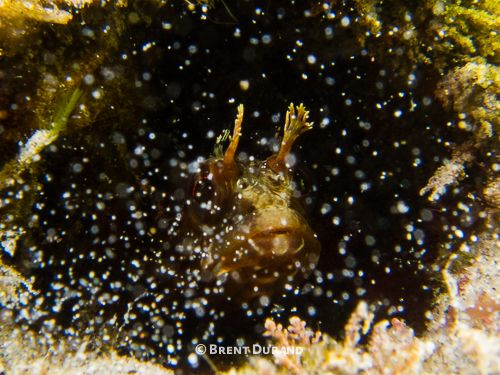
\includegraphics[width=1\linewidth]{assets/backscatter_article_durand2.jpg}
        \caption{}
        % \label{subfig:backscatter_durand}
    \end{subfigure}
    \hfill
    \begin{subfigure}{.49\textwidth}
        \centering
        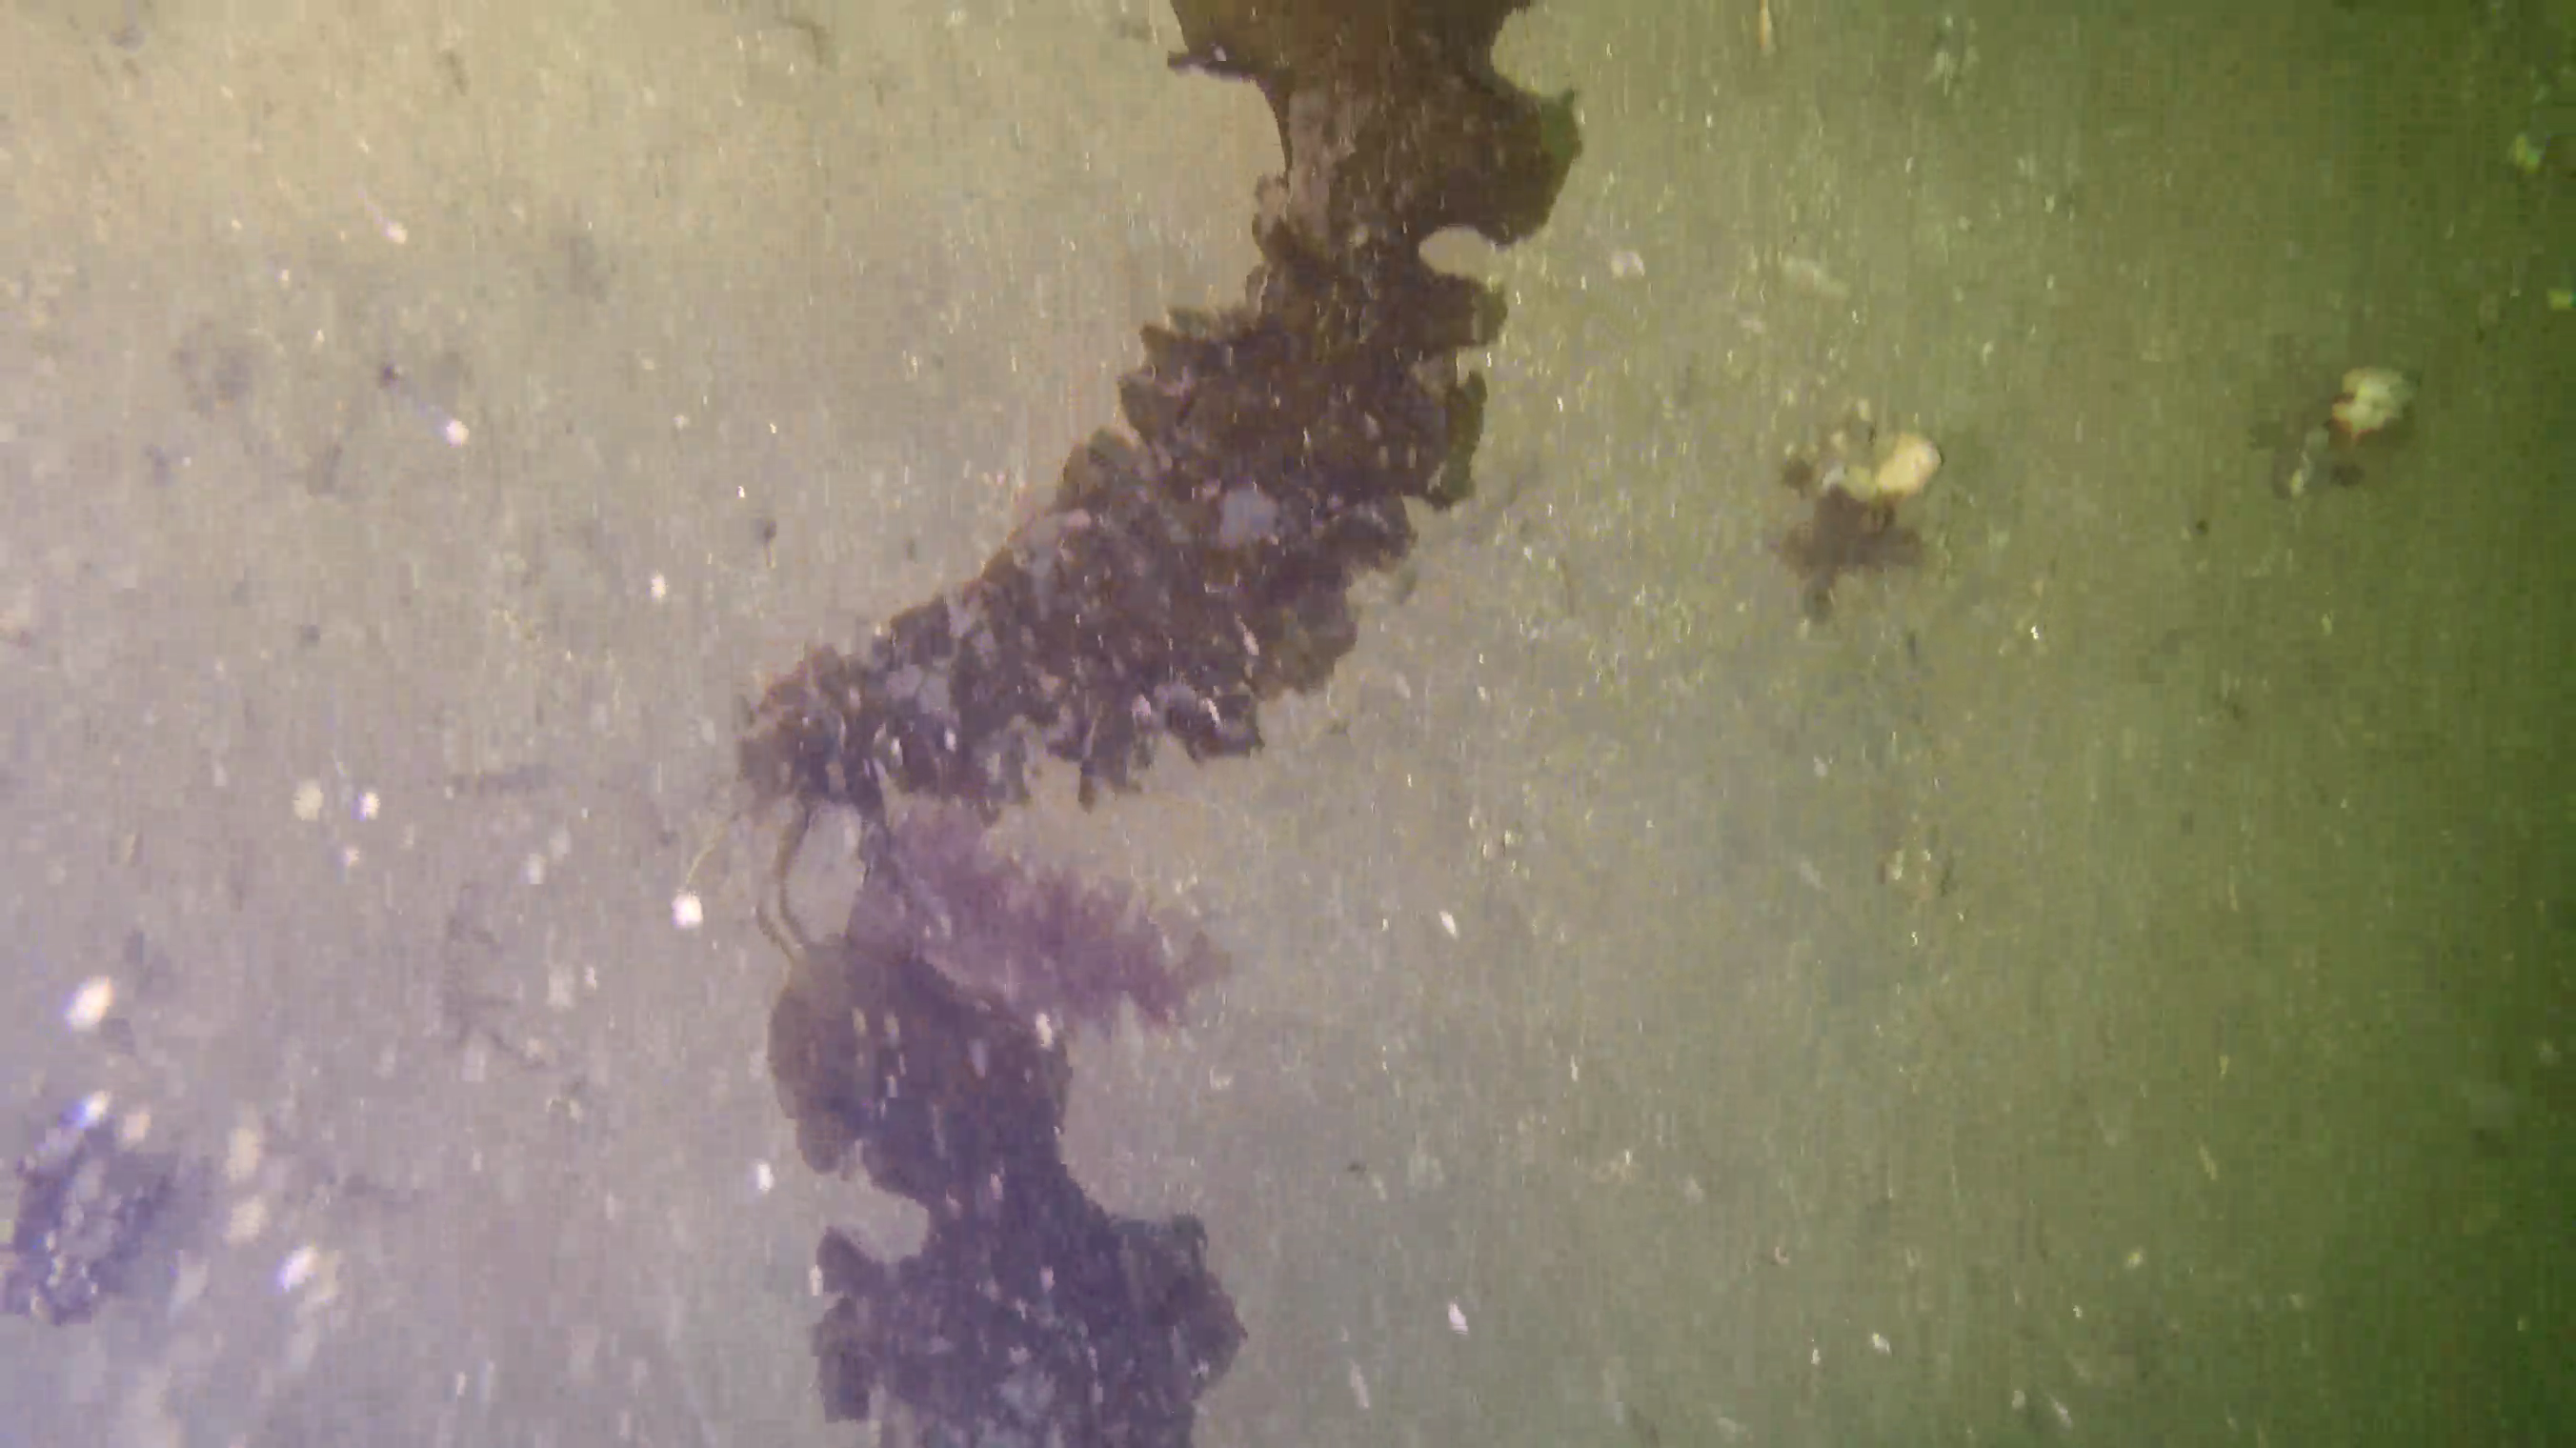
\includegraphics[width=1\linewidth]{assets/backscatter_test_vid.png}
        \caption{}
        % \label{subfig:backscatter_gopro}
    \end{subfigure}
    \caption{(a) Backscatter appears as the particles of sand drift between the aquatic animal and the camera, retrieved from \cite{brentdurandEasyWaysEliminate2013}. (b) A captured frame in GoPro footage from a UUV of the seabed with backscatter increasing as the propellors disrupt the sand.}
    \label{fig:backscatter}
\end{figure}

With a specialised camera sensor to capture fast-moving backscatter particles, a single-board computer processing frames using advanced machine vision technologies to detect backscatter, and a specialised projector to project selectively illuminated light patterns, the project's ultimate goal is to develop a novel backscatter-cancelling light source to aid the generation of high-quality underwater images in real-time, thus eliminating the requirement for a camera with better dynamic range compatibility to compensate for the bright regions from backscatter and lens flares. The first objective is to research architectures to develop a reliable backscatter detection system, tieing in with the second objective of researching methodologies to optimise for real-time to ensure predictability and stability, ensuring the projection of backscatter-cancelling light patterns with minimal and consistent latency.

Section \ref{background} summarises the information in related theoretical realms to form the foundation of the subsequent sections. Section \ref{design} first introduces the assumptions and requirements before detailing the high-level processes for both the lighting system and toolsets for testing. Section \ref{implementation} showcases the system and toolset implementations, which Section \ref{testing} then quantifies by evaluating the real-time performances. Section \ref{conclusion} reflects on these evaluations, including a reflection on project execution and a discussion of future work.


\section{Background Information}
\label{background}
An accurate and real-time backscatter-cancelling lighting system must consider five main factors: (a) precise backscatter particle segmentation even in varying environmental conditions by mapping the exact backscatter positions to aid in (b), the accurate projection of the backscatter cancelling light patterns, ensuring the whole scene except backscatter is lit, (c) low system latency by minimising the time it takes between frame capture and the light pattern projection, ensuring the projection is still correct even with fast-moving backscatter, interlinked with (d), adequate system throughput with parallel processing to increase system responsiveness for reaching the low latency goal, and finally, (e) the ability to control and establish the system frame rate to ensure system predictability.

This section, gathers background information on the five system factors, beginning with an investigation of previous work on this project. Then exploring work related to underwater imaging for precise environmental analysis. Finally, a study on computer systems and architectures for this project and a summary of all aspects concludes the section.

\subsection{Previous Work in Underwater Anti-Backscatter Lighting Systems}
\label{prevwork}

Previous work on this project in \cite{katieshepherdMachineVisionBased2023} by Shepherd introduces a backscatter-cancelling lighting system with goals similar to what this paper proposes. Shepherd presents a two-stage process, which is fundamental to their system, illustrated in Figure \ref{fig:shepherd_system_stages}. The first stage is `detection', where the specialised projector illuminates the whole scene with a low-brightness, solid white output intending to forcefully induce backscatter particles for detection with machine vision techniques. The second stage is `pattern projection', where the system overlays black ellipses called `holes' at the positions of detected backscatter particles over a full-brightness, solid white projection to eliminate backscatter.

\begin{figure}[H]
    \centering
    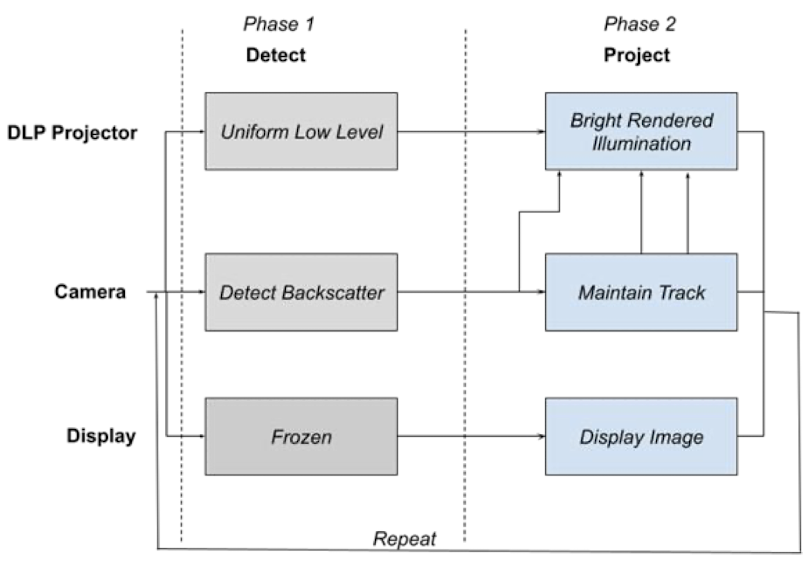
\includegraphics[width=0.7\textwidth]{assets/shepherd_fig6_system.png}
    \caption{The high-level system stages from \cite{katieshepherdMachineVisionBased2023}.}
    \label{fig:shepherd_system_stages}
\end{figure}

Shepherd designs the backscatter segmentation system based on a simple blob detection algorithm \cite{opencvOpenCVCvSimpleBlobDetector}, where the term `blob' denotes a group of connected pixels in a binary image. By applying several thresholds, the algorithm first converts the input image into a binary representation to then extract connected pixels and calculate the centre positions of each. After grouping the centre positions from the binary images, the algorithm finally estimates the final centroid and radii for each `blob'. While this blob detection algorithm benefits from a computationally simple approach, it suffers from a drastic drawback as Shepherd describes ``at least one property needs to be shared between the blobs such as size or shape to allow for the isolation of these blobs''. The underwater environment is unpredictable, where backscatter particles can never share the same characteristics, making this approach unviable.

\subsection{Automotive Headlights for Illumination Through Rain and Snow}
\label{autolights}

Similar to the underwater backscatter that this paper explores and attempts to eliminate, the work in \cite{decharetteFastReactiveControl2012} by De Charette et al. outlines an automotive headlight system to illuminate around the backscatter caused by rain and snow whilst driving. The parallax issue observed by Shepherd, where the displacement between the camera's and projector's viewpoint causes a perceived offset in object positioning, is resolved in De Charette et al. using a beamsplitter arrangement, illustrated in Figure \ref{fig:beamsplitter_system}, such that the incident visual beam is split 50:50 between the projector and camera, thus eliminating parallax displacement by co-location.

\begin{figure}[H]
    \centering
    \begin{subfigure}{.49\textwidth}
        \centering
        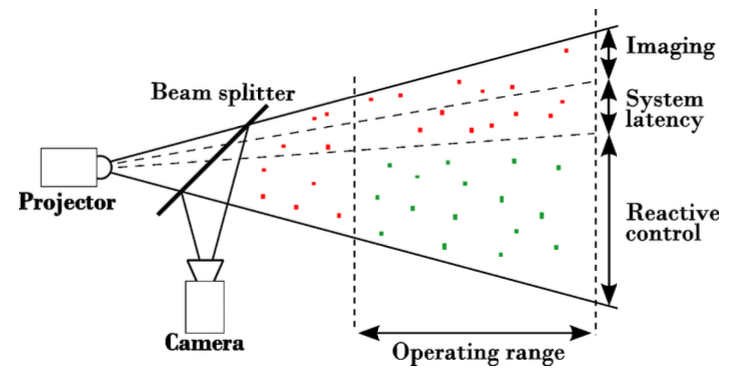
\includegraphics[width=1\textwidth]{assets/beamsplitter_automotive_system.png}
        \caption{}
        \label{fig:beamsplitter_system}
    \end{subfigure}
    \hfill
    \begin{subfigure}{.49\textwidth}
        \centering
        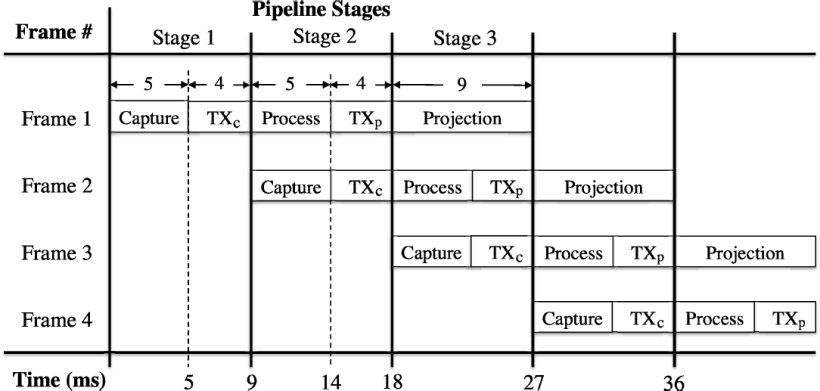
\includegraphics[width=1\textwidth]{assets/cmu_auto_pipeline.png}
        \caption{}
        \label{fig:cmu_auto_pipeline}
    \end{subfigure}
    \caption{From \cite{decharetteFastReactiveControl2012}: (\ref{sub@fig:beamsplitter_system}) The system configuration including a beamsplitter for parallax elimination through co-location, (\ref{sub@fig:cmu_auto_pipeline}) the parallel pipeline stages for their system.}
    \label{fig:decharette}
\end{figure}

The automotive backscatter-cancelling headlight system utilises an image processing pipeline that applies a background subtraction, albeit not specifying the exact method, followed by blurring and thresholding to isolate the bright water spots. The system employs the connected-components algorithm to segment the backscatter particles, this algorithm scans an image to group its pixels into components based on pixel connectivity, i.e., all pixels in a connected component share similar pixel intensity values and are in some way connected \cite{robertfisherConnectedComponentsLabeling2003}. Unlike Shepherd's system which employs a blob detection algorithm, this system is resilient to unique backscatter particle characteristics, allowing for segmentation regardless of fixed parameters despite also being a computationally simple approach. However, the connected-components algorithm may be inherently limited when given low-quality input images as it may not correctly connect pixels due to distortion and noise.

Although not specifying the exact methods, the automotive system in De Charette et al. employs backscatter particle tracking with a predictive algorithm to project backscatter-cancelling light patterns by accounting for the movement during the system processing period, denoted by the system latency time. Due to the linear and vertical movement of rain and snowfall, one can assume they are using a simple linear interpolative approach with the assumption the particles are moving at a constant speed, to predict the future particle position. To increase system throughput, the work in De Charette et al. proposes a three-stage parallel processing pipeline, illustrated in Figure \ref{fig:cmu_auto_pipeline}. Stage 1 represents the task of capturing the frame from the camera, with $TX_c$ denoting the image data transfer from the camera to the computer. Stage 2 represents the image processing steps, with drop detection, prediction, and projection pattern generation, with $TX_p$ denoting the computer-to-projector data transfer. The third and final stage represents the refresh time of the projector. This system, once primed, will run with a three-frame latency: as the $n^{th}$ frame is being captured, the $n^{th} - 1$ frame is being processed, and the $n^{th} - 2$ frame is being projected. With this fixed latency mitigated by the predictive functionality.

The system in De Charette et al. takes, on average across 5500 frames, \SI{4.214}{\milli\second} to transfer data from the camera to the host computer, a \SI{3.2}{\giga\hertz} Intel Xeon processor with \SI{8}{\giga\byte} of RAM running Windows Vista 64-bit, \SI{4.081}{\milli\second} to process the image, \SI{4.214}{\milli\second} to send the data to the projector, and \SI{9}{\milli\second} for the projector to output. Thus, total system latency is \SI{21.51}{\milli\second}, with an accuracy of 68.9\% for rain. The work in \cite{tamburoProgrammableAutomotiveHeadlights2014} by Tamburo et al. expands on the system by De Charette et al. with a more powerful desktop PC for image processing and an FPGA-based controller for the specialised projector. This system achieves an average frame processing time of \SI{0.3}{\milli\second}, with a total response time ranging between \SI{1}{\milli\second} to \SI{2.5}{\milli\second}.

\subsection{Underwater Gas Seepage Bubble Quantification for Environmental Analysis}
\label{gasquant}

Aside from the work by Shepherd, De Charette et al., and Tamburo et al., public documentation of research related to real-time efforts for underwater backscatter-cancelling lighting systems is non-existent. However, numerous environmental analysis fields rely on highly specialised and precise systems for quantifying underwater bubbles to investigate gas seepages from the sea floor. As underwater backscatter can comprise a mixture of compositions, ranging from bubbles and sand to all sorts of marine debris, it will be beneficial to explore gas escape measurement and monitoring systems as they require high precision, extensive range, strong anti-interference, and low cost under complex underwater conditions \cite{zhangUnderwaterBubbleEscape2023}.

The work in \cite{thomanekAutomatedGasBubble2010} by Thomanek et al. presents a novel approach for a highly precise automated gas bubble imaging system that employs the Canny edge detection algorithm. The Canny algorithm, which prefers a single channel (greyscale) input, first smoothens the input using Gaussian convolution before comparing each pixel's values relative to its neighbours such that when the gradient is above a certain threshold, it sets the bordering pixel a value of `1', otherwise `0', resulting in the formation of edges around objects \cite{cannyComputationalApproachEdge1986a}. In contrast to the system by Shepherd, the Canny approach in Thomanek et al. works around the object characteristics limitation of the simple blob detection algorithm.

The paper compares the Canny algorithm approach with the simple image binary thresholding method, where only the pixels with intensities within a certain threshold are passed through, ultimately establishing Canny as the more accurate choice for segmentation, even in areas of uneven illumination, illustrated in Figure \ref{fig:canny_segmentation_compare}. However, the drawbacks of the Canny approach, as highlighted by Thomanek et al., include a significant increase in computing time, and the necessity for implementing morphological techniques to address bubble transformation issues such as expansion and contraction during segmentation. Nevertheless, considering the advancements in computing power over the past 14 years since this paper was published, modern computers should now be easily capable of handling this workload with relative ease.

\begin{figure}[H]
    \centering
    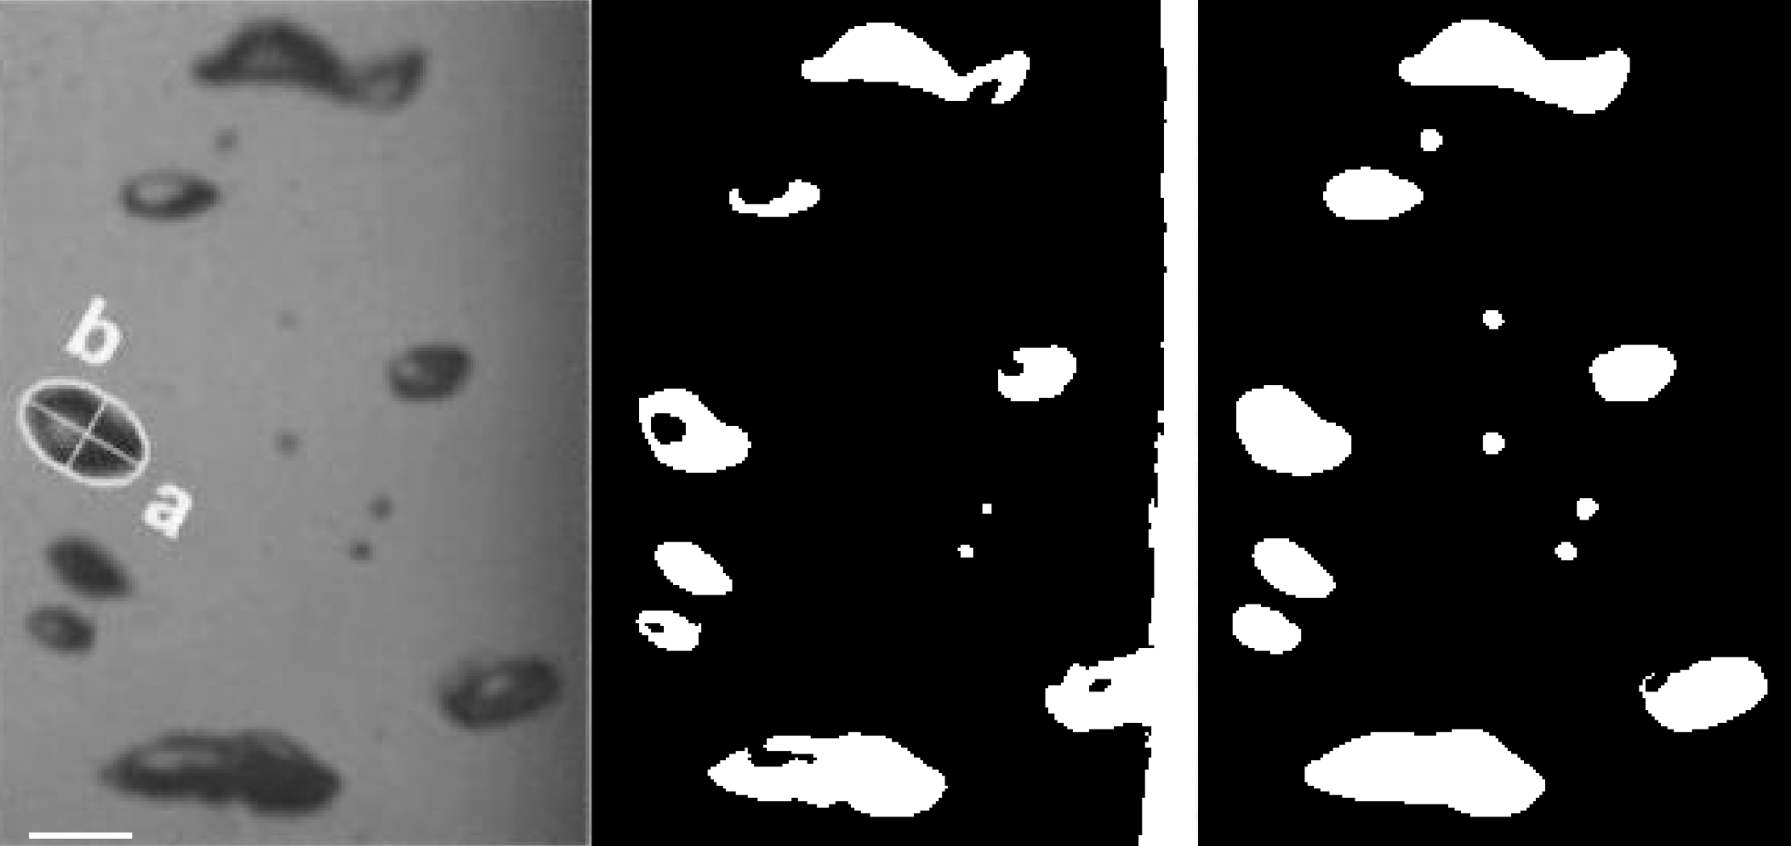
\includegraphics[width=0.7\textwidth]{assets/bubble-segmentation-canny-thresholding.png}
    \caption{From \cite{thomanekAutomatedGasBubble2010}, the original input frame in the left-most image, bubble segmentation using simple binary thresholding in the middle, and bubble segmentation using the Canny edge detection algorithm in the right-most image.}
    \label{fig:canny_segmentation_compare}
\end{figure}

While this paper by Thomanek et al. provides valuable insight and serves as an excellent starting point, it primarily emphasises system construction and quantifying gas flux measurements. Consequently, certain crucial details, such as the precise methodology employed for achieving the highlighted bubbles post-Canny segmentation in Figure \ref{fig:canny_segmentation_compare}, receive less attention. However, one can infer that Thomanek et al. may have employed a logical algorithm to fill closed-loop edges. The study by Zelenka in \cite{zelenkaGasBubbleShape2014a} builds upon the foundational system by Thomanek et al. aiming to address the sporadic false detection issue that is inherent in the Canny edge detection algorithm, introducing robust algorithms capable of achieving precise bubble stream quantification with accurate bubble fitting.

Zelenka introduces a snake-based active contour model developed by Kass et al. in \cite{kassSnakesActiveContour1988} for a more stable and precise method for bubble detection. As explained by Kass et al., a snake embodies an energy-minimising spline that's guided by external forces and influenced by image characteristics that collectively drive the snake towards prominent features within the image, such as lines and edges, all while the snake dynamically adheres to nearby edges due to the active contour model. The classic snake method, illustrated in Figure \ref{subfig:classic_snake}, uses a bounding box from the baseline localisation for initialisation, shown in blue, from which the snake algorithm optimises with each iteration on a low-quality image sequence. The figure exemplifies the unreliability of the classic snake method due to light areas within the centre of the bubble, as the red outline borders this region instead of the bubble itself. Zelenka, therefore, introduces a novel enhancement to the classic snake method to improve performance in varying lighting conditions by utilising gradient information of an image to compute external energy terms that guide the snake.

Zelenka compares all of these bubble segmentation methods using a sequence of 20 GoPro-captured images, with circa 10 bubbles visible per frame and manual ground truth. The results, illustrated in Figure \ref{fig:zelenka_performance}, show a clear improvement across all methods compared to the baseline Canny approach, which achieved a detection rate of 77.3\%. The classic snake approach achieved the best detection rate of 89.7\% and the gradient-snake achieved 89.3\%.

\begin{figure}[H]
    \centering
    \begin{subfigure}{.49\textwidth}
        \centering
        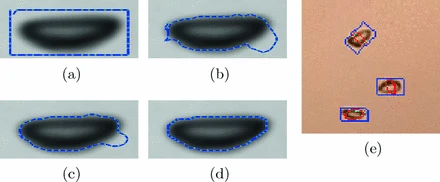
\includegraphics[width=1\linewidth]{assets/classic_snake.png}
        \caption{Classic snake algorithm.}
        \label{subfig:classic_snake}
    \end{subfigure}
    \hfill
    \begin{subfigure}{.49\textwidth}
        \centering
        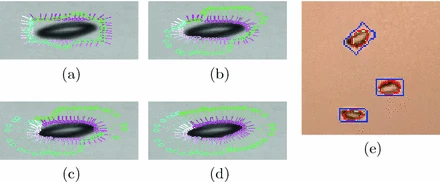
\includegraphics[width=1\linewidth]{assets/gradient_snake.png}
        \caption{Gradient-based snake algorithm.}
        \label{subfig:gradient_snake}
    \end{subfigure}
    \caption{The classic snake method in (\ref{sub@subfig:classic_snake}) and the gradient snake method in (\ref{sub@subfig:classic_snake}) from \cite{zelenkaGasBubbleShape2014a}. Sub-subfigures from (a) to (d) for both methods show every third step in the snake optimisation process, and (e) shows the final result.}
    \label{fig:snake_methods}
\end{figure}

\begin{figure}[H]
    \centering
    \begin{subfigure}{.40\textwidth}
        \centering
        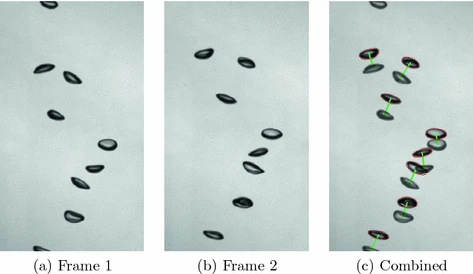
\includegraphics[width=1\textwidth]{assets/zelenka_system.png}
        \caption{}
        \label{fig:zelenka_system}
    \end{subfigure}
    \hfill
    \begin{subfigure}{.55\textwidth}
        \centering
        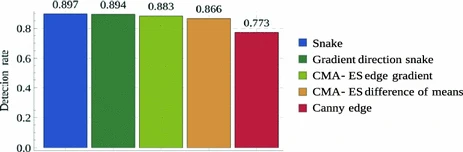
\includegraphics[width=1\textwidth]{assets/zelenka_performance.png}
        \caption{}
        \label{fig:zelenka_performance}
    \end{subfigure}
    \caption{From \cite{zelenkaGasBubbleShape2014a}: (\ref{sub@fig:zelenka_system}) demonstration of the system across two subsequent frames at 100 FPS, with the red border denoting bubble detection and the green lines denoting bubble tracking, (\ref{sub@fig:zelenka_performance}) a comparison of bubble detection rates for different segmentation approaches.}
    \label{fig:zelenka}
\end{figure}

Thomanek et al. introduced a novel approach for bubble tracking, leveraging the `least distance assumption'. This assumption entails realising that the distance travelled by a bubble between two successive frames is typically smaller than the distance to its closest neighbouring bubble. While this assumption may not hold for scenarios involving overlapping bubbles, extremely high bubble concentrations, or cases where the travel distance exceeds the distances to neighbouring bubbles, it, however, facilitates a computationally straightforward method for determining bubble positions in successive frames and estimating the bubble rise velocity from the sea floor. Despite the computation simplicity, this method may not present a fair trade-off due to the backscatter originating from bubbles, which can be highly concentrated, overlapping, and subject to rapid movement, especially in the presence of UUV propellers. Zelenka's paper introduces a novel approach for tracking bubbles by employing a Kalman filter \cite{kalmanNewApproachLinear1960} to predict bubble positions in subsequent frames based on initial detections. The Kalman filter utilises a recursive algorithm to estimate the state of a dynamic system, in this case, the bubble's position, by incorporating both prediction and measurement update steps. Additionally utilising, the Hungarian method \cite{kuhnHungarianMethodAssignment1955}, which finds the optimal assignment in a weighted graph, for minimum weighted matching between predicted and newly detected bubble positions, optimising the association process. While it remains uncertain whether the Kalman filter-based method is immune to the limitations associated with the `least distance assumption', Zelenka does validate its capacity as a highly reliable tracking mechanism. An illustration of the whole system from Zelenka is illustrated in Figure \ref{fig:zelenka_system}, showing both bubble detection and tracking.

\subsection{System Building Blocks}
\label{buildingblocks}

\subsubsection{Real-Time Linux Kernel with the PREEMPT-RT Patch}
\label{preempt}

Shepherd's work highlighted the necessity of employing a Real-Time Operating System (RTOS) to mitigate jittering, the unpredictable bursts of reduced frame rates. An RTOS facilitates the compliance of a `hard' real-time system, which can provide a guarantee of the maximum time a task necessitates for completion. Similar to Shepherd's system, in Linux, many sections in kernel space, where the kernel's code and data reside and execute, do not support preemption due to the presence of spinlocks. Spinlocks are non-blockable and non-sleepable programmatic loops that safeguard critical sections of code. Consequently, the preemption logic breaks down when a user space task invokes a kernel-specific function, thereby transitioning to kernel space upon receiving an interrupt. 

Figure \ref{fig:bootlin_flow}, depicted in the material from \cite{bootlinUnderstandingLinuxRealtime2024} by Bootlin, highlights how kernel-based spinlocks contribute to unpredictable jitter, as denoted by the green question mark. Apart from the kernel space incompatibility, Linux already facilitates user space preemption through task priority-based real-time scheduling, enabling RTOS functionality. The PREEMPT-RT kernel patch modifies all kernel-space code, allowing it to become preemptible and deterministic. While insufficient in transforming Linux into a `hard' RTOS, the PREEMPT-RT patch minimises task-switching latencies. Using a test suite that contains programs to test various real-time Linux parameters, the material in \cite{maurorivaRaspberryPi4B2019} compares system latencies with the PREEMPT-RT patch. The results are in Figure \ref{fig:lemariva_latency}, displaying the maximum latency measurements obtained with the standard kernel, registering at \SI{301}{\micro\second}, whereas the PREEMPT-RT kernel yielded a significantly reduced latency of \SI{83}{\micro\second}, a notable 3.63x reduction.

\begin{figure}[H]
    \centering
    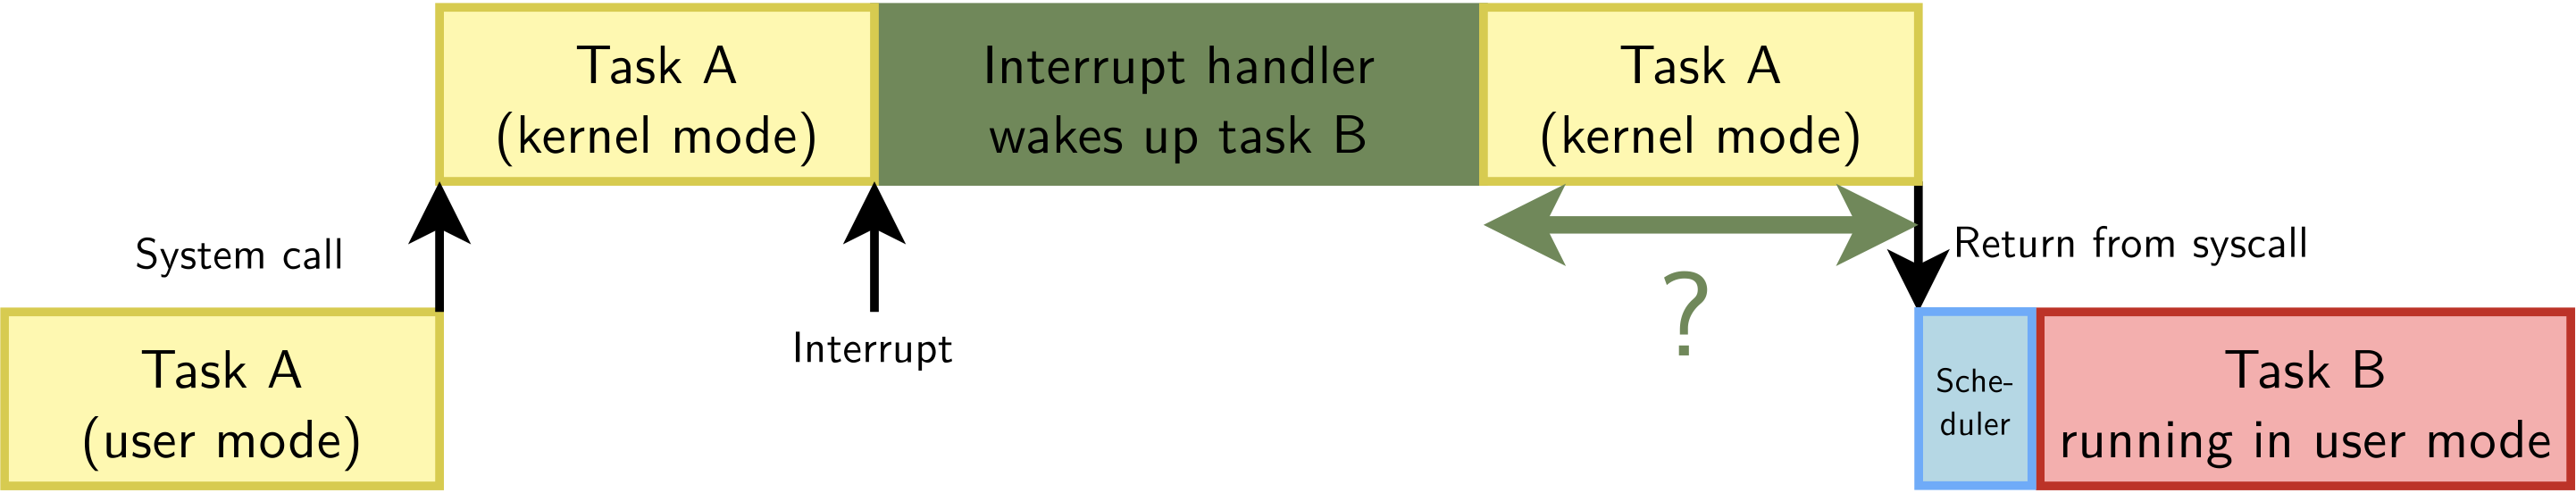
\includegraphics[width=1\textwidth]{assets/bootlin-interrupt-flow.png}
    \caption{From \cite{bootlinUnderstandingLinuxRealtime2024}, illustrating kernel-space latency from an interrupt in the Linux kernel.}
    \label{fig:bootlin_flow}
\end{figure}

\begin{figure}[H]
    \centering
    \begin{subfigure}{.49\textwidth}
        \centering
        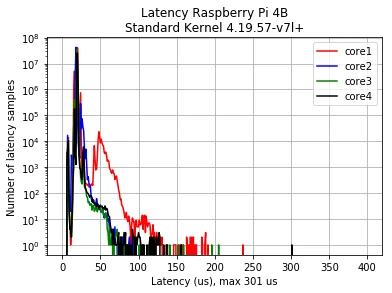
\includegraphics[width=1\linewidth]{assets/lemariva-std-kernel-latency.png}
        \caption{}
        \label{fig:std_latency}
    \end{subfigure}
    \hfill
    \begin{subfigure}{.49\textwidth}
        \centering
        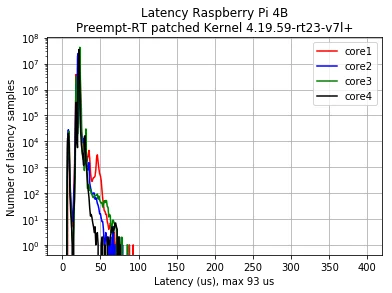
\includegraphics[width=1\linewidth]{assets/lemariva-rt-kernel-latency.png}
        \caption{}
        \label{fig:rt_latency}
    \end{subfigure}
    \caption{Latency measurements from \cite{maurorivaRaspberryPi4B2019} using Cyclictest from the RT-Tests suite. (\ref{sub@fig:std_latency}) The standard Linux RPi kernel, and (\ref{sub@fig:rt_latency}) the PREEMPT-RT kernel.}
    \label{fig:lemariva_latency}
\end{figure}

\subsubsection{Computing Platforms}
Field Programmable Gate Arrays (FPGAs), semiconductor devices structured around a matrix of configurable logic blocks (CLBs) interconnected via programmable interconnects \cite{WhatFPGAField}, are ideal solutions for computationally demanding image processing tasks, owing to their inherent hardware parallelism and low latency characteristics. Despite the availability of highly efficient intellectual property (IP) cores for FPGA-based logic acceleration, development and prototyping times may increase due to the intricate low-level hardware intricacies involved. Additionally, FPGAs typically incur higher costs compared to traditional CPU-based computing systems. On the other hand, the Raspberry Pi (RPi) company has been at the forefront of designing high-performance, cost-effective, single-board, and modular computers based on the Arm architecture and running the Linux operating system since 2012 \cite{raspberrypiltdRaspberryPiUs}. The standard RPi product lineup provides an excellent non-FPGA, CPU-based route for swift and straightforward development and deployment.

\subsubsection{Specialised Light Source}

A Digital Light Processing (DLP) projector plays a crucial role in projecting backscatter-cancelling light patterns. The DLP chipset comprises a Digital Micromirror Device (DMD), which houses millions of reflective aluminium mirrors, typically only a few microns wide. The DMD serves as a Micro-Opto-Electro-Mechanical System (MOEMS) Spatial Light Modulator (SLM), enabling the modulation and attenuation of an incident light beam with precision. As Figure \ref{fig:dmd_dlp} illustrates, a beam emitted from a high-intensity white lamp is directed towards a rotating colour-tinted lens wheel. Subsequently, an internal lens diffracts the coloured beam onto the DMD. The angle and duration of each microscopic mirror's activation dictate the intensity of individual pixels, redirecting the desired beams of each pixel through a diffraction lens to exit the projector. Inactive DMD mirrors direct the beam into a light-absorbing region to prevent light leakage and ensure image integrity.

\begin{figure}[H]
    \centering
    \begin{subfigure}{.4\textwidth}
        \centering
        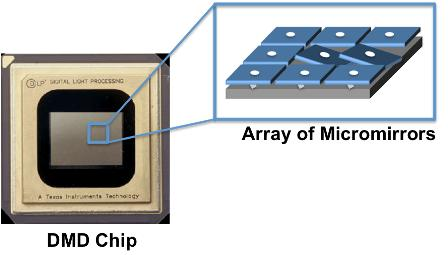
\includegraphics[width=1\linewidth]{assets/dmd-chip.jpg}
        \caption{}
        % \label{subfig:dmd_chip}
    \end{subfigure}
    % \hfill
    \hfill
    \begin{subfigure}{.49\textwidth}
        \centering
        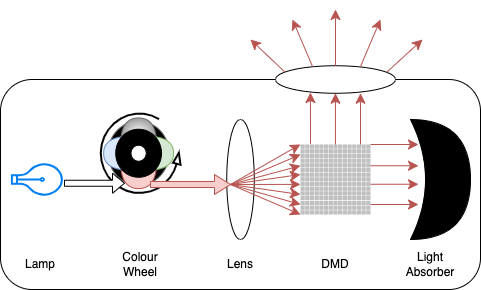
\includegraphics[width=1\linewidth]{assets/dlp-projector.png}
        \caption{}
        % \label{subfig:dlp_projector}
    \end{subfigure}
    \caption{(a) The microscopic mirror array within a DMD chip \cite{HowDoesDLP}. (b) Cross-sectional view of an example projector employing DLP technology.}
    \label{fig:dmd_dlp}
\end{figure}

\subsubsection{Specialised Camera Sensor}

The cameras found in many traditional and consumer-grade electronic devices, including smartphones, typically utilise a CMOS sensor equipped with a rolling shutter. These sensors introduce distortion effects when capturing fast-moving subjects, attributed to their line-by-line scan image-capturing characteristic. A global shutter sensor captures a snapshot of the scene using all pixels simultaneously, rather than line-by-line. Figures \ref{subfig:rs_timeline} and \ref{subfig:gs_timeline} depict the distinctions in image capture between a rolling shutter and a global shutter, and Figure \ref{subfig:rs_vs_gs} showcases capture differences. The Raspberry Pi company offers a global shutter camera with plug-and-play compatibility with Raspberry Pi computers.

\begin{figure}[H]
    \centering
    \begin{subfigure}{.45\textwidth}
        \centering
        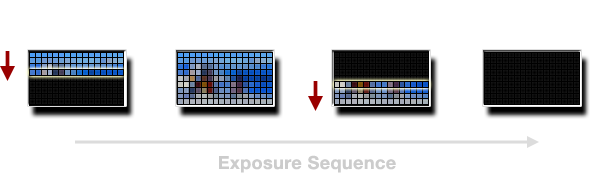
\includegraphics[width=1\linewidth]{assets/rolling-shutter-timeline.png}
        \caption{}
        \label{subfig:rs_timeline}
    \end{subfigure}
    \hfill
    \begin{subfigure}{.45\textwidth}
        \centering
        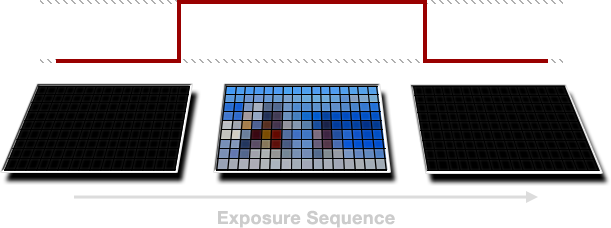
\includegraphics[width=1\linewidth]{assets/global-shutter-timeline.png}
        \caption{}
        \label{subfig:gs_timeline}
    \end{subfigure}
    \hfill
    \begin{subfigure}{0.45\textwidth}
        \centering
        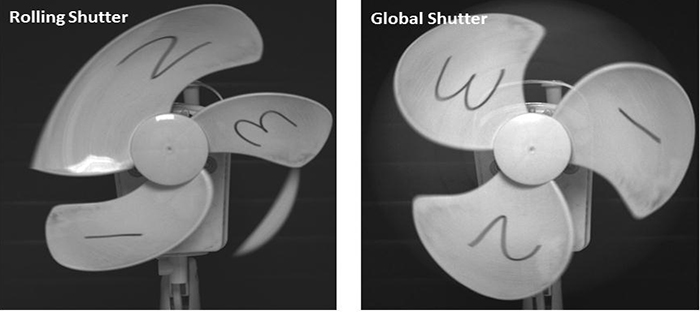
\includegraphics[width=0.7\textwidth]{assets/rolling-vs-global-shutter.jpeg}
        \caption{}
        \label{subfig:rs_vs_gs}
    \end{subfigure}
    \caption{The image capture of a rolling shutter sensor in (\ref{sub@subfig:rs_timeline}) and that of a global shutter in (\ref{sub@subfig:gs_timeline}) \cite{reddigitalcinemaGlobalRollingShutters}, and (\ref{sub@subfig:rs_vs_gs}), the comparison between the sensors when capturing a fast-moving target \cite{RollingShutterVs}.}
    \label{fig:rs_vs_gs}
\end{figure}

\subsection{Summary}
\label{bisummary}

From the background research, the best methodology for precise backscatter segmentation is the Canny edge detection approach due to its resilience in varying particle appearances, a limitation of Shepherd's simple blob detection approach, and robustness in detecting edges even in uneven illumination conditions, exemplified by Thomanek et al. drawing comparisons with simple image thresholding. Zelenka's use of the gradient-based Snake method, despite its capability to segment bubbles with bright spots inside them, is unnecessary for this project's objective, as the focus lies on eliminating just the backscatter within sediments, the bright spot within bubbles, sand, and other marine debris, rather than the entire sediment particle.

When considering the computing platform, a Raspberry Pi single-board computer (SBC) running a Linux OS, and developing the system with Python and OpenCV, an open-source computer vision and machine learning software library with over 2500 optimised algorithms \cite{opencv}, is preferable over an FPGA for its cost-effectiveness, ease of development, and compatibility with a wide range of peripherals and software, aspects which are all essential for this project for prototyping in short time constraints. While a Raspberry Pi SBC that runs an ordinary Linux OS is not inherently a `hard' real-time system like an FPGA implementation, implementing the PREEMPT-RT Linux kernel patch offers improved determinism and reduced latency compared to a standard Linux OS, crucial for ensuring timely and predictable response in the system.

A DLP projector is the preferred choice for projecting backscatter-cancelling light patterns due to its precise control and modulation capabilities, essential for accurately overlaying patterns to eliminate backscatter. Opting for a global shutter camera sensor over a rolling shutter sensor mitigates distortion effects caused by fast-moving subjects, ensuring accurate image capture in dynamic underwater environments.


\section{Design}
\label{design}
This section aims to explore the hardware setup and constraints, outlining key components and requirements for the system and toolsets, and concluding with a summary of the architectures and designs to aid in the subsequent implementation and testing phases.

\subsection{System Equipment \& Design Constraints}
\label{designconstraints}

The system follows from the hardware constraints and assumptions that were set by Shepherd. In this prototype system, as Figure \ref{fig:submersible} illustrates, a plywood plate fastens the custom-fabricated and watertight tubes. The larger of the two tubes houses the Optoma ML550 projector, which features an LED lamp enabling a brightness capability of up to \SI{500}{\lumen}, illuminating a \SI{1}{\centi\metre} DLP for a native resolution of 1280x800, with a maximum \SI{120}{\hertz} vertical and \SI{100}{\kilo\hertz} horizontal scan rate capabilities. The smaller tube houses the RPi 5 (\SI{8}{\giga\byte} RAM variant) SBC, using a Broadcom BCM2712 \SI{2.4}{\giga\hertz} quad-core 64-bit Arm Cortex-A76 CPU to feature an advertised 2-3x performance upgrade from the RPi 4 that Shepherd used.

Connected to this RPi, via a 4-lane Mobile Industry Processor Interface (MIPI) transceiver, is an RPi global shutter (GS) camera, featuring the Sony IMX296LQR-C 1.58MP sensor. Instead of a GS sensor, Shepherd employed the RPi High-Quality (HQ) sensor, however, due to the reasons which Section \ref{designrec} outlines, the GS sensor replaces this. The GS camera uses a PT361060M3MP12 lens, with an adjustable F1.2 aperture, a \SI{6}{\milli\metre} adjustable focal length for a minimum object distance of \SI{0.2}{\metre}, and a field of view of \SI{63}{\degree}. Mounting all components within their respective tubes with 3D-printed mounts, such that the separation between the camera and projector lenses is \SI{12}{\centi\metre}. At the backside of each tube is a metallic cap with watertight cable couplers to pass through the RPi and projector power cables, and an ethernet cable for the RPi.

\begin{figure}[H]
    \centering
    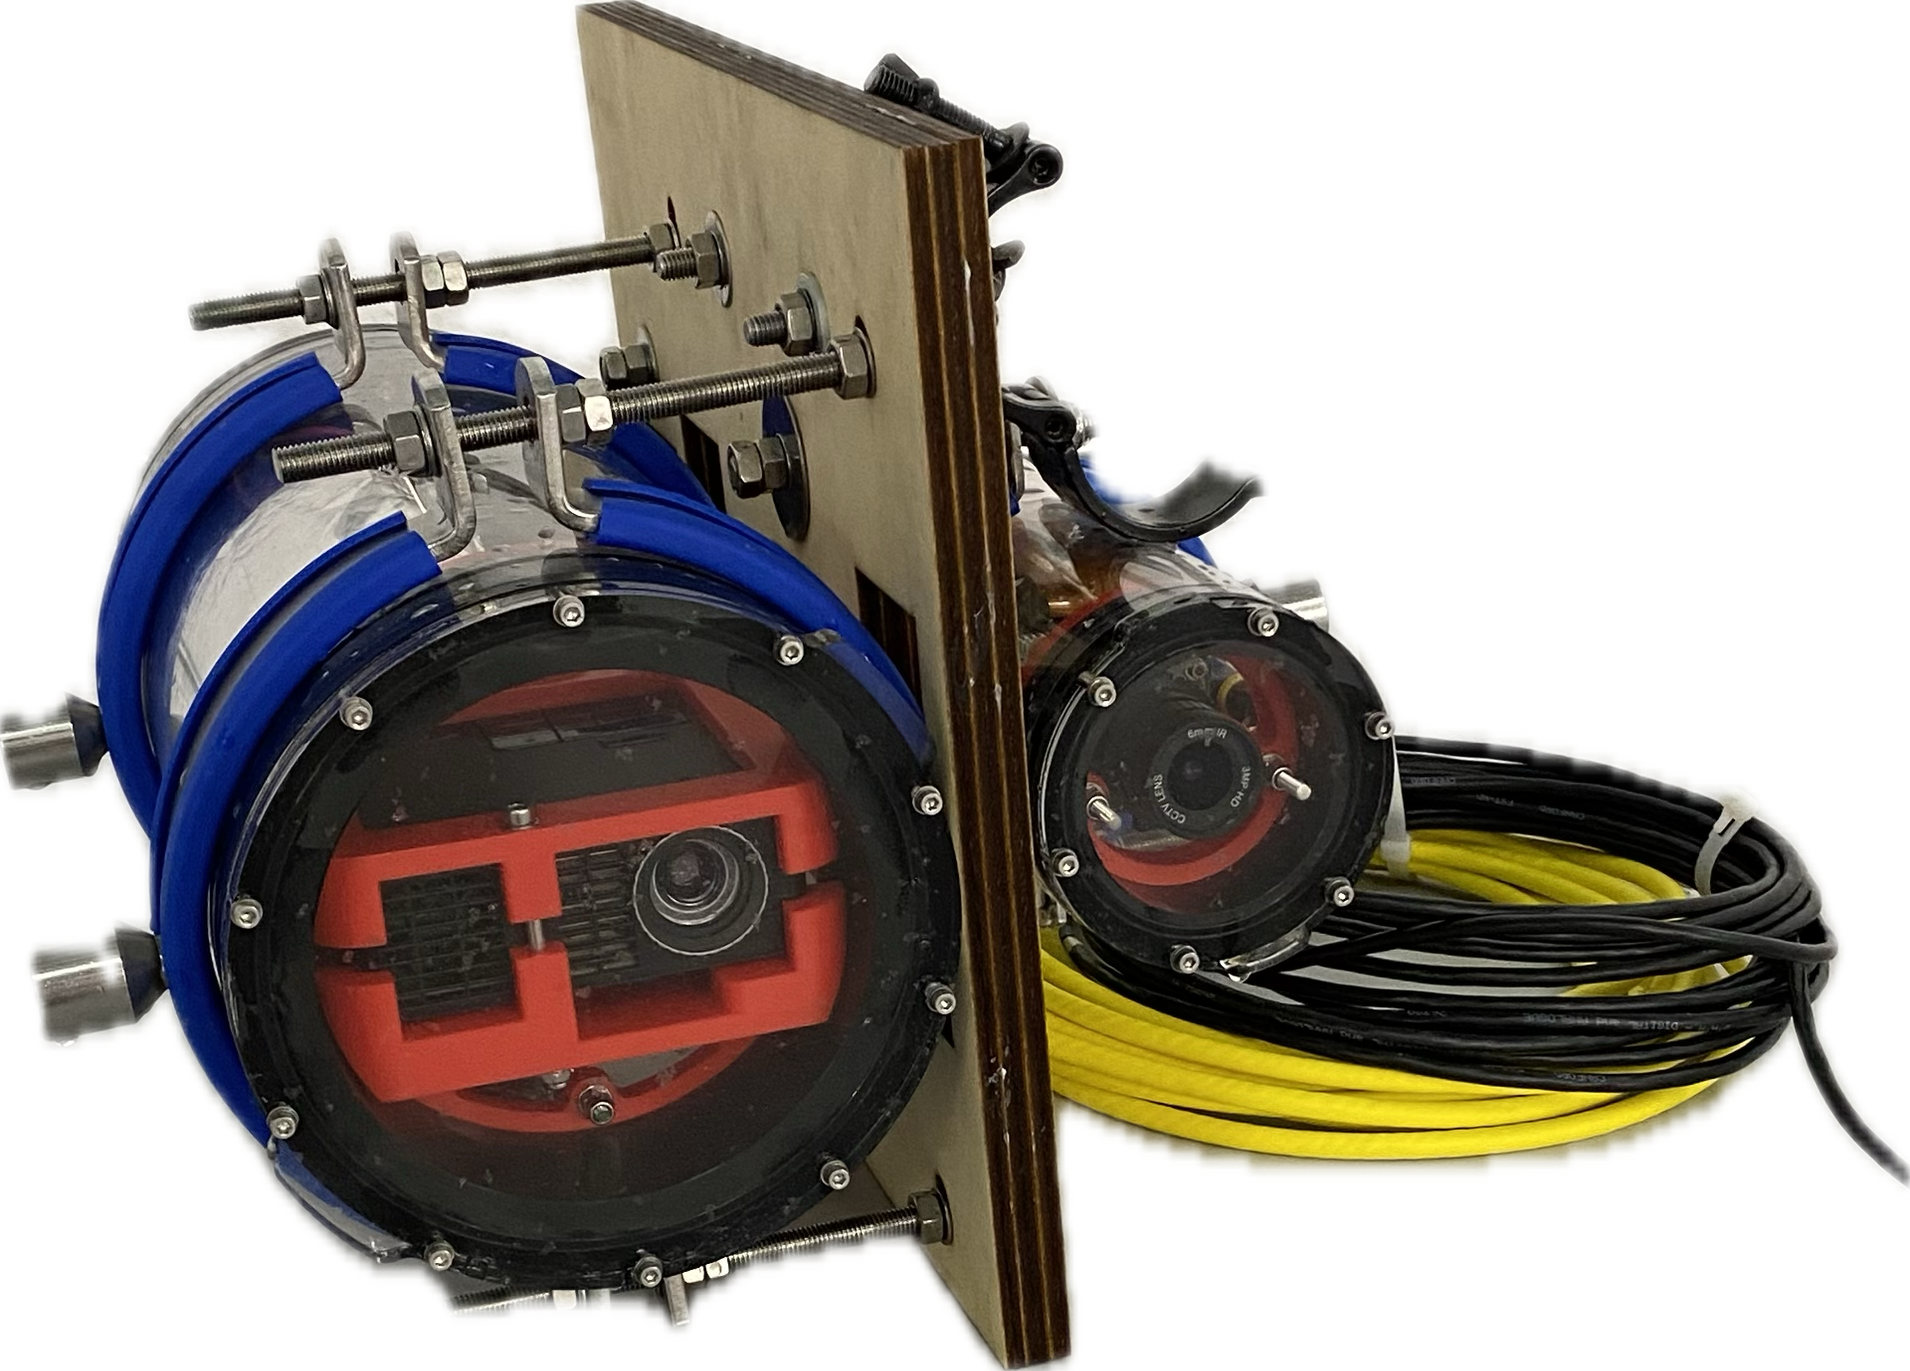
\includegraphics[width=0.8\textwidth]{assets/submersible.png}
    \caption{The submersible system.}
    \label{fig:submersible}
\end{figure}

The design relies on two assumptions: (a) the system is to run below the ocean twilight zone, which is approximately \SI{200}{\metre} below the surface, ensuring the scene is only lit by the system and not other sources such as sunlight, and (b) there are no internal reflections from the housing, such as from the plastic tubes and tube lenses, ensuring all noticeable reflection to be backscatter particles. Due to its watertight construction, disassembling and reassembling the housing is a laborious process, often requiring the reapplication and testing of seals, which can extend the downtime to multiple days. Therefore, this project must prefer conducting tests using pre-recorded footage or synthetic simulations of backscatter to minimise disruptions and maintain operational efficiency.

\subsection{Simulating Backscatter for Synthetic Ground Truth}
\label{designsim}

Given the substantial weight of the submersible, manoeuvring the system into position within an underwater testing tank presents significant challenges during testing. Moreover, the availability of the underwater testing tank at the Institute for Safe Autonomy wasn't fully realised until the later stages of this project. Consequently, there is a need for software capable of synthetically generating a simulation of backscatter particles. Since this simulation is entirely software-based, it must produce ground truth data comprising a dataset, assigning each backscatter particle with a unique ID, allowing for the tracking of coordinates across every frame of the simulation. Comparing the detected backscatter positions from the system with the true positions derived from the simulation ground truth enables the accurate assessment of the system's accuracy and performance.

Employing a straightforward model involving bubbles rising from the bottom of the screen can form a sufficient simulation of random backscatter particle movement in all axis directions: horizontal (x), vertical (y), and towards the camera (z). The simulation can depict backscatter particles as a white circle against a black background for simplicity, with user control over these exact colours. The model should also take into account the bubble expansion due to the pressure difference as they ascend from underwater. As a result, a separate model to simulate bubble distance from the camera location may not be necessary. It's also crucial to model horizontal bubble movement to capture the full range of particle motion.

\subsection{Recording Lossless Video for Physical Testing}
\label{designrec}

At the start of this project, Ben provided me with a GoPro recording from a submersible capturing the seabed, intending to use it as test material to develop the system. However, due to the GoPro's heavy video compression, coupled with its rolling shutter sensor, the video contains a large number of compression artefacts and significant motion blur, as Figure \ref{fig:gopro} illustrates. These issues significantly complicate the task of identifying individual backscatter particles for segmentation, with the system in Figure \ref{fig:submersible} originally, in Shepherd's work, employing an RPi HQ sensor, which is also a rolling-shutter sensor. The limitations posed by the GoPro footage proved the necessity for a GS sensor, prompting the exploration and subsequent implementation of the RPi GS camera. In order to capture test footage using this system, there must be a program in place to record the `raw' footage from the camera, directly from the sensor inside the submersible without any lossy compression.

\begin{figure}[H]
    \centering
    \begin{subfigure}{.49\textwidth}
        \centering
        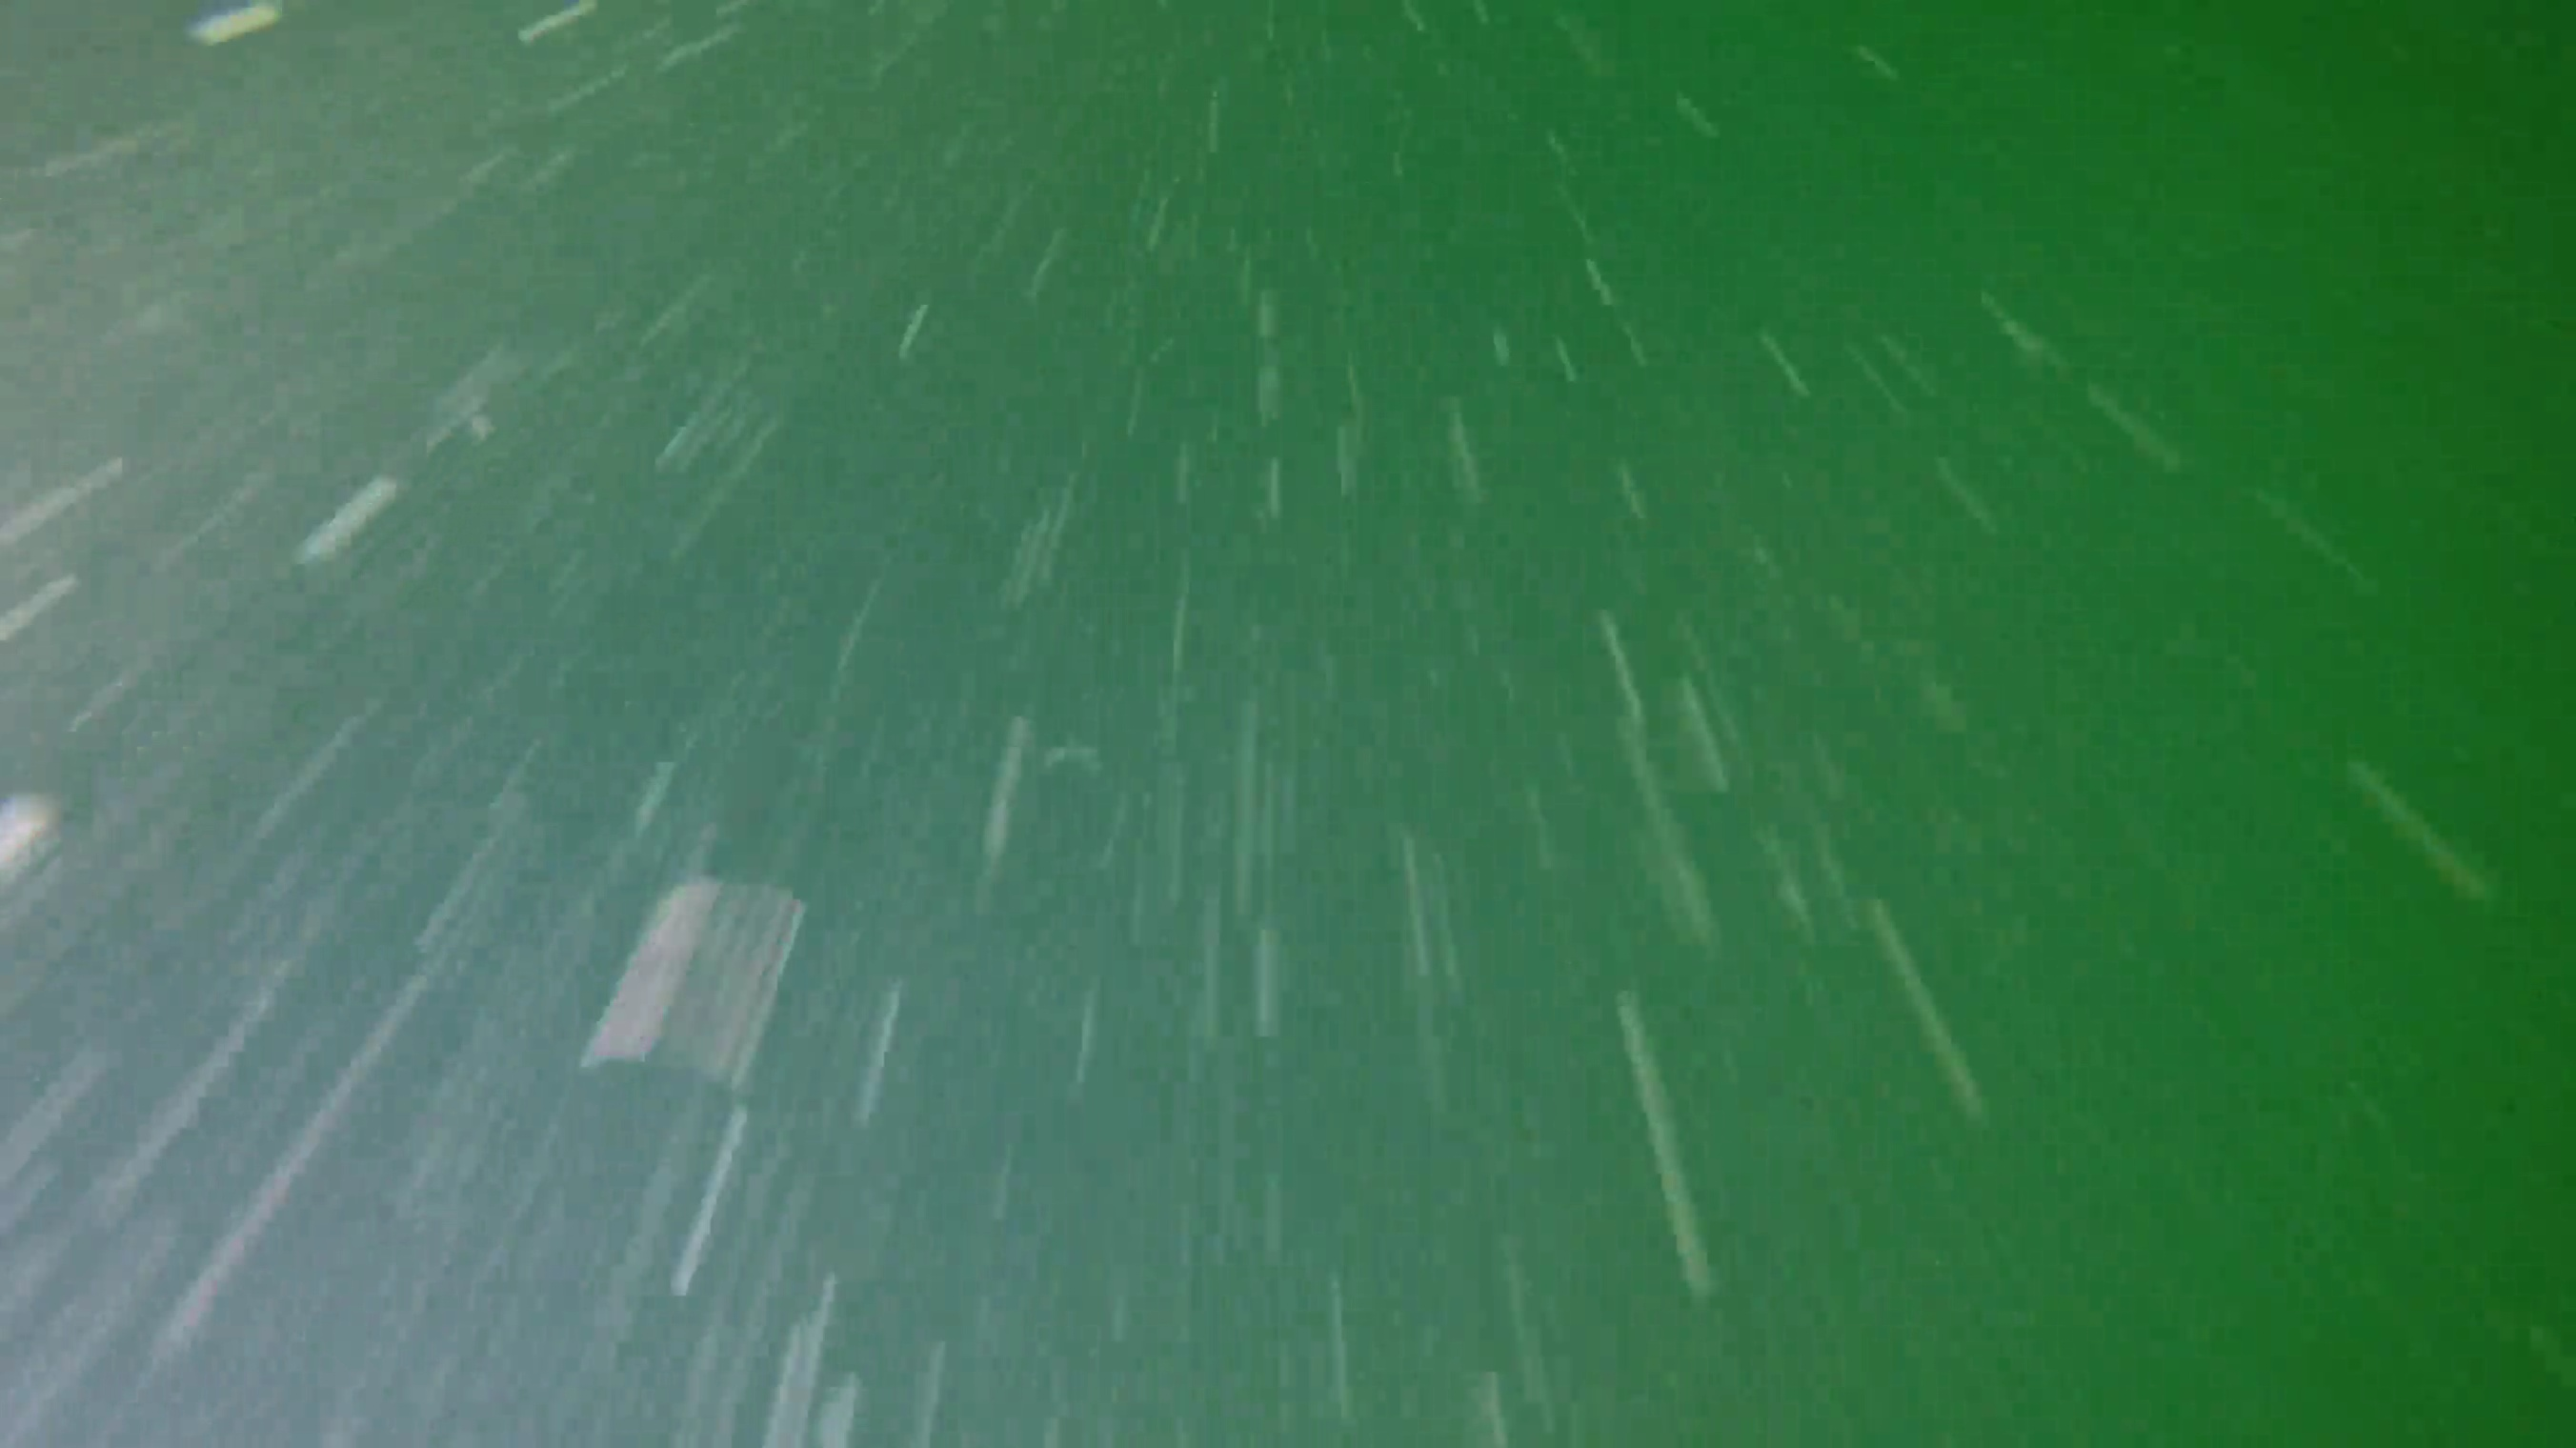
\includegraphics[width=1\linewidth]{assets/gopro_footage_streaks.jpg}
        \caption{}
        \label{fig:motionblur}
    \end{subfigure}
    % \hfill
    \hfill
    \begin{subfigure}{.49\textwidth}
        \centering
        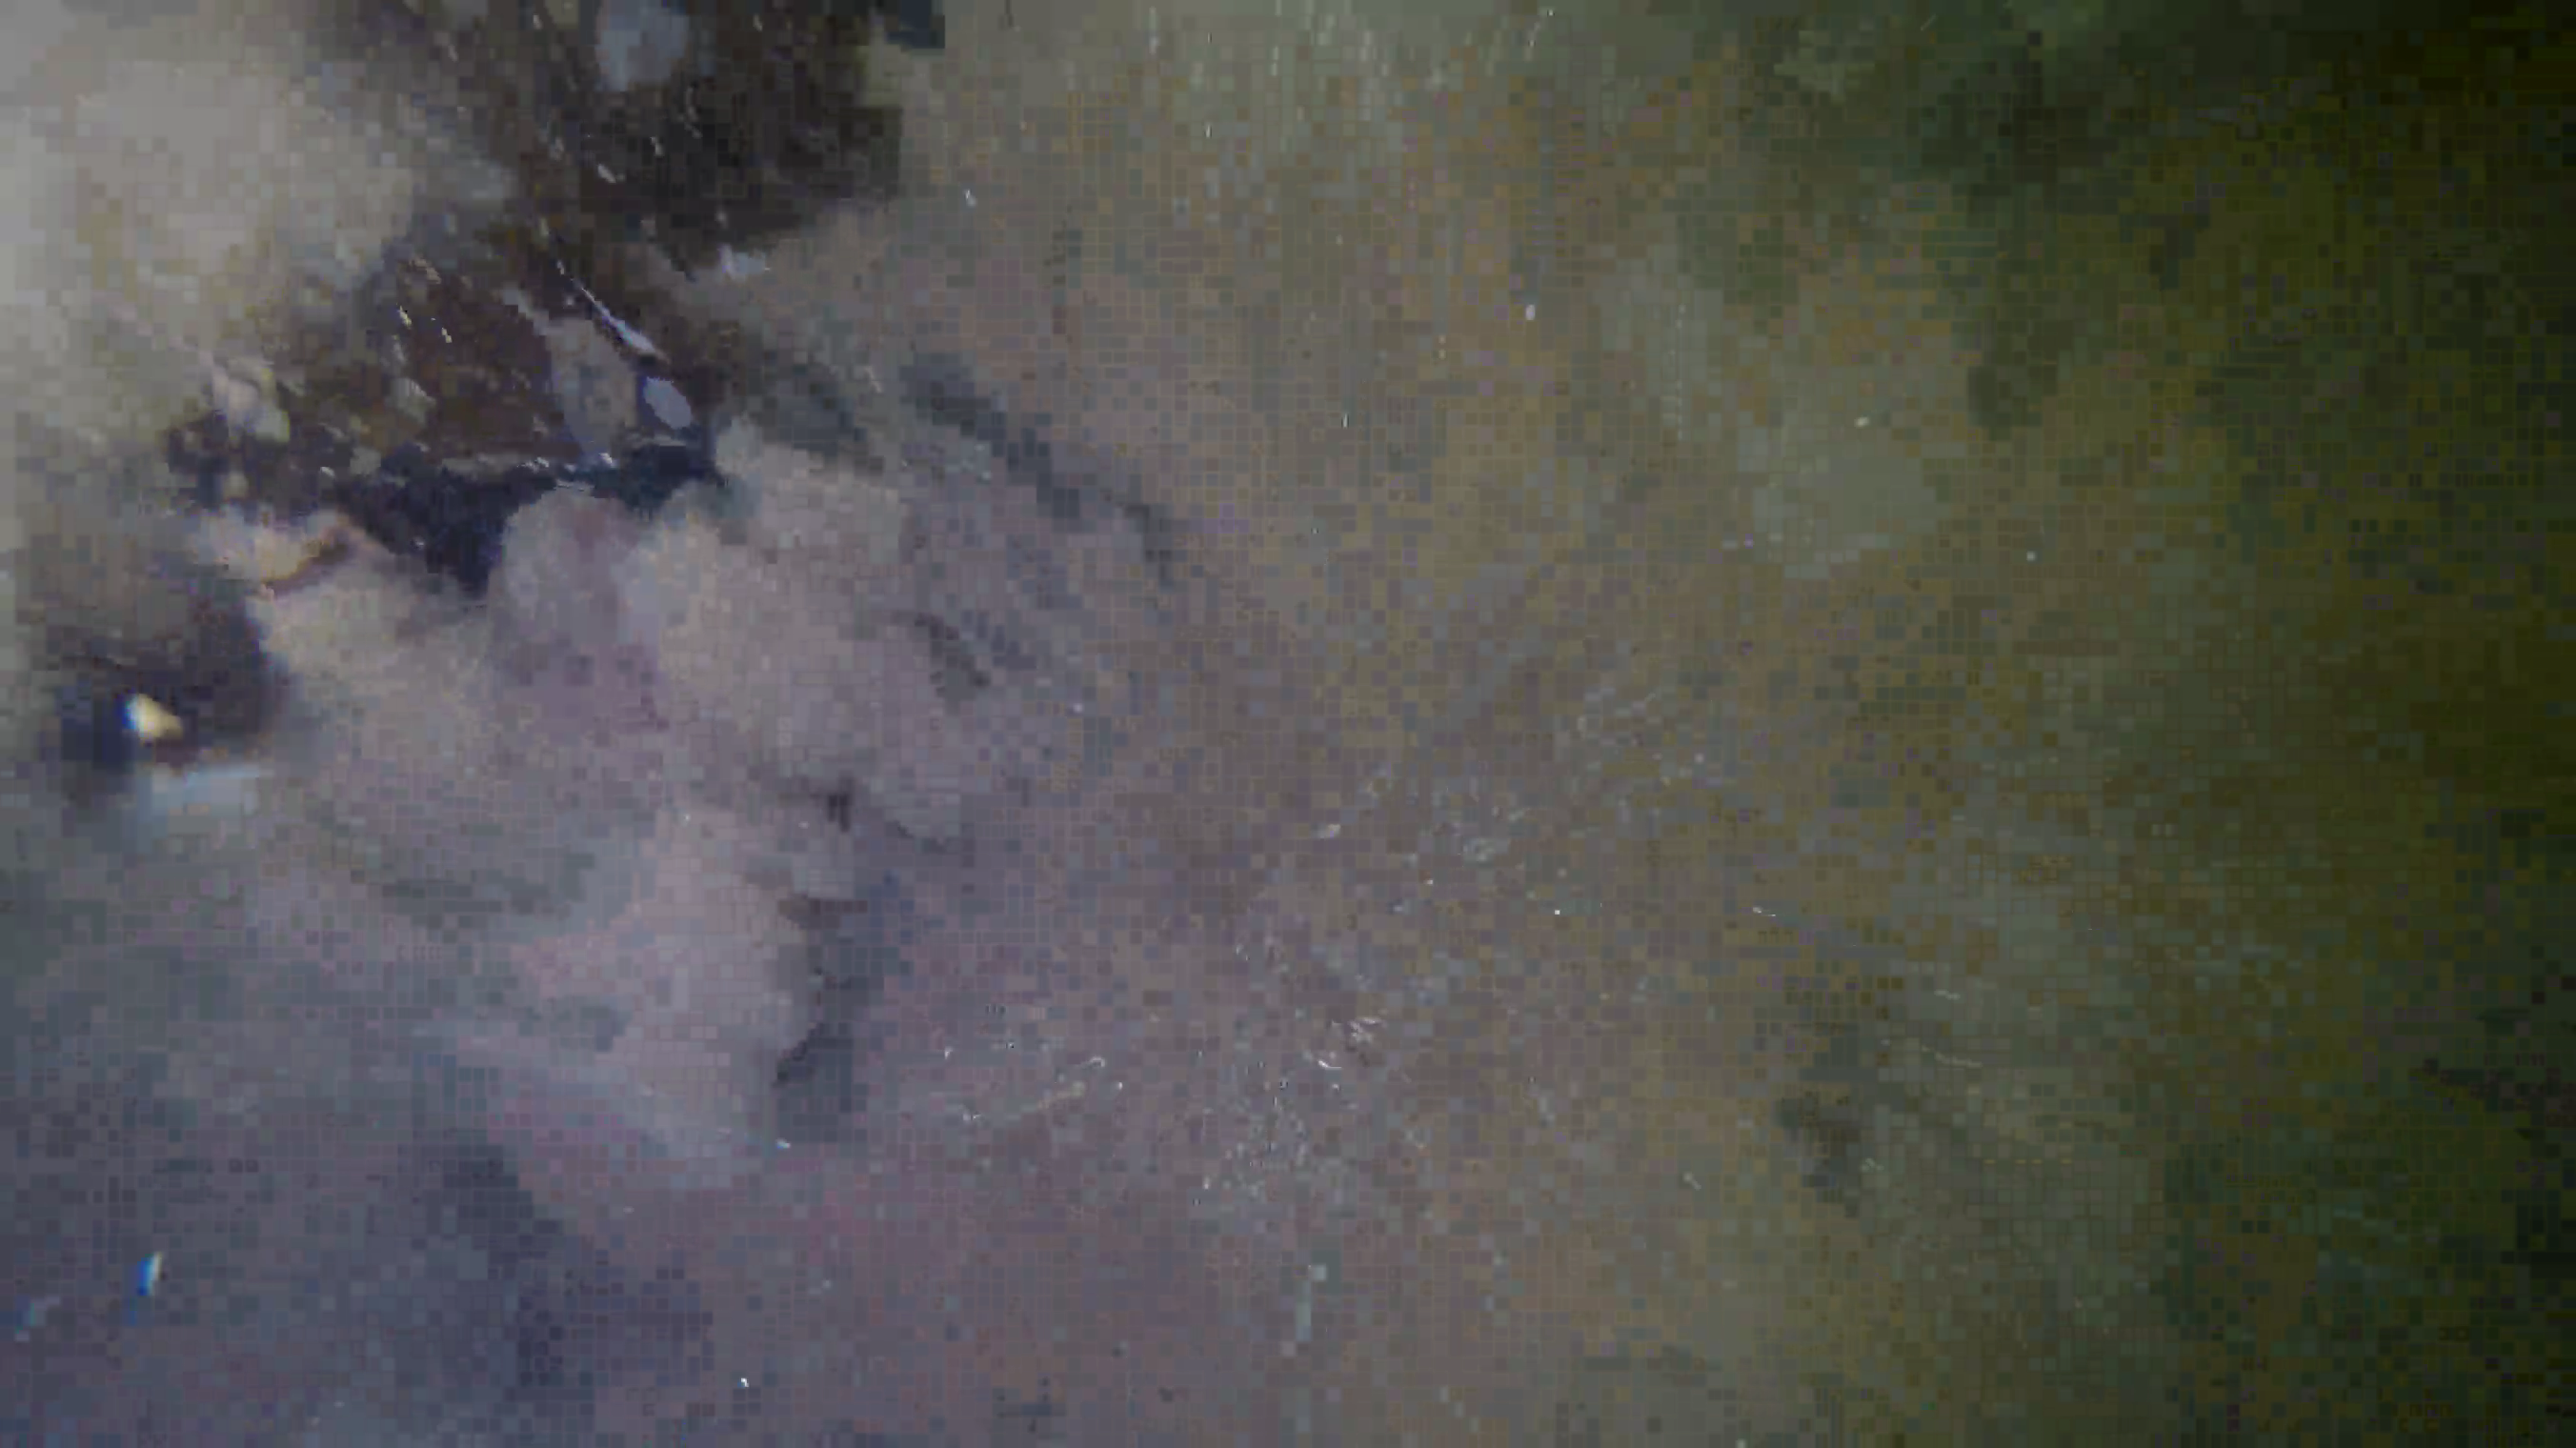
\includegraphics[width=1\linewidth]{assets/gopro_footage_artefacts.png}
        \caption{}
        \label{fig:artefacts}
    \end{subfigure}
    \caption{Frames from the GoPro footage: (\ref{sub@fig:motionblur}) showing the motion blur of backscatter particles, and (\ref{sub@fig:artefacts}) showing the pixelation artefacts (depending on your display, you may have to look closely to see the pixelation effect).}
    \label{fig:gopro}
\end{figure}

When recording in raw format, the RPi GS camera captures in full 1456x1088 sensor resolution at the maximum compatible framerate of 60 frames per second, using the native RAW10 SBGGR10 Bayer format, which utilises four channels, one red, one blue, and two green, with a 10-bit depth for each. Equation \ref{eq:raw_data_per_frame} calculates the total number of bytes per frame and Equation \ref{eq:raw_data_per_second} calculates the total number of bytes per second when recording in this raw format, where $R_w$ and $R_h$ are the resolution width and height, $D_b$ is the bit depth per channel, $N_{ch}$ is the number of channels, $F_b$ is the number of bits and $F_B$ the number of bytes per frame, $F_{rate}$ is the frame rate, and finally, $S_b$ is the number of bits and $S_B$ the number of bytes per second.

\begin{align}
    \begin{split} \label{eq:raw_data_per_frame}
        F_b & = (R_w \times R_h \times D_b \times N_{ch}) \\
        & = (1456 \times 1088 \times 10 \times 4) \\
        F_b & = \SI{63365120}{\bit} = \SI{63.36512}{\mega\bit} \\
        F_B & = \SI{7920640}{\byte} = \SI{7.92064}{\mega\byte} 
    \end{split} \\
    \notag \\
    \begin{split} \label{eq:raw_data_per_second}
        S_b & = (F_b \times F_{rate}) \\
        & = (63365120 \times 60) \\
        S_b & = \SI{3801907200}{\bit} = \SI{3.8019072}{\giga\bit} \\
        S_B & = \SI{475238400}{\byte} = \SI{475.2384}{\mega\byte} 
    \end{split}
\end{align}

The calculations reveal an approximate transfer rate of \SI{475}{\mega\byte} per second when recording the raw footage, presenting a significant data throughput requirement. It would be impossible to transfer at that data rate to the boot drive due to CPU bottlenecks, and most importantly, boot drive write-speed bottlenecks, with the drive being a USB 3.1 stick. To address this challenge, it is imperative to implement a memory buffer in RAM to temporarily store the recording data, offloading data to the boot drive only once the recording concludes ensuring the system solely reserves the CPU for recording. Additionally, employing functionality to modify resolution for downscaling and to adjust the framerate, effectively further reducing the output filesize without introducing video artefacts.

\subsection{Underwater Backscatter Cancellation System}
\label{designsystem}

The system must employ an image processing pipeline, Figure \ref{fig:processing_pipeline} illustrates this pipeline from a high-level perspective. The pipeline must begin with a greyscale filtering stage to reduce image dimensionality by categorising pixels by brightness, ensuring a single-channel output, reducing processing complexity for the subsequent pipeline stages. The next stage applies a Gaussian blur to reduce noise and small-scale variations in pixel intensities, to improve the edge detection performance such that the edge detection algorithm only detects regions of interest. Post-noise-smoothening, a histogram equalisation stage can improve the dynamic range, enhancing image contrast by redistributing pixel intensities to fully utilise the intensity range. The histogram equalisation stage can drastically improve the edge detection algorithm due to the improved contrast between objects of interest. Application of the Canny algorithm will extract all edges, ideally of the backscatter in isolation due to the previous stages, aiding in the next stage, which is backscatter segmentation. The segmentation stage will utilise a simple methodology, such as highlighting closed-loop edges, in order to isolate and pinpoint the backscatter particles.

Given Python's high-level abstraction, there is a theoretical limit to how close to real-time the system can operate. For this system, I will be targetting a total processing duration, which is the time it takes to capture the frame, apply the image processing pipeline, and finally segment the backscatter particles, of \SI{33.33}{\milli\second}, which roughly equates to a framerate of 30 FPS. Employing a parallel processing pipeline, similar to the implementations by De Charette et al. and Tamburo et al., will increase system throughput to help achieve this target. Unfortunately, The Python interpreter is not fully thread-safe and thus utilises the Global Interpreter Lock (GIL), which prevents multiple processor threads from executing at once and causing race conditions. As a result, a Python-based processing pipeline will only ever process image frames sequentially, requiring the bypass of GIL to ensure parallel processing. Figure \ref{fig:multiprocessing_pipeline} illustrates the process distribution for the parallel image processing pipeline.

\begin{figure}[H]
    \centering
    
\includegraphics[width=1\textwidth]{assets/image-processing-pipeline.png}
    \caption{Design of the image processing pipeline for the system.}
    \label{fig:processing_pipeline}
\end{figure}

\begin{figure}[H]
    \centering
    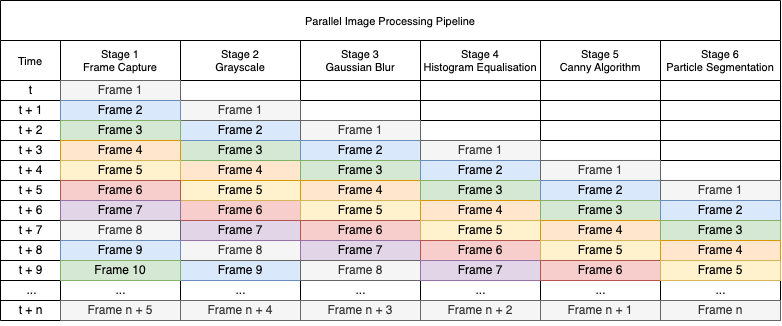
\includegraphics[width=1\textwidth]{assets/image_multiprocessing_pipeline.png}
    \caption{Design for parallel processing in the image processing pipeline for the system.}
    \label{fig:multiprocessing_pipeline}
\end{figure}

In addition to parallel multiprocessing, the system must implement a real-time kernel with the PREEMPT-RT patch. Shepherd's use of the fully-fledged Raspberry Pi OS, which includes a desktop environment and a full software suite, may have been the reason which led to its jitter, primarily due to the OS scheduler preemption type which prioritises a smoother graphical user interface over system latencies, and also due to the vast number of bundled software which could have been consuming CPU time. To ensure minimal OS and software overhead, I will be using the 64-bit Raspberry Pi OS Lite, which does not come with a desktop environment or any non-dependency software. Applying the PREEMPT-RT patch to the OS will reduce stage durations due to the reduction in system latency, and additionally, will also reduce latency randomness, ultimately improving system real-time and predictability. The final key factor is the ability to control the system frame rate, essentially by adding a delay to ensure processing at the established rate. For this design, the implementation must track the duration of each stage accurately to compute the necessary delay duration.


\section{Implementation}
\label{implementation}
Following Section \ref{design}, this section aims to implement the designs, starting with establishing remote communications with the RPi SBC, later developing toolset programs, and finally, the system itself.

\subsection{Interfacing With Raspberry Pi SBC}

Due to security reasons, also noted by Shepherd, it is not possible to connect the RPi SBC to the Eduroam University network. This incurs a major roadblock, preventing remote communication to the RPi via SSH and communications to the internet from the RPi. Two aspects will ensure complete and seamless connectivity of the system: (a) SSH connection from the laptop to the RPi to enable remote connectivity for configuration and control, and (b) internet connection from the RPi to a valid network to enable the installation and update of the OS and other software. The security policies in place across all University-owned networks block communication between devices. Therefore, there must be a separate link between the RPi and the device to initiate an SSH connection. As Figure \ref{fig:pi_interfacing} illustrates, SSH communications will occur over an Ethernet connection between the RPi and a personal computer, and internet communications will occur over Wi-Fi to a separate University of York-owned network called `mydevices', which is intended for internet access from games consoles and specific smart home devices, and can be connected to by registering the RPi SBC's MAC address via a web portal and then entering a default Wi-Fi WPA2 Personal password on the RPi.

\begin{figure}[H]
    \centering
    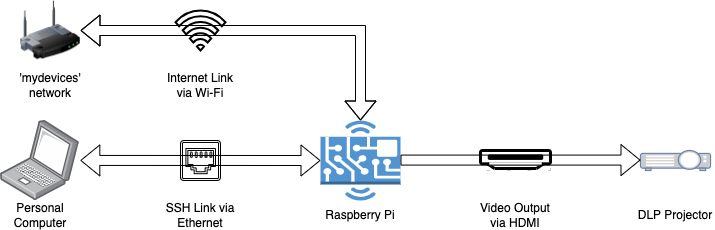
\includegraphics[width=1\textwidth]{assets/interface_diagram.png}
    \caption{The Raspberry Pi SSH and Wi-Fi communication configuration, including video output interfacing with HDMI.}
    \label{fig:pi_interfacing}
\end{figure}

The RPi must have a set hostname for easy identification, and through NetworkManager, configuring `wlan0' to connect to the `mydevices' access point for internet access, and to prevent random and intermittent SSH disconnections and unresponsiveness, configuring `eth0' to a static IP address in the format 192.168.0.xxx/24 and disabling IPv6. Creating a new network on the personal computer (PC) using the Ethernet interface with DCHP disabled, IP address set to 192.168.0.1/24, and subnet mask set to 255.255.255.0, ensures a bidirectional communication channel via Ethernet between the PC and RPi, essential for SSH. Unlike Shepherd's system, which uses the Raspberry Pi OS, this system utilises the Raspberry Pi OS Lite which lacks a desktop environment. Using SSH with X11 forwarding with an X11 display server software, such as XQuartz, on the PC, graphical user interface windows will render on the PC, enabling quick system debugging. Due to the lack of a desktop environment, video output to the DLP projector will be possible by directly writing to the Framebuffer, which is a portion of memory in RAM containing a bitmap that drives the video display output, ensuring display output rates quicker than through a GUI window such as in Shepherd's system.

\subsection{Backscatter Simulator for Synthetic Ground Truth}

This software, code in Appendix \ref{sim_code}, utilises Python 3.11.2 just like the rest of the Python programs in this project, the `Pygame' package, which is a game library, to render the graphical user interface, the `random' package to generate randomised particle velocities, the `uuid' package to generate a unique ID for each particle in the simulation, and the `csv' package to generate an export dataset consisting of the positions and radii of each particle at every simulated frame. Defining a set of constants at the start to control the simulation parameters, which Table \ref{table:simbubbleclassparams} describes, the script also consists of a `Bubble' class which denotes a backscatter particle, with the class fields in Table \ref{table:simbubbleclassfields} and the class methods in Table \ref{table:simbubbleclassfuncs}, all tables in Appendix \ref{sim_tbls}.

The program flow, illustrated in Figure \ref{fig:simflow}, begins by initialising the Pygame module and creating the graphical window and the simulation clock. If the program is not set to generate the bubble backscatter particles continuously, the program will initialise the bubble backscatter particles, ensuring that the bubble limit is reached before entering the simulation loop. Within the simulation loop, as each iteration denotes a new frame, the program initialises the simulation window background with the colour defined by the user in the constant. Next, only if the constant particle generation feature is enabled by the user, the program initialises the bubbles to the maximum count possible. Then, the program logs the position and radius of each backscatter particle in the frame before drawing every bubble and moving them. The program then runs a probability check, only if true will it randomise the velocities of every single bubble. The program then removes the particles that are outside of the simulation window before exporting an image capture of the frame. The reason behind exporting a PNG image file of each frame instead of a singular video file is to simulate the frame-by-frame capture logic of the Backscatter Cancellation System from the RPi GS Camera, Section \ref{system_impl} explains this in further detail. Finally, the Pygame-provided clock functionality limits the simulation to the user-defined constant and stores the time delta, which is the duration in seconds from the last frame, before iterating once again. When the user inputs a `quit' signal by closing the window, the program creates a CSV file, with the help of the `csv' Python module, by offloading the metric data from each frame before the program gracefully terminates.

\pagebreak
\begin{landscape}
    \begin{figure}
        \centering
        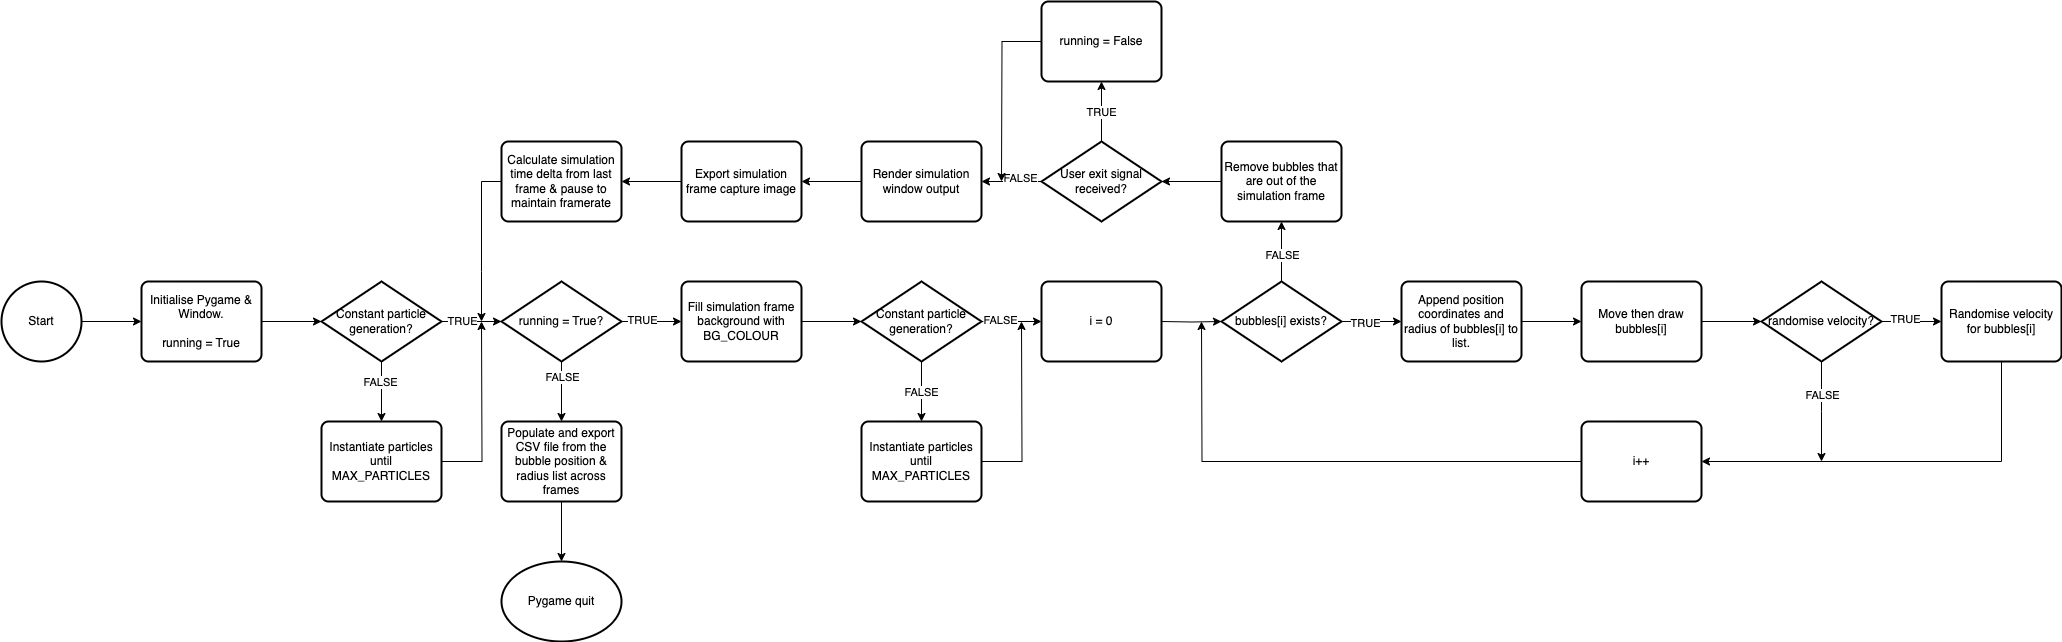
\includegraphics[width=1\linewidth]{assets/impl-sim_flow.png}
        \caption{Backscatter simulation software process.}
        \label{fig:simflow}
    \end{figure}
\end{landscape}
\pagebreak

\subsection{Lossless Video Recorder for Physical Testing}
\label{pirec_impl}

As Section \ref{designrec} introduces, this software, Python scripts in Appendix \ref{rec_code}, records test footage of bubbles from the underwater testing facility at the Institute for Safe Autonomy using an RPi 5 and an RPi GS Camera, from the submersible system itself. The software also drives a DLP projector to project a fully illuminated white light source, ensuring a well-lit scene and to induce backscatter, via HDMI using the Framebuffer to eliminate the need for a desktop environment. Aside from the main entry point script, the software consists of three self-built modules: (1) ProjectorManager, which interfaces the software with the DLP projector via the Framebuffer, (2) the CameraManager, which interfaces the RPi Camera with the software, and finally, (3) the PreviewManager, which produces the GUI window to output the recording previews and program status. The program uses the `Numpy' Python package to generate bitmap arrays of pixel values to drive the DLP projector via the Framebuffer. The `Picamera2' library, although only available as a beta release at the time of writing, provides the program with high-level access to the RPi Cameras and RPi SBC's built-in imaging hardware. The `subprocess' package spawns the FFmpeg process to encode the recording, with the assumption that FFmpeg is present on the system's RPi SBC, and finally, the program uses the `OpenCV' package to access machine-vision algorithms for image processing and to generate the preview GUI window. The tables in Appendix \ref{rec_tbls} list and describe the program configuration constants, and the fields and methods for each class.

\begin{figure}[H]
    \centering
    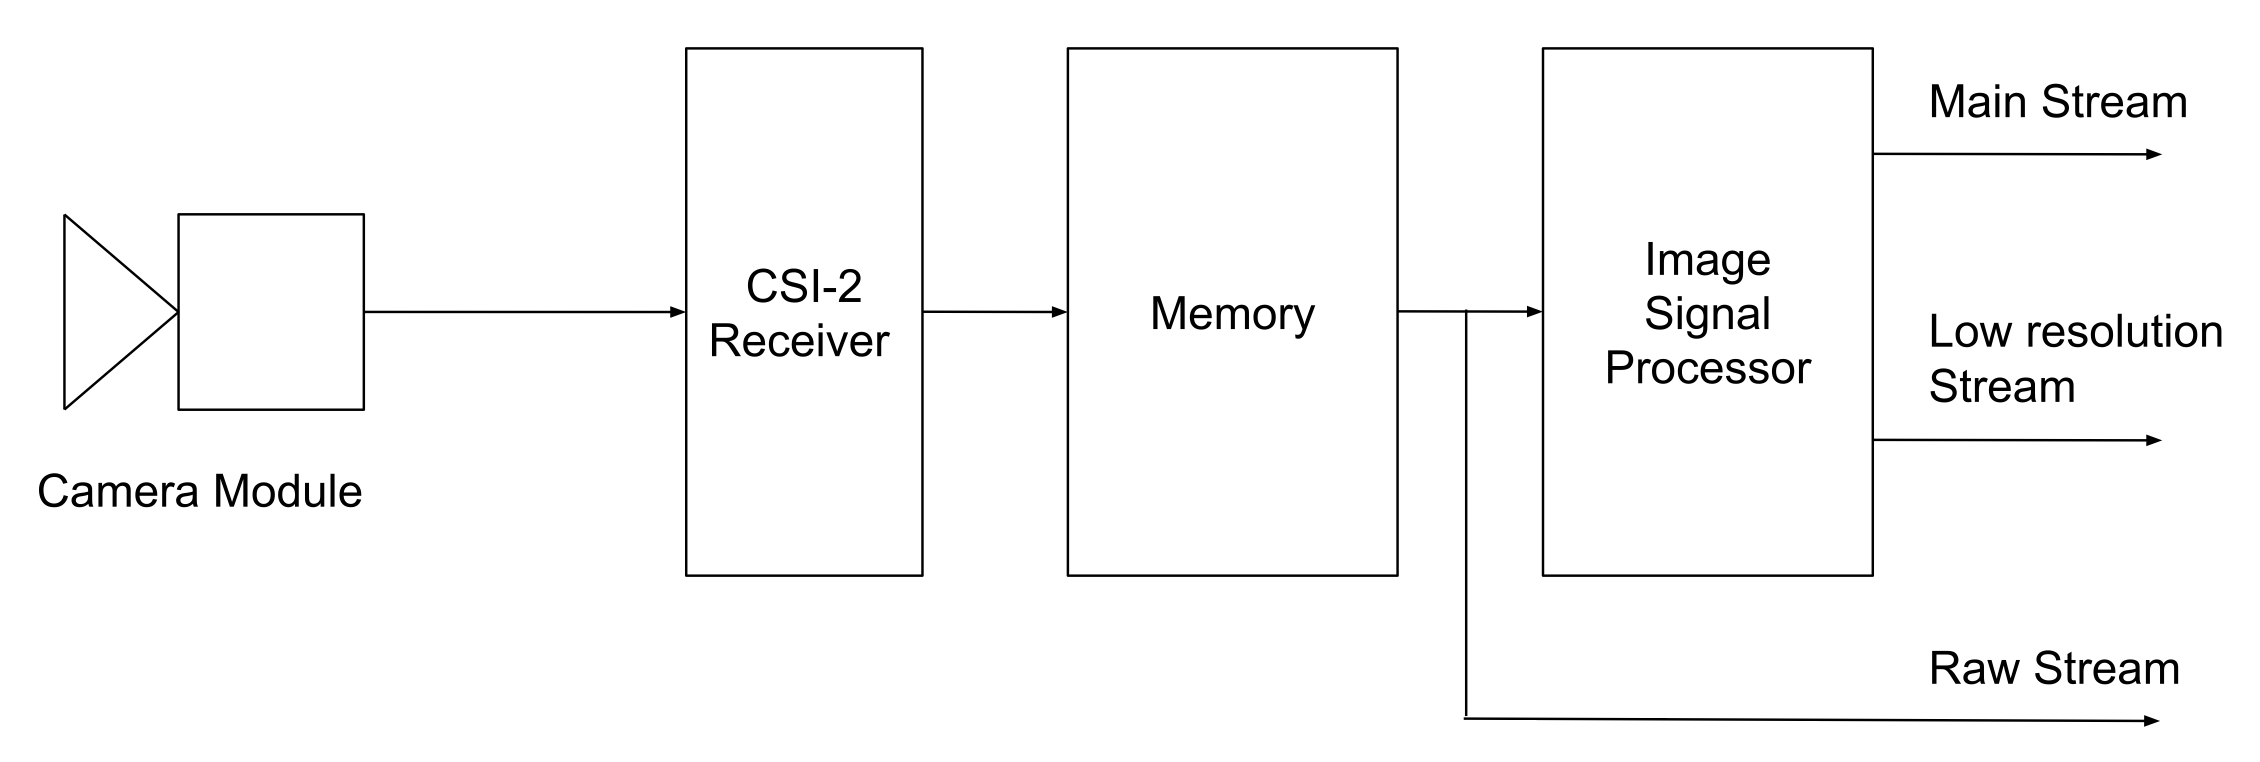
\includegraphics[width=1\textwidth]{assets/picamera-system.png}
    \caption{From \cite{raspberrypiltdPicamera2Library2024}, the Raspberry Pi camera system.}
    \label{fig:picam_system}
\end{figure}

As the Picamera2 library manual from \cite{raspberrypiltdPicamera2Library2024} illustrates, the RPi camera module delivers the output data stream, which is in native sensor format and not human-viewable, to the CSI-2 receiver hardware block onboard the RPi SBC via a ribbon cable. This hardware block transfers the incoming data into memory, ready for delivery to applications. In the initial prototyping stage for this system tool's implementation, I was receiving and recording the `raw' stream. However, this data required a lot of computationally intensive processing to convert to a human-viewable format, in addition to the high data throughput requirement of \SI{475}{\mega\byte} per second, recording at a steady rate was impossible even with a memory buffer. The Image Signal Processor (ISP) onboard the RPi SBC reads the `raw' stream from memory and efficiently cleans and processes the pixel data stream, ultimately producing a human-viewable output in either, depending on user set configuration, the RGB or YUV format. Instead of parsing the `raw' stream, I chose to process the `main' output stream in the final version of the software, configuring the exact resolution and framerates, in addition to a BGR888 output format such that the data is natively compatible with the OpenCV image processing libraries.

Figure \ref{fig:recflow} illustrates the flow of the software. The program begins with an initialisation, initialising the preview window, which passes through to the remote SSH connection on the PC via X11 forwarding, the projector via the Framebuffer, and the Picamera2 library, which applies a configuration to the RPi GS camera module and starts it. The main loop of the program then begins, retrieving the ISP-processed camera sensor array from the `main' output stream, and also retrieving the statuses of whether the projector light is on and whether the camera is recording. The sensor array frame is sent to the preview window, along with the statuses that the program overlays on the camera frame, finally logging any user-input keypresses. Using the Framebuffer, which is a memory location accessible through a directory, the program can toggle the light source by writing a bitmap array of white pixel values to turn on, and a bitmap array of black pixel values to turn off. If the program detects an `L' keypress, the projector light source toggles. With an `R' keypress, the program toggles the recording status. If the recording needs to start, the program initialises a memory buffer, configures the Picamera2 module to write to this Framebuffer along with a `Null' encoder, which ensures that the output is unencoded and `raw', and finally sends a signal to start recording. If the recording needs to stop, the program sends a signal to the Picamera2 module to stop the current recording, and using FFmpeg, which is installed on the RPi SBC, the program applies lossless encoding using the FFV1 encoder to convert the bitstream into an `.MKV' file, reducing the filesize and converting to a common video file format, for easy file transmission and so that any general-purpose software can open and this footage for playback. When the program receives an `E' key input, it will send the shutdown signal to the Picamera2 module, which gracefully terminates the camera module, it will turn off the projector light source by clearing the Framebuffer and sends a `destroy windows' signal to OpenCV which will consequently close all windows gracefully, and finally, the program exits the main loop and quits. If the program does not detect a keypress, or if it has finished handling the keypress for all inputs except the exit signal, the main loop iterates such that the entire process repeats.

\pagebreak
\begin{landscape}
    \begin{figure}
        \centering
        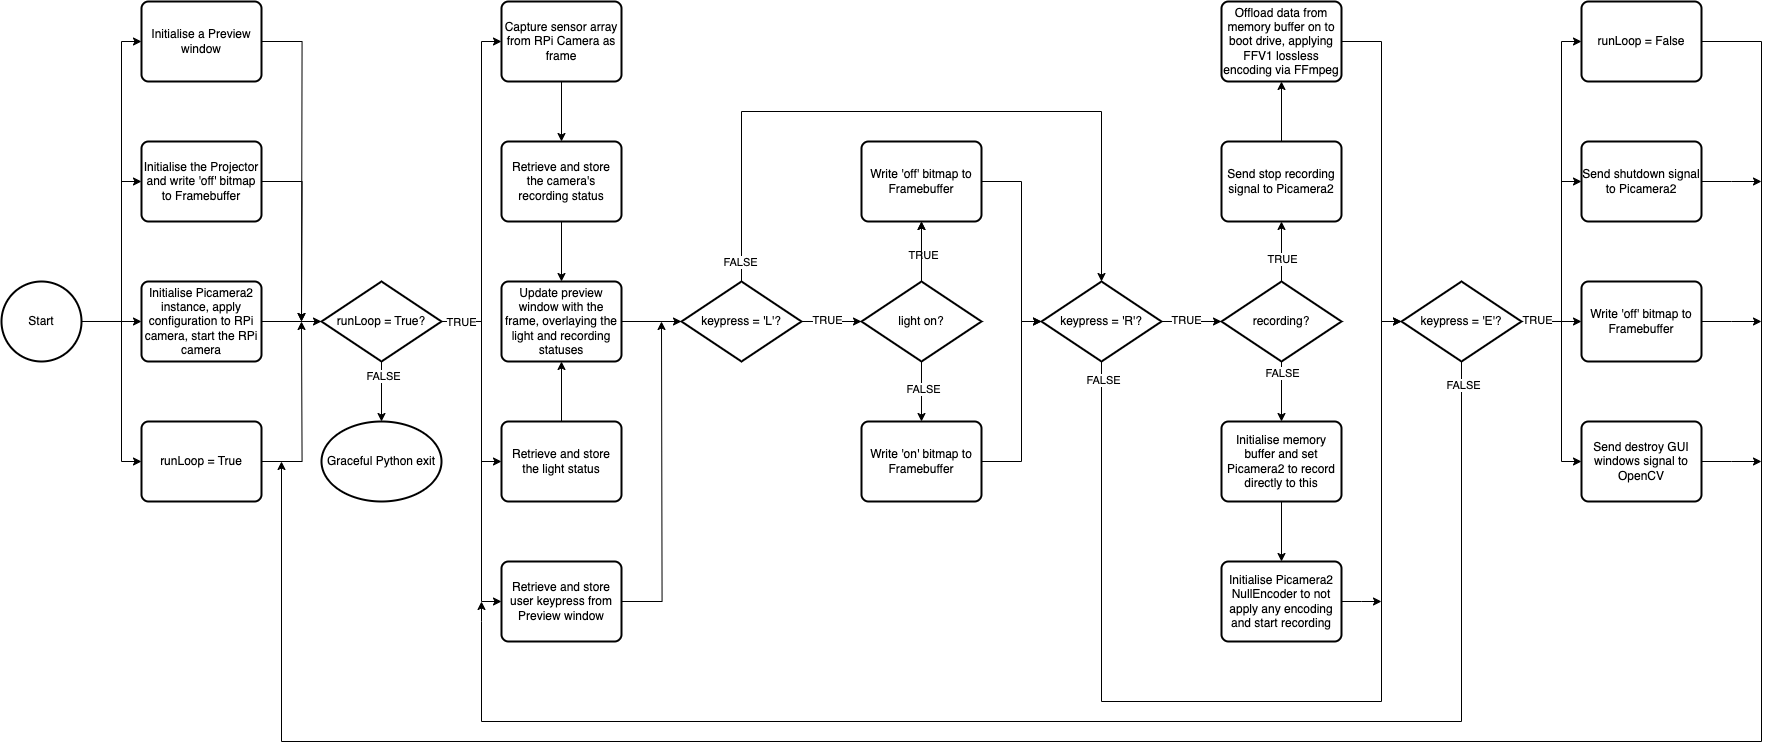
\includegraphics[width=1\linewidth]{assets/impl_rec-flow.png}
        \caption{Lossless video recorder software process.}
        \label{fig:recflow}
    \end{figure}
\end{landscape}
\pagebreak

\subsection{Underwater Backscatter Cancellation System}
\label{system_impl}

The backscatter cancellation software, as Section \ref{designsystem} describes, with code and references for methods and fields in Appendix \ref{sys}, applies an image processing pipeline to segment backscatter particle regions to then generate light patterns for selective illumination using the DLP projector. Similar to the Lossless Video Recorder implementation in Section \ref{pirec_impl}, this system follows the object-oriented paradigm for modular code, breaking down the implementation into four self-built modules, aside from the entry point: (1) CaptureManager, which contains multiple different classes for input types, for example, a Raspberry Pi Camera interface similar to the CameraManager in Lossless Recorder, and a video file stream, which allows test footage inputs. (2) BSManager, which contains the image processing pipeline and backscatter segmentation functionalities, (3) TimeManager, which contains functionality to precisely time code, and finally, (4) WindowManager, very similar to PreviewManager in the Lossless Recorder program, contains functionality to output frames to a GUI for debugging. Instead of utilising the Picamera2's recording functionality for the RPi Camera Stream class, the system captures each frame individually at each iteration so enable fine control over framerates.  Due to time constraints and issues with system offsets/parallax, which Section \ref{testing} will explain in further detail, I couldn't implement functionality to output the light patterns by directly driving the DLP projector with parallax and offset mitigation, and therefore, skipping the implementation of logic to limit the framerates, such that this system outputs entirely via the GUI windows. Just like the Lossless Recorder program, this system uses the OpenCV package for both the image processing functions and for GUI windows. The program also uses Numpy package for bitmap operations concerning the image frames, the Pandas package for large data set operations concerning the metrics that the system tracks, the `psutil' package to set the program `nice' value, which is the software priority for the OS scheduler, and finally, the `time' package, where the system harnesses the performance counter, which is a system clock with the highest available resolution, to measure code execution durations.

As Figure \ref{fig:sysflow} illustrates, the program begins by setting the software priority level, this priority level is also called the `niceness', which has the lowest compatible value of -20, denoting the highest priority, and the highest compatible value of 0, denoting lowest priority, such that the lower priority processes demands less CPU processing time and are nicer to other processes in the system. Next, the program sets the correct input stream type before initialising the graphical preview windows and entering the main system loop. Within this loop, the program captures a frame from the input stream at the start of each iteration, and for each frame, applies the image processing pipeline to segment bubbles. After a greyscale conversion, Gaussian blur, and histogram equalisation, all using OpenCV functions, the program configures the Canny edge detection algorithm following the zero-parameter approach by \cite{rosebrockZeroparameterAutomaticCanny2015}. This approach by Rosebrock, simplifies the upper and lower Canny algorithm thresholds into a single parameter, sigma, which denotes a multiplier for the median pixel intensity of the input frame, such that the upper threshold is sigma above the median, and the lower threshold is sigma below the median. While not exactly zero-parameter as Rosebrock states, as there is still a sigma parameter, this approach ensures that the edge detection adapts to the specific characteristics of the input image even in different conditions, providing effective edge maps without manual parameter tuning. The system passes the Canny output, a bitmap of detected edges, to the segmentation method which then begins by finding contours, which are curves that join all the continuous points along a boundary, using OpenCV's \texttt{findContours()} method. Next, the program sends each contour detection to OpenCV's \texttt{minEnclosingCircles()} method, calculates the smallest enclosing circle for a set of contour points, and returns the center and radii of each circle. These minimum enclosing circles (MECs) will be the black `holes' in the white light patterns, ensuring the backscatter particles are dark whilst the system fully illuminates the surrounding environment. The program renders all of the output image frames, including those from the intermediate image processing pipeline stages if the debug window option is `True', whilst logging the user-input keypresses. If the user enters the `E' key, the program breaks from the main loop and enters the shutdown sequence. The program tracks the execution duration of each image processing stage with the performance counter for each frame, including metrics on the number of MEC detections, and the total frame processing time. When the program reaches the shutdown sequence, it extracts all of the metrics and generates a CSV export file, then exits all GUI windows, sends a shutdown signal to the RPi camera module, and finally exits completely.

\pagebreak
\begin{landscape}
    \begin{figure}
        \centering
        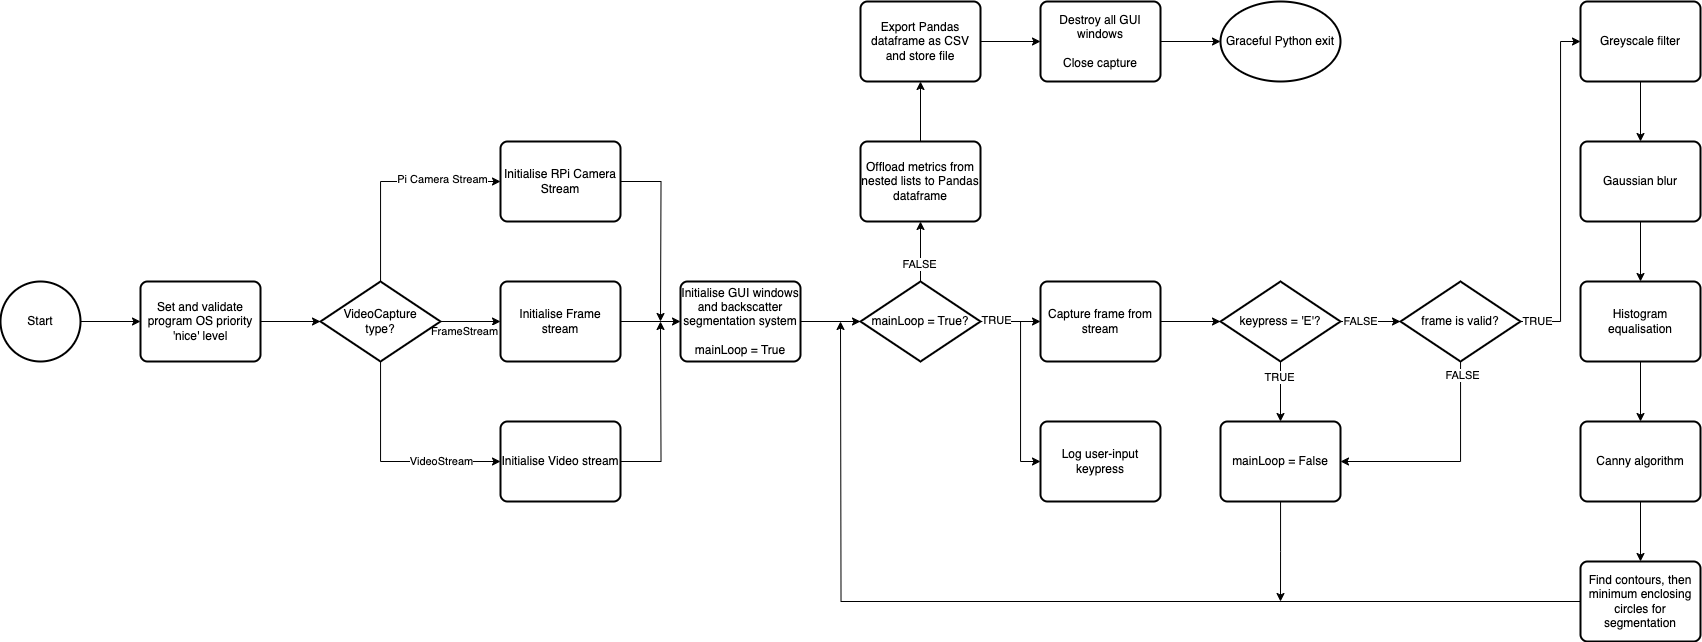
\includegraphics[width=1\linewidth]{assets/impl_system-flow.png}
        \caption{Backscatter cancellation system software process.}
        \label{fig:sysflow}
    \end{figure}
\end{landscape}
\pagebreak

\subsubsection{Implementing Multiprocessing}

The functionality of the multiprocessing system follows very closely to the aforementioned base system, which only utilises a single thread due to the Python GIL limitations. Appendix \ref{mpsys} contains the references for methods and fields as well as the code for this implementation. The `multiprocessing' Python package provides an interface to support spawning subprocesses with concurrency, effectively side-stepping the GIL, and ultimately enabling the system to fully leverage multiple processors on a given machine, unlike Shepherd's system which employs `multithreading' and, therefore, is subject to the GIL for standard CPython execution. The single-thread version of the system is split into eight stages, denoted by classes that inherit the `multiprocessing' Process, which is an object that spawns as a separate process: (1) Capture, which first initialises the input stream, then enters an infinite loop that iterates until the input stream ends whilst returning the capture frame and any user-input keypresses. (2) Greyscale, which simply applies the greyscale filter. (3) Histogram Equalisation, which also simply applies histogram equalisation. (4) Gaussian Blur, again simply applying a Gaussian blur. (5) Canny Algorithm, which applies the Canny edge detector using the `zero-parameter' approach by Rosebrock. (6) Segmentation, which first finds the contours before applying the minimum enclosing circle function to segment the bubbles. (7) Project, which originally intended to output the light patterns to the Framebuffer, however due to the aforementioned constraints and limitations, instead outputs to a graphical preview window. Finally, (8) Logging, which exports the metrics into a Pandas DataFrame, then into a CSV document.

Due to the asynchronicity of the processes, the system employs queues to send data between stages in a thread-safe manner, preventing instances of data corruption with shared memory locations such as standard variables due to clobbering, where a process overwrites data while another was reading the data. The Capture stage will start filling its output queue with frames, and if no frames are left, or if the process receives a `quit' signal from the user, it enqueues with a special code instead of a frame. This queue is input to the next stage, which is Greyscale, and this stage begins to dequeue, applying the greyscale filter, then enqueues to its output queue, and if it receives a quit code instead of a frame, it will shutdown itself after forwarding the code. This logic repeats across all the other stages.

\subsection{Applying the PREEMPT-RT Patch}

The latest version of Raspberry Pi OS Lite at the time I built the real-time kernel used the 6.6.20 Linux kernel version. Therefore, I applied the PREEMPT-RT patch with the corresponding version label of 6.6.20-rt25. While building, I selected the `Fully Preemptible Kernel (Real-Time)' option, also enabling the RCU priority boosting with a \SI{500}{\milli\second} delay boosting for the RT kernel and enabled the `Multi-core scheduler support' option for both RT and the non-RT kernels.

\section{Testing \& Evaluation}
\label{testing}
In previous work, Shepherd employs a five-stage testing method: (1) calibration for parallax mitigation, (2) testing stationary backscatter, (3) testing with different reflective materials inducing backscatter, (4) motion and synchronisation of the system, and (5), underwater testing. Shepherd carries out these tests using a temporary testing rig, outside the submersible system, consisting of the projector, camera and RPi SBC fastened to a wooden plate, and employing the submersible system with the end open for underwater testing by partial submersion in a water barrel. Unfortunately, due to the large offsets and parallax between the camera and projector, the project shifts its focus from physical testing to software testing and real-time performance analysis. Following the details on implementation in Section \ref{implementation}, this section aims to describe the testing process for testing both the system and the toolsets, including an evaluation of the backscatter cancellation system performance.

\subsection{Testing the Systems}

\subsubsection{Bubble Backscatter Simulator}

The bubble backscatter simulator program works very well as a simple backscatter simulation. As Figure \ref{fig:sim_validate} illustrates, the program successfully renders a preview graphical user interface, enabling the user to view the bubbles as they generate and move, and the program also correctly exports each frame of the simulation as a PNG file, emulating the frame-by-frame capture loop behaviour of the backscatter cancellation system. Furthermore, the program exports a CSV dataset of the individual backscatter particle positions and radii from each frame, classing each particle with a unique ID, for the first few particles in the dataset. Despite this, a major drawback that I found from this program is the fact that it doesn't simulate varying backscatter appearances, such as morphological transformations with shape warping, and colour changes, to verify if the system can detect varying backscatter parameters, as all particles are exactly circular and white. In addition, the program does not simulate varying background conditions as the background is exactly black, resulting in the inability to verify whether the system can correctly isolate and segment just the particles and not any regions of interest in the background.

\begin{figure}[H]
    \centering
    \begin{subfigure}{.49\textwidth}
        \centering
        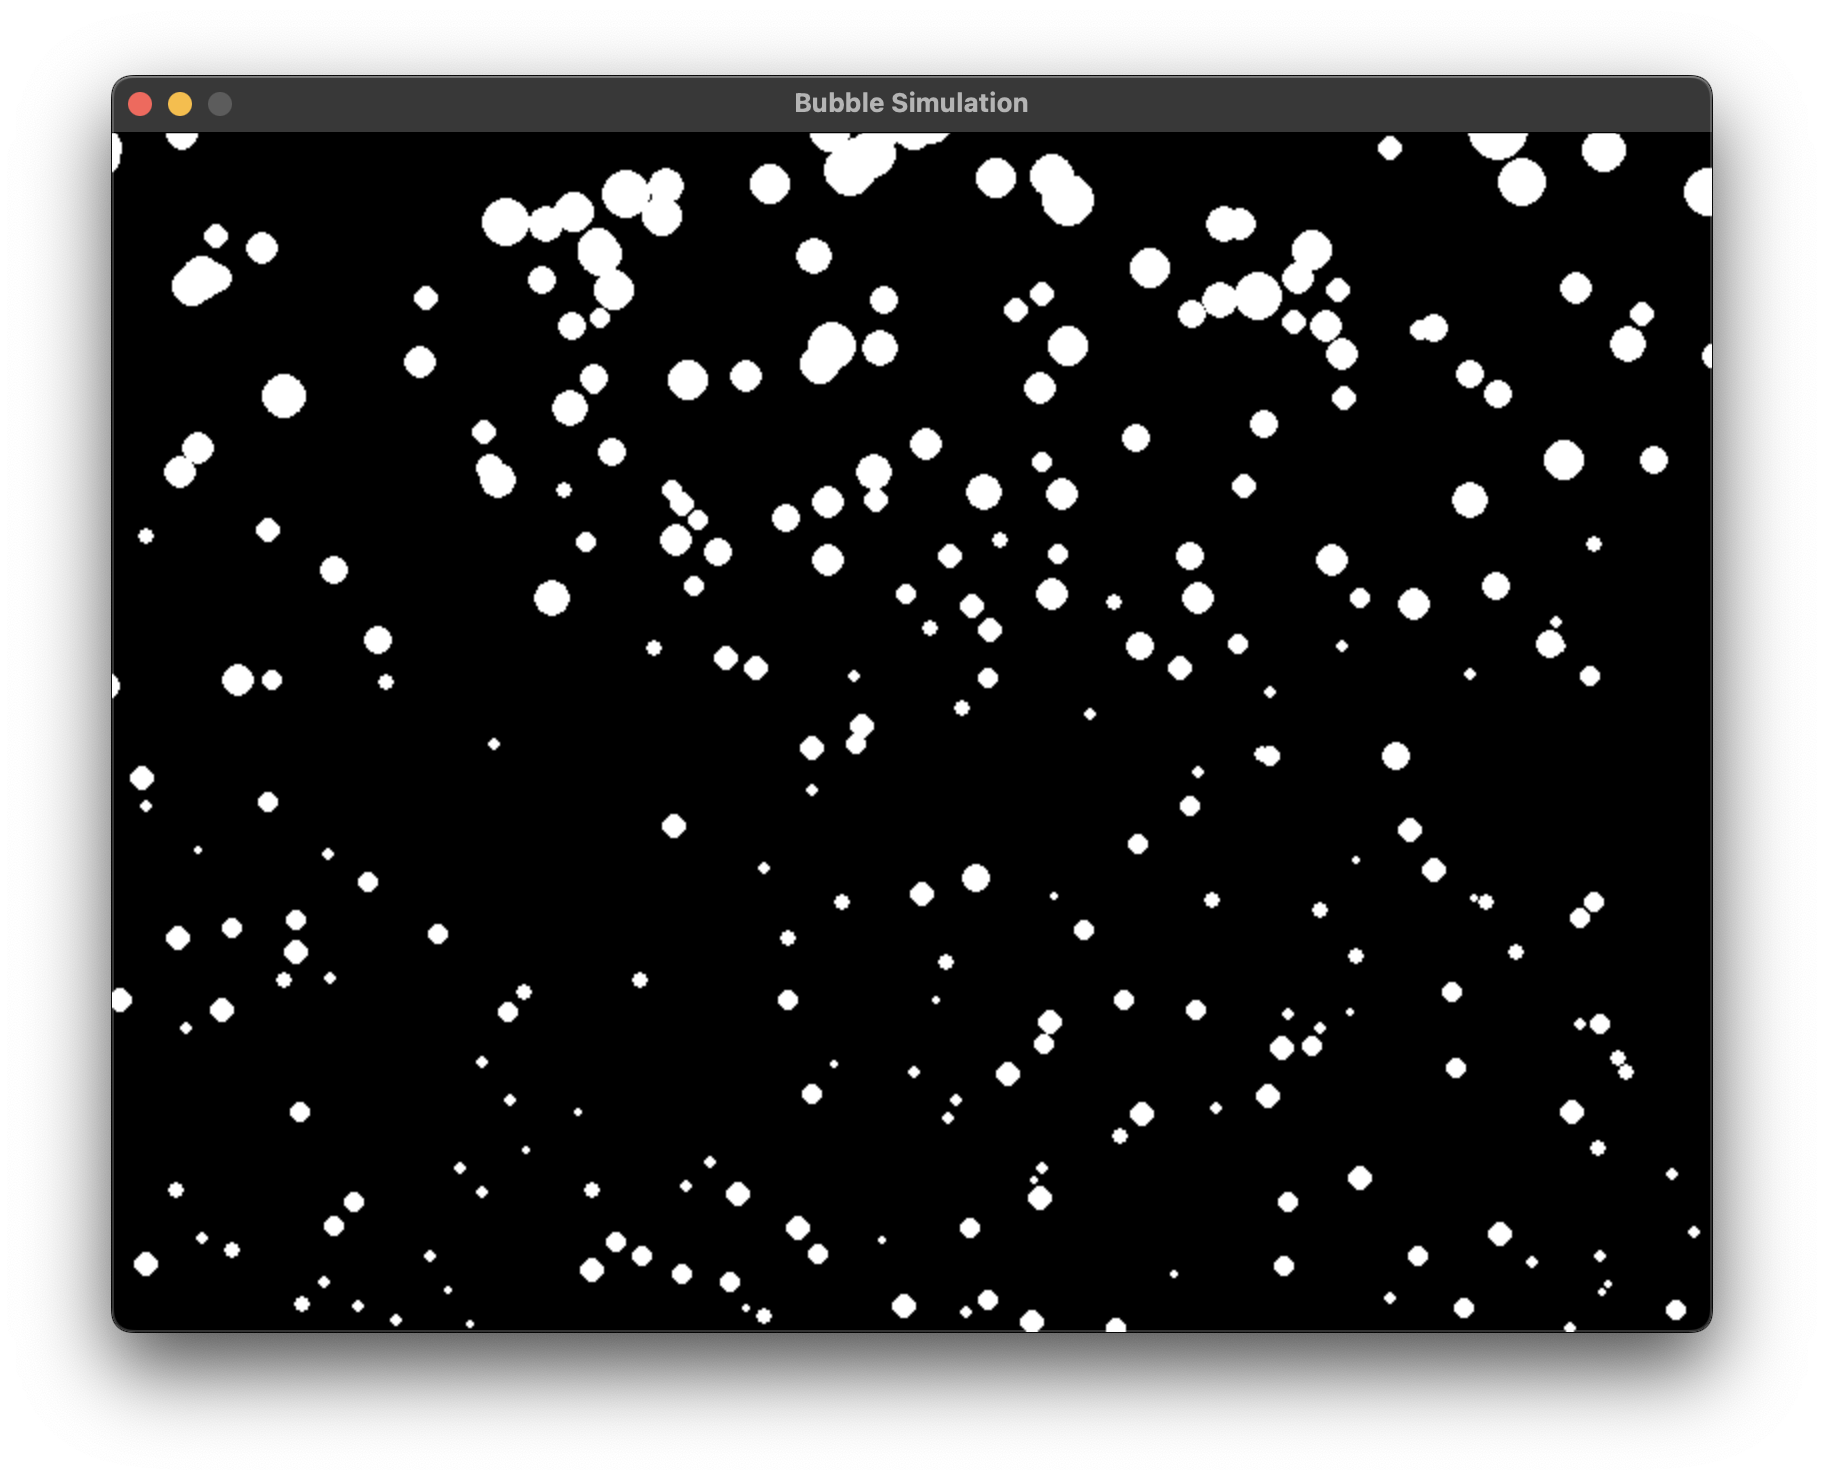
\includegraphics[width=1\linewidth]{assets/test-sim-sc.png}
        \caption{}
        \label{fig:sim_sc}
    \end{subfigure}
    \hfill
    \begin{subfigure}{.49\textwidth}
        \centering
        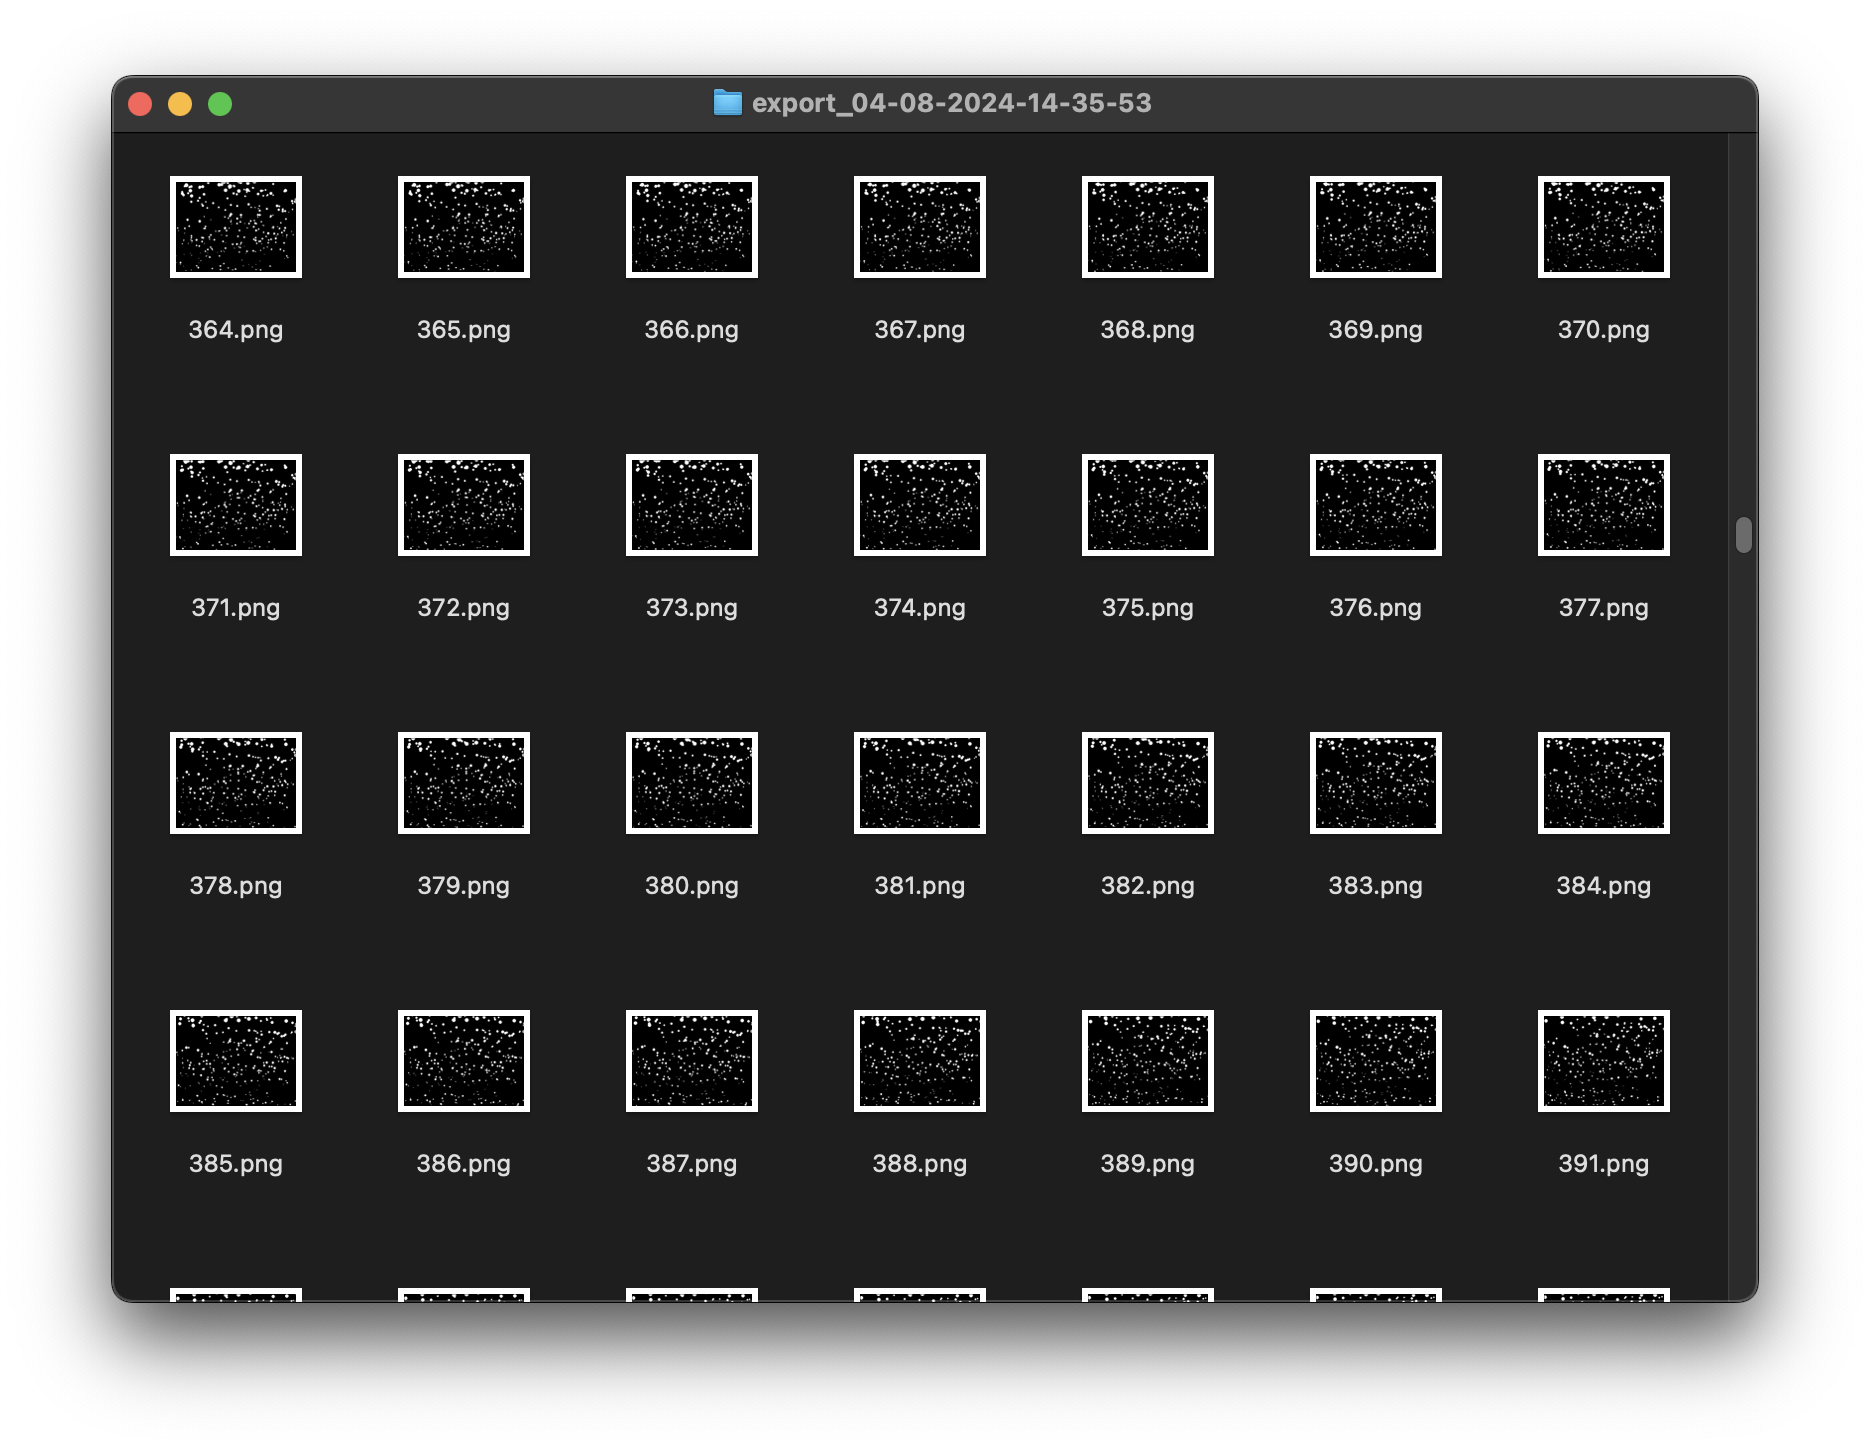
\includegraphics[width=1\linewidth]{assets/test-sim-frames.png}
        \caption{}
        \label{fig:sim_frames}
    \end{subfigure}
    \caption{Screenshots validating the Bubble Backscatter Simulator program: (\ref{sub@fig:sim_sc}) showing the preview GUI window, and (\ref{sub@fig:sim_frames}) showing the list of frames in the output directory.}
    \label{fig:sim_validate}
\end{figure}

\subsubsection{Lossless Video Recorder}
The lossless video recorder proved an invaluable tool that performed almost flawlessly, as Figure \ref{fig:rec_validate} illustrates. A change I had to make was to modify the OS to ensure the console would not output to the HDMI Framebuffer, as this was causing interference with my Framebuffer-driven light source. Unfortunately, as the figure also illustrates, there was a major misalignment issue, where the camera is only able to a small corner in the bottom-left of the projector-lit scene. While a simple cropping function can resolve most of this, which I have implemented in the backscatter cancellation system, albeit reducing the system's useable region, the system will still be affected by the camera's internal reflection, which reduces the field of view and adds distortion. Nevertheless, the recordings were very helpful in verifying the system in a non-synthetic environment without requiring re-deployment underwater.

\begin{figure}[H]
    \centering
    \begin{subfigure}{.49\textwidth}
        \centering
        \includegraphics[width=1\linewidth]{assets/underwater-testing.png}
        \caption{}
        \label{fig:underwater}
    \end{subfigure}
    \hfill
    \begin{subfigure}{.49\textwidth}
        \centering
        \begin{subfigure}{\textwidth}
            \centering
            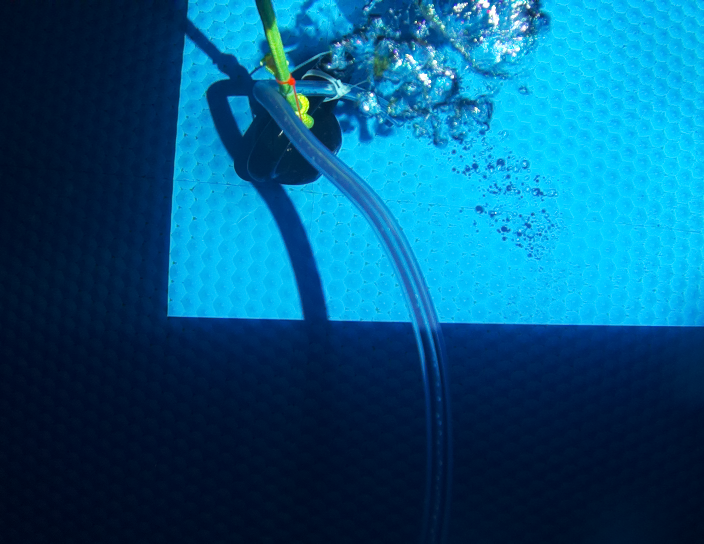
\includegraphics[width=1\linewidth]{assets/rec-frame.png}
            \caption{}
            \label{fig:rec_frame}
        \end{subfigure}
        \vfill
        \begin{subfigure}{\textwidth}
            \centering
            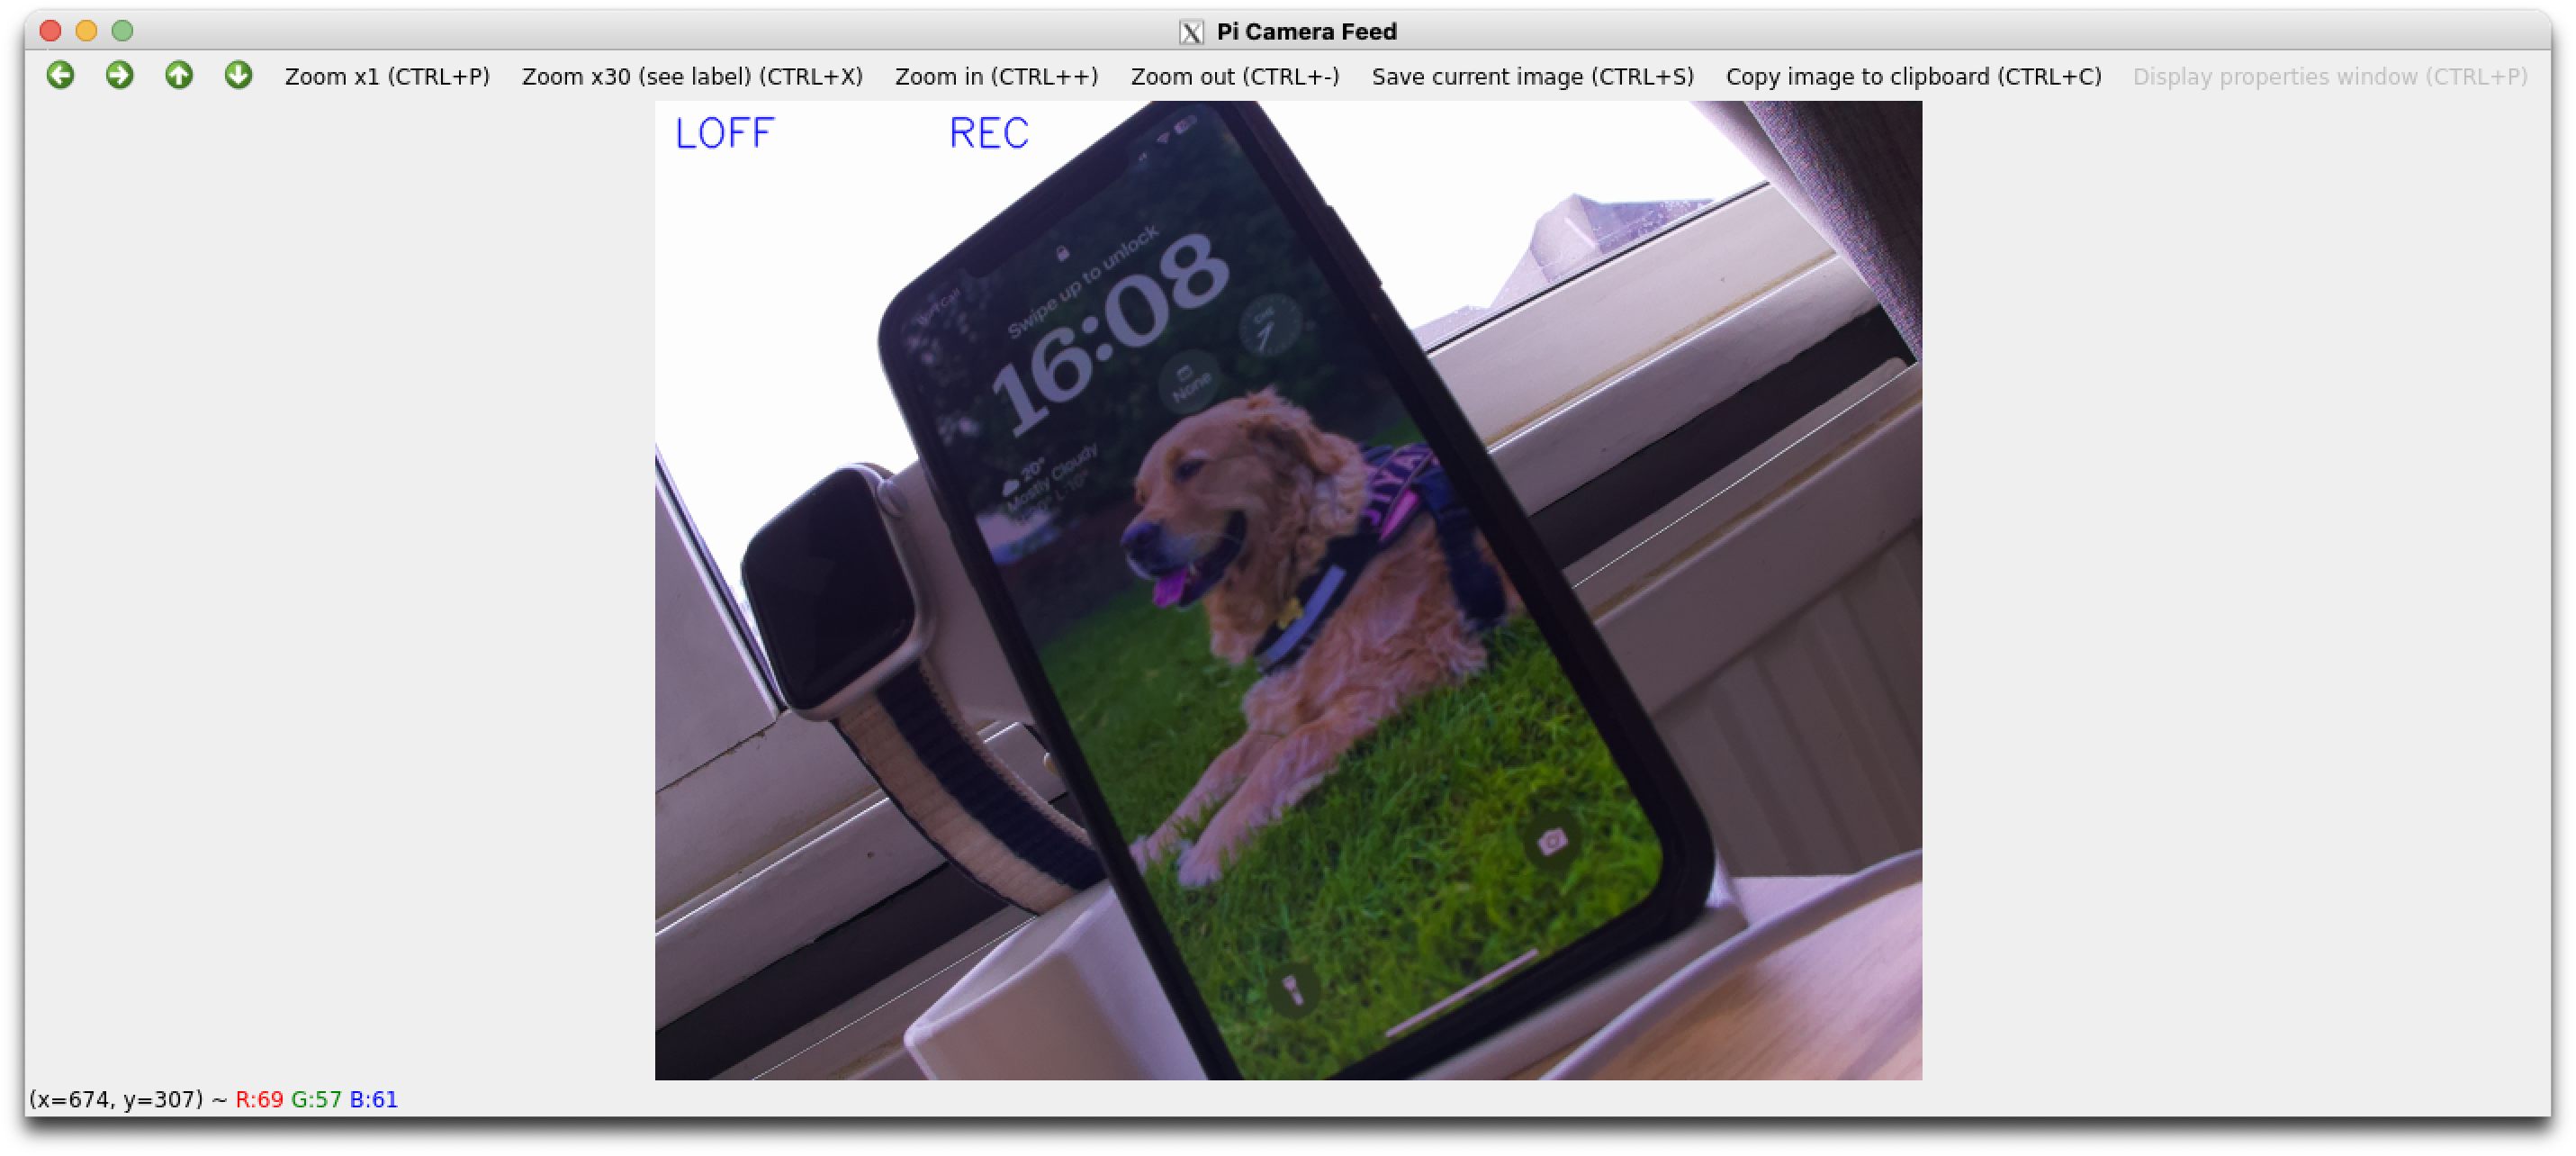
\includegraphics[width=1\linewidth]{assets/rec_sc.png}
            \caption{}
            \label{fig:rec_sc}
        \end{subfigure}
    \end{subfigure}
    \caption{Figures validating the Lossless Video Recorder program: (\subref{fig:underwater}) showing the submersible recording underwater at the Institute for Safe Autonomy testing tank, (\subref{fig:rec_frame}) an extracted frame from recorded footage, and (\subref{fig:rec_sc}) showing the preview GUI window, rendered remotely with X11 forwarding.}
    \label{fig:rec_validate}
\end{figure}

\subsubsection{Backscatter Cancellation System}
I first verified the backscatter cancellation system using the output from the backscatter simulation and it worked flawlessly, identifying and segmenting the bubbles correctly using the minimum enclosing circle logic, as Figure \ref{fig:sys_sim} illustrates. However, when using the underwater test footage, the system started to incorrectly detect the background, mainly the textured padding of the testing tank, as Figure \ref{fig:sys_histequ} illustrates. I identified that this was caused by the histogram equalisation stage, where the entire image frame's pixel intensities are spread, increasing the contrast substantially. I therefore replaced this stage with an OpenCV binary thresholding implementation, ensuring that the system only passes certain pixel intensities. The results after this processing pipeline stage replacement were much better, as Figure \ref{fig:sys_binth} illustrates. Figure \ref{fig:sys_flow_visual} illustrates the final system's image processing pipeline flow.

\begin{figure}[H]
    \centering
    \begin{subfigure}{.48\textwidth}
        \centering
        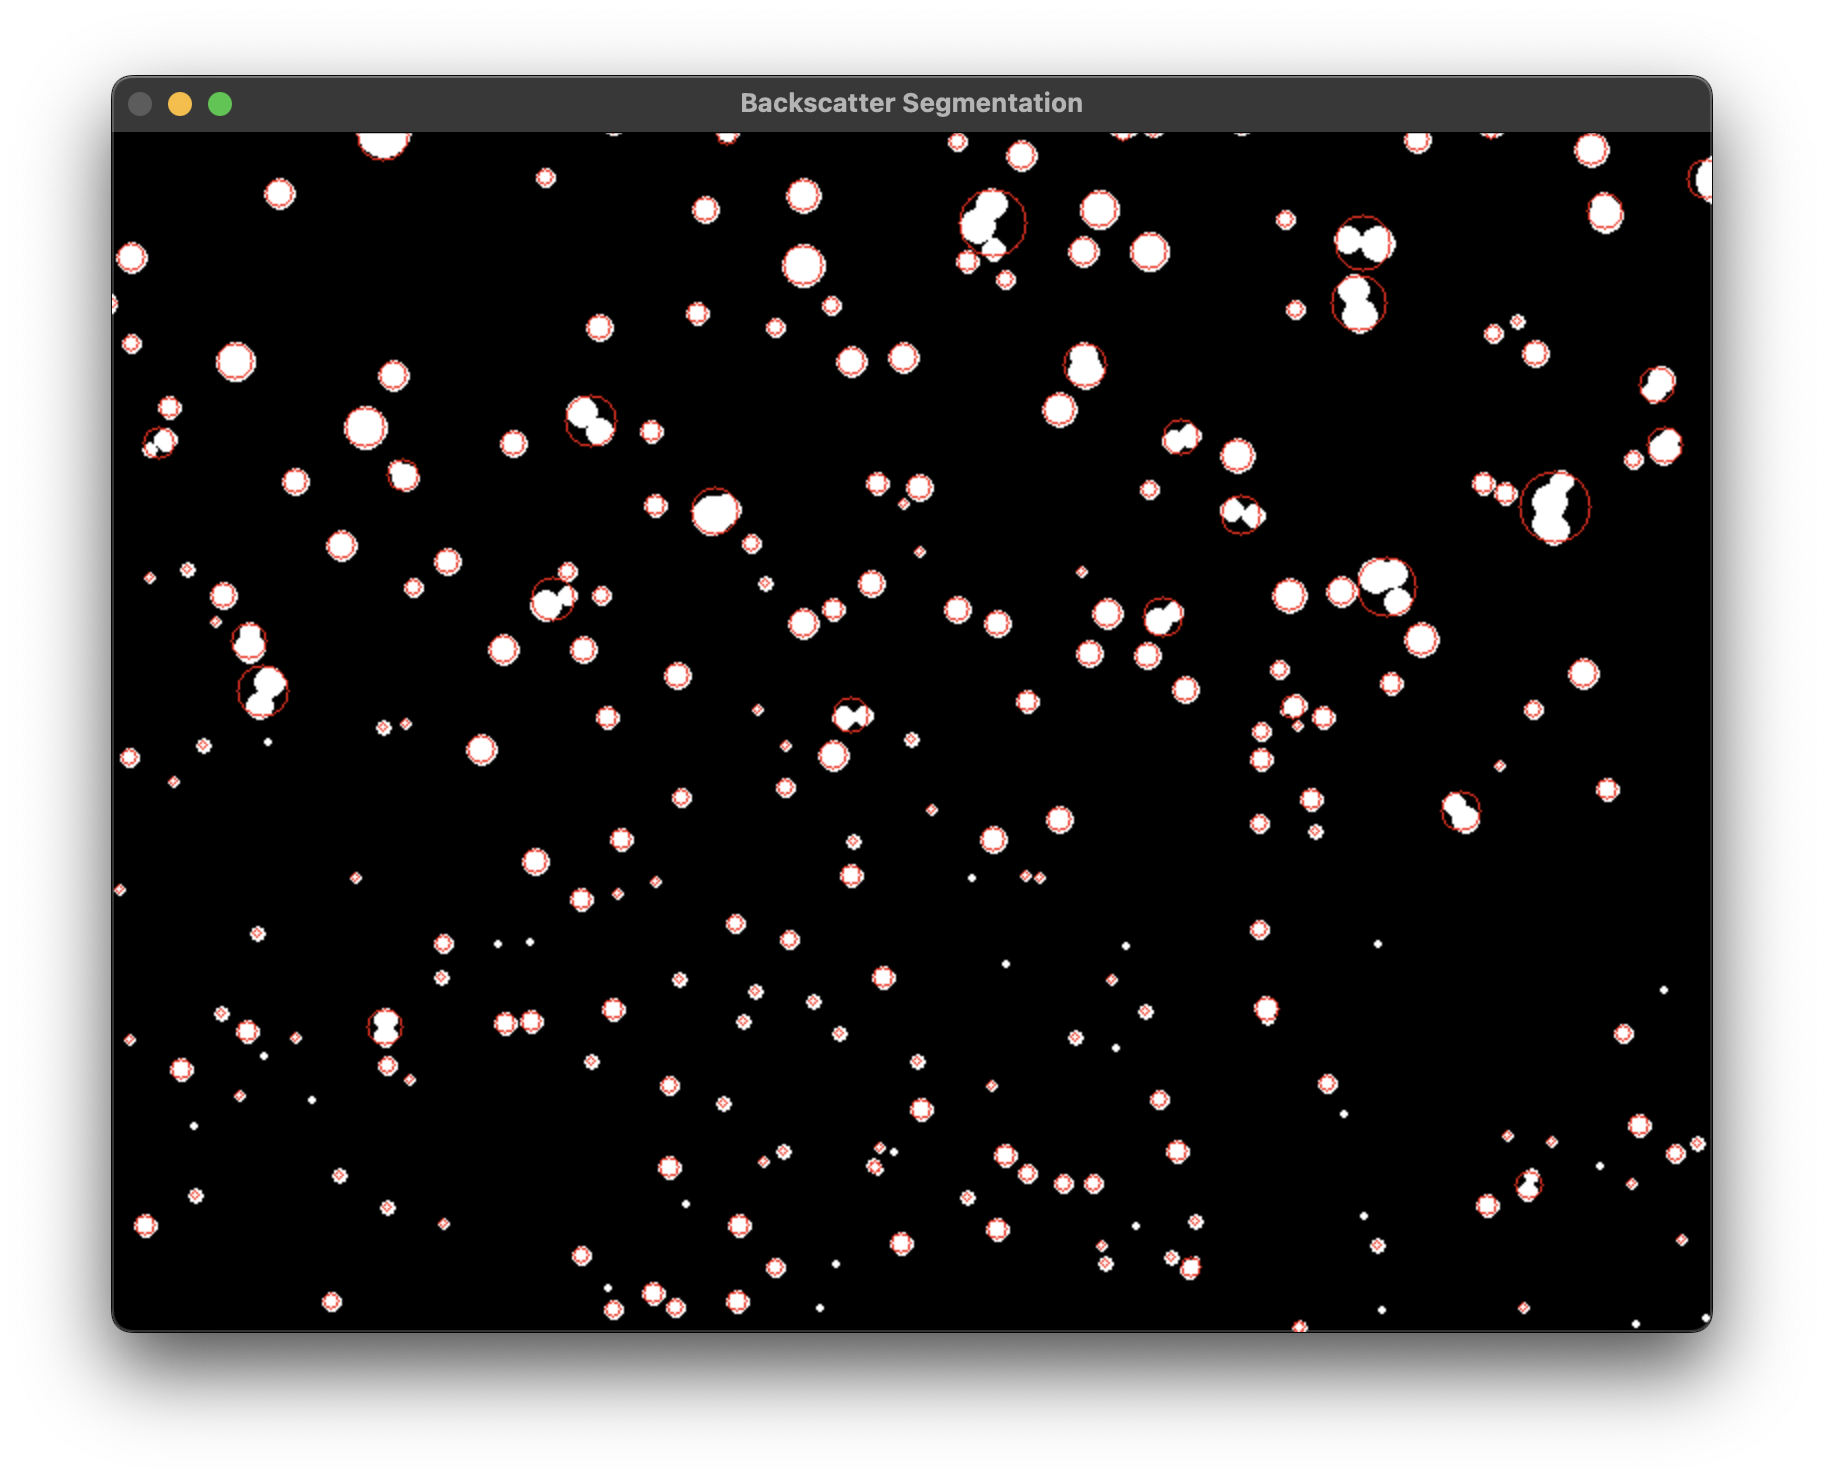
\includegraphics[width=1\linewidth]{assets/sys_sim.png}
        \caption{}
        \label{fig:sys_sim}
    \end{subfigure}
    \hfill
    \begin{subfigure}{.25\textwidth}
        \centering
        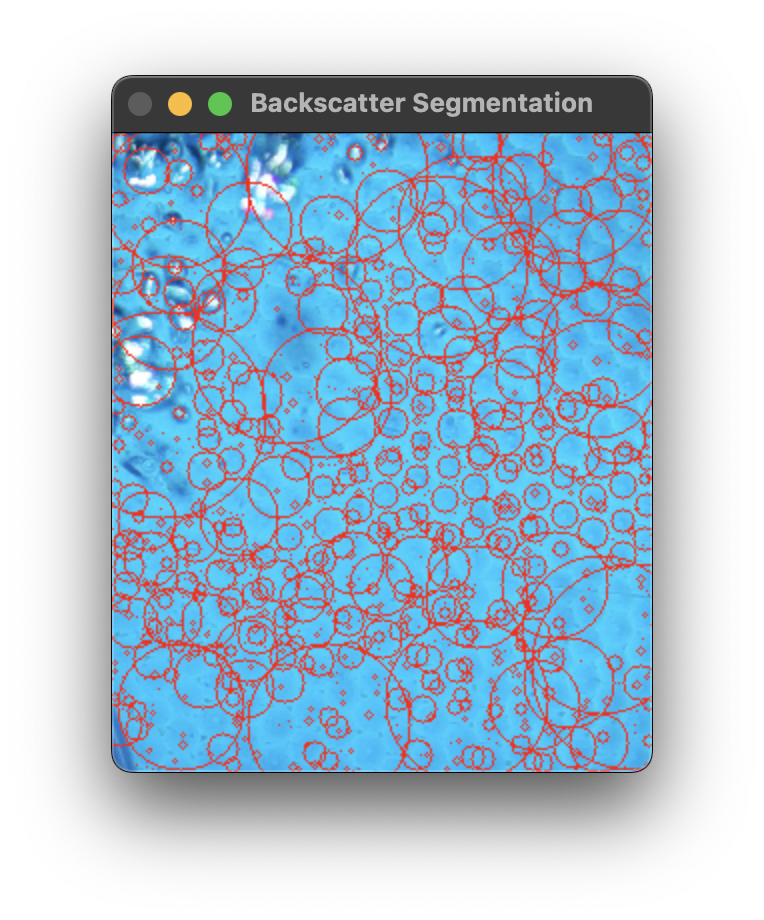
\includegraphics[width=1\linewidth]{assets/sys_histequ.png}
        \caption{}
        \label{fig:sys_histequ}
    \end{subfigure}
    \hfill
    \begin{subfigure}{.25\textwidth}
        \centering
        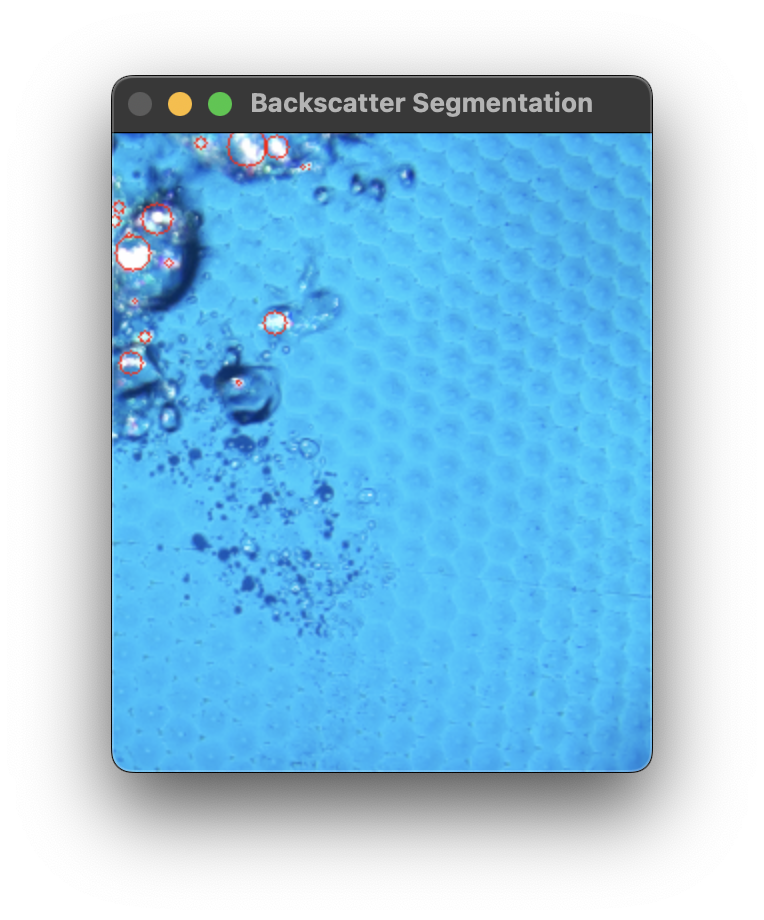
\includegraphics[width=1\linewidth]{assets/sys_binth.png}
        \caption{}
        \label{fig:sys_binth}
    \end{subfigure}
    \caption{Screenshots validating the Backscatter Cancellation System program: (\ref{sub@fig:sys_sim}) showing the backscatter segmentation (red circles) from the Backscatter Simulator output, (\ref{sub@fig:sys_histequ}) incorrect segmentation of backscatter from the test footage, and (\ref{sub@fig:sys_binth}), which shows the correct backscatter segmentation using the same footage.}
    \label{fig:sys_validate}
\end{figure}

\begin{figure}[H]
    \centering
    \begin{subfigure}{.6\textwidth}
        \begin{subfigure}{0.32\textwidth}
            \centering
            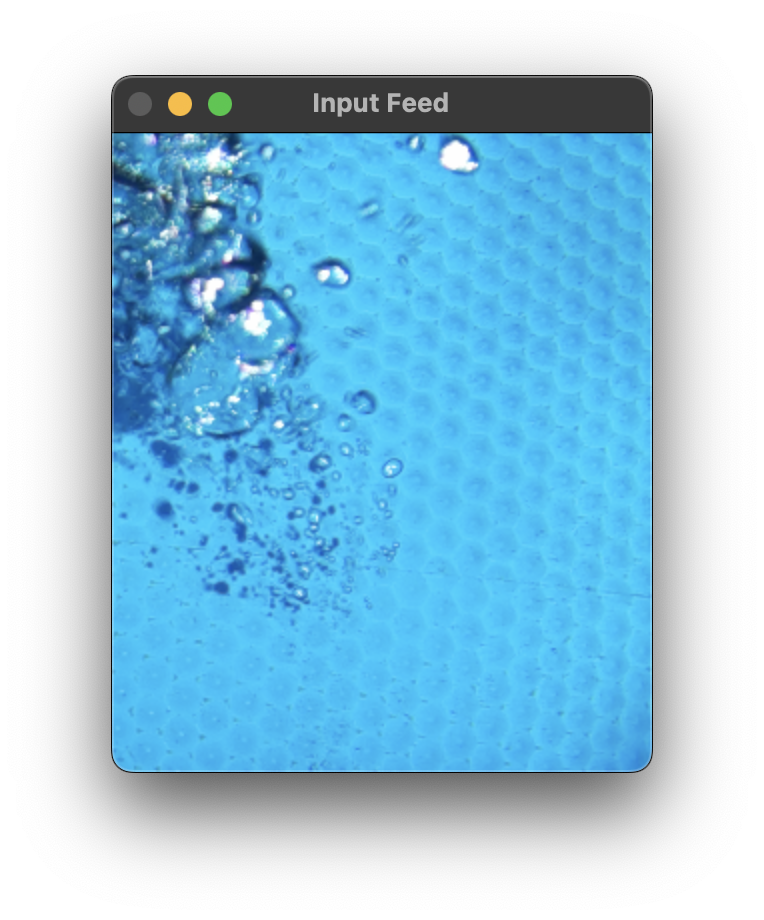
\includegraphics[width=1\linewidth]{assets/sys_input.png}
            \caption{}
            \label{fig:sys_input}
        \end{subfigure}
        \hfill
        \begin{subfigure}{0.32\textwidth}
            \centering
            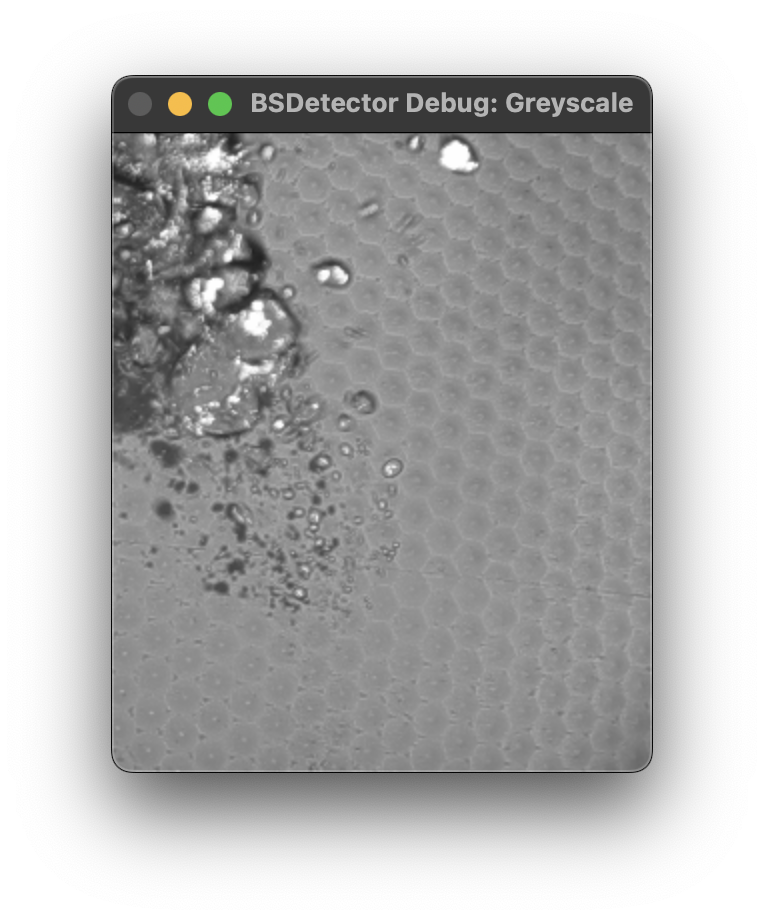
\includegraphics[width=1\linewidth]{assets/sys_gs.png}
            \caption{}
            \label{fig:sys_gs}
        \end{subfigure}
        \hfill
        \begin{subfigure}{0.32\textwidth}
            \centering
            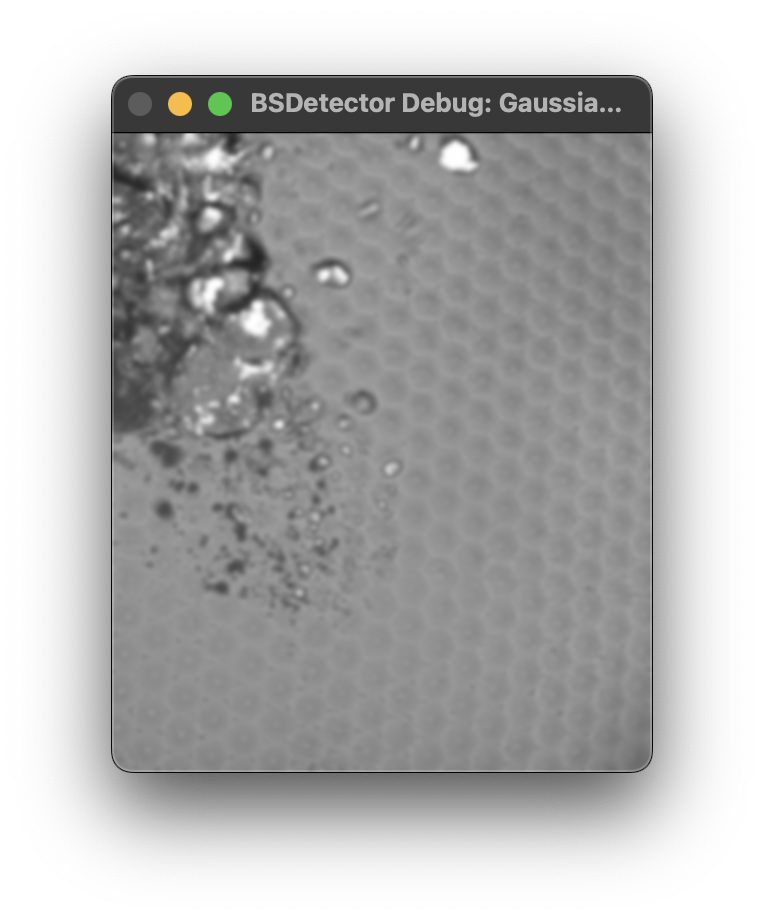
\includegraphics[width=1\linewidth]{assets/sys_gb.png}
            \caption{}
            \label{fig:sys_gb}
        \end{subfigure}
        \hfill
        \begin{subfigure}{0.32\textwidth}
            \centering
            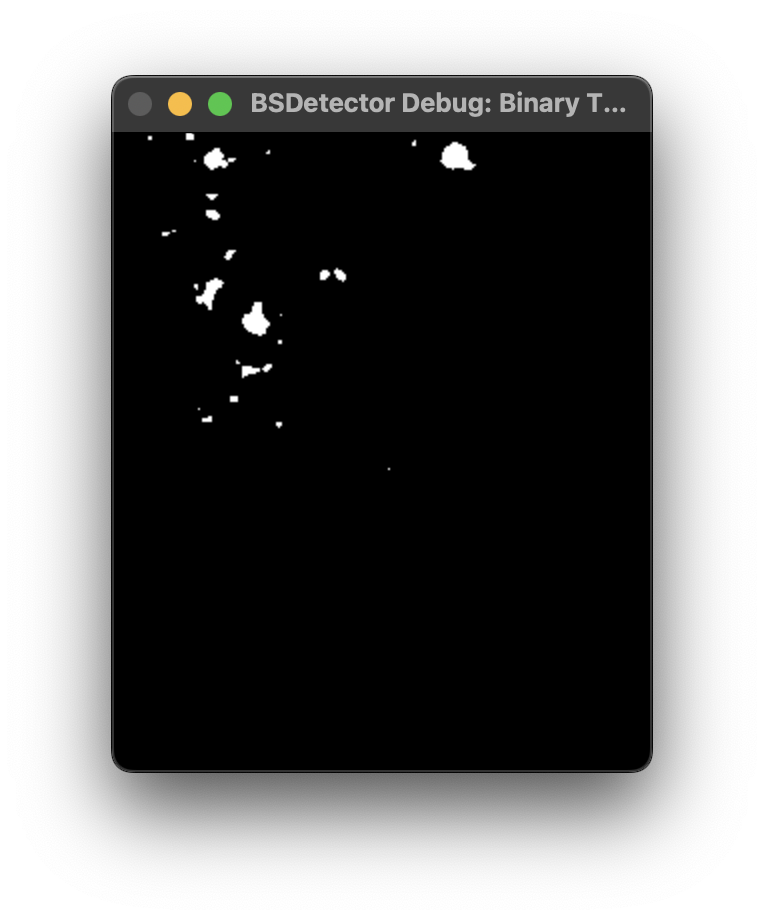
\includegraphics[width=1\linewidth]{assets/sys_thresh.png}
            \caption{}
            \label{fig:sys_thresh}
        \end{subfigure}
        \hfill
        \begin{subfigure}{0.32\textwidth}
            \centering
            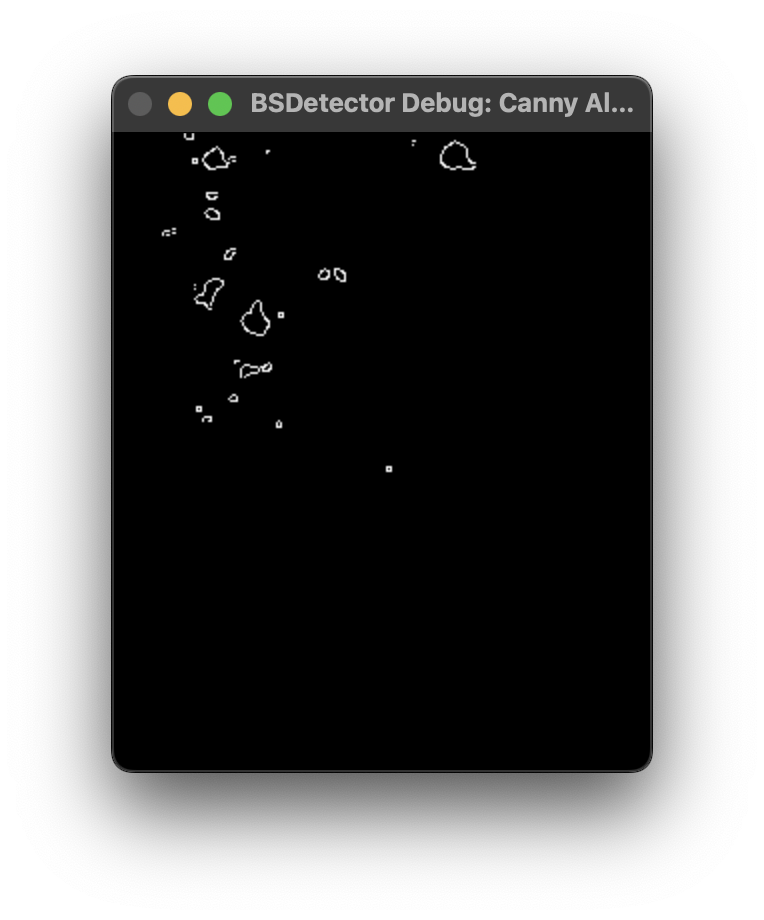
\includegraphics[width=1\linewidth]{assets/sys_canny.png}
            \caption{}
            \label{fig:sys_canny}
        \end{subfigure}
        \hfill
        \begin{subfigure}{0.32\textwidth}
            \centering
            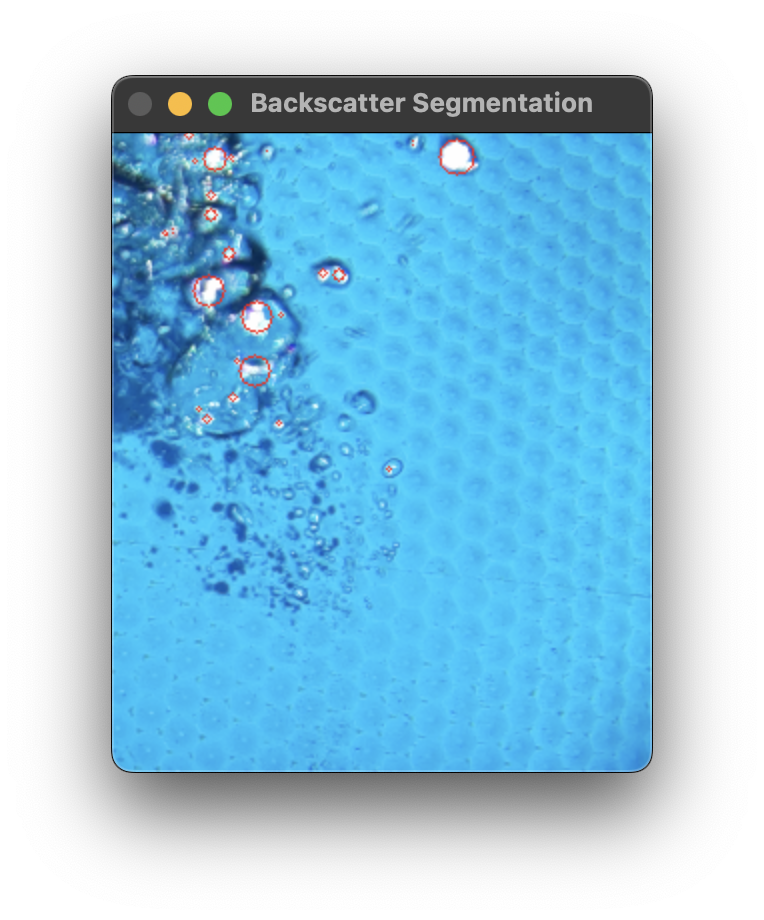
\includegraphics[width=1\linewidth]{assets/sys_segment.png}
            \caption{}
            \label{fig:sys_segment}
        \end{subfigure}
    \end{subfigure}
    \hfill
    \begin{subfigure}{.39\textwidth}
        \centering
        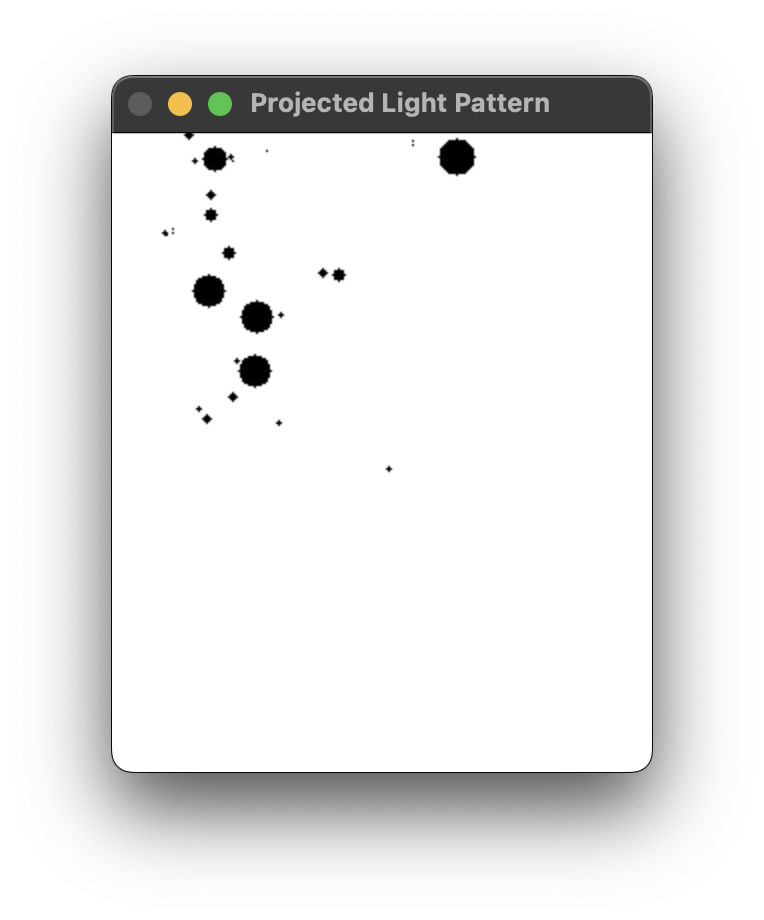
\includegraphics[width=1\linewidth]{assets/sys_project.png}
        \caption{}
        \label{fig:sys_projection}
    \end{subfigure}
    \caption{Screenshots previewing the image processing pipeline stages of the Cancellation System program, in order from left to right: (\ref{sub@fig:sys_input}) the input, (\ref{sub@fig:sys_gs}) greyscale filtering, (\ref{sub@fig:sys_gb}) Gaussian blur, (\ref{sub@fig:sys_thresh}) binary thresholding, (\ref{sub@fig:sys_canny}) the Canny algorithm, (\ref{sub@fig:sys_segment}) segmentation with minimum enclosing circles, finally, (\ref{sub@fig:sys_projection}), the projection.}
    \label{fig:sys_flow_visual}
\end{figure}

\subsection{Performance Evaluation}

Due to time constraints, I couldn't implement logic in the backscatter cancellation system which exports a dataset of detected backscatter particles, which I could've then used to compare with the simulation export, the synthetic ground truth, to quantify the accuracy performance of the system. Therefore, this section entirely focuses on the real-time performance, by analysing the execution time for each image processing pipeline, and the total execution time for each frame with the underwater testing tank footage input to the RPi SBC system with the system software `nice' value set to the lowest value (-20), ensuring the highest process priority, ultimately quantifying the impact of multiprocessing and the PREEMPT-RT kernel patch.

\begin{table}[H]
    \centering
    \begin{tabularx}{\linewidth}{c || X | X | X | X || X | X | X | X}
        \hline
        \multirow[c]{2}{*}{\textbf{Process}} & \multicolumn{4}{c||}{\textbf{Avg. Duration (\textbf{\textmu s})}} & \multicolumn{4}{c}{\textbf{Std. Deviation (\textbf{\textmu s})}}\\
        \cline{2-9}
         & \scriptsize{Std, SP} & \scriptsize{RT, SP} & \scriptsize{Std, MP} & \scriptsize{RT, MP} & \scriptsize{Std, SP} & \scriptsize{RT, SP} & \scriptsize{Std, MP} & \scriptsize{RT, MP} \\
        \hline
        \hline
        Frame Capture & 1,480 & 20,100 & 12,120 & 27,730 & 3199 & 9629 & 14990 & 11600 \\
        \hline
        Greyscale Filter & 193.4 & 2370 & 220.2 & 212.0 & 31.19 & 57.67 & 91.02 & 80.16 \\
        \hline
        Gaussian Blur & 159.2 & 319.2 & 339.5 & 378.8 & 148.2 & 457.4 & 653.0 & 599.0 \\
        \hline
        Binary Threshold & 19.79 & 29.70 & 64.10 & 81.34 & 5.144 & 61.15 & 57.45 & 111.3 \\
        \hline
        Canny Algorithm & 601.9 & 795.3 & 879.20 & 975.3 & 95.46 & 550.3 & 724.4 & 1427 \\
        \hline
        Find Contours & 110.8 & 135.8 & 180.0 & 252.2 & 43.16 & 184.2 & 134.0 & 389.2 \\
        \hline
        Find MECs & 41.88 & 47.14 & 45.60 & 47.05 & 30.84 & 36.67 & 92.65 & 41.89 \\
        \hline
        \hline
        \textbf{Tot. Duration (\textbf{\textmu s})} & 2,607 & 21,620 & 13,850 & 29,670 & 3253 & 9732 & 15140 & 11920 \\
        \hline
    \end{tabularx}
    \caption{Table of real-time metrics for the system using the standard (std.) and real-time (RT) kernel, in single-core mode (SP), and with multiprocessing (MP), all values rounded up to the nearest 4 significant figures.}
    \label{table:sys_std_sp_metrics}
\end{table}

Table \ref{table:sys_std_sp_metrics} transcribes the real-time metrics for the system, across 402 frames of real test footage recorded from the testing tank, listing the execution duration for all the image processing pipeline stages using the standard kernel, real-time kernel, multiprocessing, and in the standard single core mode under the GIL. The data shows a 431\% increase in total latency from the single-core to the multi-core program with the standard kernel, and 37\& increase of that in the real-time kernel, a 729\% increase when moving from the standard to the real-time kernel with single-core, and a 114\% increase when moving from that in the multiprocessing system. The data also contains the standard deviation of the individual processing stage and total system latencies to measure data variability, showing a 199\% increase in fluctuations when moving from the standard to real-time kernel in the single-code environment, and a 21\% decrease of that in the multiprocessing environment.

In contrast to the theory that previous sections cover regarding the reduction of latency with multiprocessing and a real-time OS, the data illustrates the complete opposite. The multiprocessing system employs queues, a form of Inter-Process Communication (IPC), to preserve data whilst processing asynchronously across multiple processes. However, IPCs introduce vast computational overhead due to the requirement of data serialisation and deserialisation when transmitting across processes and during OS context switching. Furthermore, while multiprocessing offers parallelism, it still cannot overcome the synchronous nature of I/O bound processes, as the data quantifies showing a 719\% increase in frame capture durations between the standard single-core and standard multiprocessing systems. The PREEMPT-RT patch, similarly in theory, should've reduced system latency, but most importantly it should've at least resulted in more constant latency measurements. However, the data proves the opposite. The PREEMPT-RT patch increases the frequency of preemption points in the kernel, resulting in more context switches, and when paired with the IPCs, slowing down the system rate and increasing latency.

In summary, the PREEMPT-RT patch greatly alters the kernel behaviour, and due to time constraints, I was unable to successfully profile, research and analyse the effects and pinpoint the exact cause for the latency increase, however it is clear that trying to modify the kernel behaviour from such an abstracted level causes more negative responses, than doing so from a low system level, proving that it is better to leave these tasks to the OS, which is specialised in correctly optimising processes much better than me. To conclude, my single-core RPi SBC system achieves a total processing latency of just \SI{2.6}{\milli\second}, a great improvement from the system in De Charette et al., which takes \SI{4.1}{\milli\second} to process frames on a much more powerful desktop computer, and achieving the \SI{33.33}{\milli\second} (30FPS) target that I had originally set in Section \ref{designsystem}.


\section{Conclusion}
\label{conclusion}
This project set out to design, implement, and evaluate a real-time backscatter cancellation system for underwater imaging, leveraging an RPi SBC for portability and accessibility. The project began by developing the toolsets for the final system, including a backscatter simulation to generate a synthetic ground truth to test and validate the final system, and a lossless recording script to capture underwater footage to test the final system without requiring underwater deployment. These toolsets provided crucial assistance in the final system's development.

The project achieves the objective of precise backscatter particle segmentation by employing an image processing pipeline centred around the Canny edge detection algorithm and a simple minimum enclosing circle segmentation method. The project uncovers mixed results when reducing system latency with a real-time kernel and multiprocessing for increasing system throughput to achieve the latency targets, including the adverse effects of the real-time kernel patch for Linux and Python multiprocessing. However, the single-core system achieves a commendable \SI{2.6}{\milli\second} average frame processing latency, a clear improvement over previous research. Underwater testing of the system, with the lossless recording program, uncovered the drastic parallax and distortion effects due to the submersible housing construction, which resulted in the project's shift from focusing on the development of a final working system, to real-time software optimisation, to balance the short project time duration. Therefore, driving the DLP projector, including functionality to control and establish a fixed system frame rate, was no longer an actionable item. Appendix \ref{gantt} illustrates the evolution of the project schedule using Gantt charts.

In conclusion, this project successfully delivers a functional and efficient backscatter segmentation system, meeting real-time targets. The insights gained from the performance evaluation highlight the intricacies of optimising such systems and suggest that, for specific applications, simpler single-core implementations may offer superior performance compared to more complex multiprocessing or RTOS-enhanced solutions. In addition to completing the objectives for DLP-driven projections and fine-grain framerate controls, the following aspects for future work can drastically improve the system: (a) FPGA implementation for accelerated image processing and DLP projector driving by harnessing the inherently multithreaded architecture, (b) improved submersible housing, mitigating the component offsets with high-precision alignment and a beamsplitter to eliminate parallax by co-location, and finally, (c), a predictive system to track and estimate the future location of backscatter particles to mitigate backscatter movement against system latencies, with options to incorporate machine-learning technologies, using a more realistic backscatter simulation for training data.


%--/Paper--

\newpage
\bibliographystyle{IEEEtranSid}
\bibliography{IEEEabrv,references}

\newpage
\begin{appendices}
    \section{Bubble Backscatter Simulator}
    \label{sim}
    \subsection{Description of Class Fields \& Methods}
\label{sim_tbls}
\begin{table}[H]
    \centering
    \begin{tabularx}{\linewidth}{c | X}
        Name    &   Description\\
        \hline
        \hline
        \texttt{WINDOW\_WIDTH}          &   The maximum width of the simulation window.\\
        \hline
        \texttt{WINDOW\_HEIGHT}         & The maximum height of the simulation window.\\
        \hline
        \texttt{SIMULATION\_FPS}        & The frame rate to simulate.\\
        \hline
        \texttt{MAX\_VELOCITY\_X}       & The maximum possible x-axis velocity for particles.\\
        \hline
        \texttt{MIN\_VELOCITY\_X}   & The minimum possible x-axis velocity for particles.\\
        \hline
        \texttt{MAX\_VELOCITY\_Y}   & The maximum possible y-axis velocity for particles.\\
        \hline
        \texttt{MAX\_VELOCITY\_X}       & The minimum possible y-axis velocity for particles.\\
        \hline
        \texttt{VELOCITY\_CHANGE\_RATE}     & The rate at which the velocity changes.\\
        \hline
        \texttt{MAX\_RADIUS}    & The maximum possible spawn-time particle radius.\\
        \hline
        \texttt{MIN\_RADIUS}    & The minimum possible spawn-time particle radius.\\
        \hline
        \texttt{HEIGHT\_RADIUS\_GROW\_MULTIPLIER}   & The particle radius growth rate as the particle rises.\\
        \hline
        \texttt{BG\_COLOUR}  & The background colour of the simulation window.\\
        \hline
        \texttt{PARTICLE\_COLOUR}  & The particle colour the simulation backscatter.\\
        \hline
        \texttt{MAX\_PARTICLES}  & The maximum possible particles in each frame.\\
        \hline
        \texttt{CONSTANT\_PARTICLE\_GENERATION}  & Option to constantly spawn particles.\\
        \hline
        \texttt{PARTICLE\_RANDOMISE\_VELOCITY\_PROB}  & The probability of particle movement randomisation.\\
        \hline
    \end{tabularx}
    \caption{Simulation parameter constants and their descriptions from the Bubble Backscatter Generator program.}
    \label{table:simbubbleclassparams}
\end{table}

\begin{table}[H]
    \centering
    \begin{tabularx}{\linewidth}{c | X}
        Name    &   Description\\
        \hline
        \hline
        \texttt{id}          &   The unique ID of the particle, generated by \texttt{uuid.uuid4()}.\\
        \hline
        \texttt{x}                       &   The x-axis coordinate position of the particle.\\
        \hline
        \texttt{y}                       &   The y-axis coordinate position of the particle.\\
        \hline
        \texttt{radius}                  &   The radius of the particle.\\
        \hline
        \texttt{velocity\_x}             &   The current x-axis velocity of the particle.\\
        \hline
        \texttt{velocity\_y}             &   The current y-axis velocity of the particle.\\
        \hline
        \texttt{target\_velocity\_x}     &   The target future x-axis velocity of the particle.\\
        \hline
        \texttt{target\_velocity\_y}     &   The target future y-axis velocity of the particle.\\
        \hline
    \end{tabularx}
    \caption{Fields and their descriptions from the Bubble class of the Bubble Backscatter Generator program.}
    \label{table:simbubbleclassfields}
\end{table}

\begin{table}[H]
    \centering
    \begin{tabularx}{\linewidth}{c | X}
        Name    &   Description\\
        \hline
        \hline
        \texttt{\_\_init\_\_()}     &   Initialises a new backscatter \texttt{Bubble} object, generating a unique \texttt{id} with \texttt{uuid.uuid4()}, a random \texttt{x} starting position, \texttt{y} starting position at the bottom of the screen, random \texttt{target\_velocity\_x} and \texttt{target\_velocity\_y} velocities which are set equal to the initial velocities, \texttt{velocity\_x} and \texttt{velocity\_y}.\\
        \hline
        \texttt{randomiseVelocities()} & Generates a random value for \texttt{target\_velocity\_y} and \texttt{target\_velocity\_x}, with the value between \texttt{MIN\_VELOCITY\_Y}, \texttt{MAX\_VELOCITY\_Y}, and \texttt{MIN\_VELOCITY\_X}, \texttt{MAX\_VELOCITY\_X}.\\
        \hline
        \texttt{move()} & Updates the particle's \texttt{x} and \texttt{y} positions based on its \texttt{velocity\_x} and \texttt{velocity\_y} and the simulation time since the last frame. Also updates the particle's velocities, based on the difference between the current velocity and the target velocity, with the \texttt{VELOCITY\_CHANGE\_RATE} multiplier.\\
        \hline
        \texttt{draw()} & Draws the particle based on its \texttt{x} and \texttt{y} positions, and \texttt{radius}, with the colour from the \texttt{PARTICLE\_COLOUR} constant, using the Pygame library's \texttt{pygame.draw.circle()} function.\\
        \hline
    \end{tabularx}
    \caption{Methods and their descriptions from the Bubble class of the Bubble Backscatter Generator program.}
    \label{table:simbubbleclassfuncs}
\end{table}

\subsection{Python Code}
\label{sim_code}
\lstinputlisting[language=Python, caption={The Python code for the Bubble Backscatter Simulator, commit version: \texttt{34b9a82} from \href{https://github.com/Sidharth-Shanmugam-MEng-Project-2023-24/bubble-backscatter-simulator/blob/main/app.py}{https://github.com/Sidharth-Shanmugam-MEng-Project-2023-24/bubble-backscatter-simulator/blob/main/app.py}}]{code/00_bubble-backscatter-simulator/app.py}


    \section{Lossless Video Recorder}
    \label{pirec}
    \subsection{Description of Class Fields \& Methods}
\label{rec_tbls}
\begin{table}[H]
    \centering
    \begin{tabularx}{\linewidth}{c | X}
        Name    &   Description\\
        \hline
        \hline
        \texttt{REC\_FPS}          &   The recording frame rate.\\
        \hline
        \texttt{REC\_WIDTH}         & The horizontal resolution of recording.\\
        \hline
        \texttt{REC\_HEIGHT}         & The vertical resolution of recording.\\
        \hline
        \texttt{FB\_WIDTH}         &  The horizontal resolution of the Framebuffer.\\
        \hline
        \texttt{FB\_HEIGHT}         & The vertical resolution of the Framebuffer.\\
        \hline
        \texttt{FB\_DEPTH}          & The bit depth of the Framebuffer.\\
        \hline
    \end{tabularx}
    \caption{Software configuration constants and their descriptions from the Lossless Raspberry Pi Camera Recorder program.}
    \label{table:recparams}
\end{table}

\subsubsection{The `ProjectorManager' Module}

\begin{table}[H]
    \centering
    \begin{tabularx}{\linewidth}{c | X}
        Name    &   Description\\
        \hline
        \hline
        \texttt{width} & The horizontal resolution of the Framebuffer device, same as \texttt{FB\_WIDTH}.\\
        \hline
        \texttt{height} & The vertical resolution of the Framebuffer device, same as \texttt{FB\_HEIGHT}.\\
        \hline
        \texttt{height} & The Framebuffer bit depth, same as \texttt{FB\_DEPTH}.\\
        \hline
        \texttt{status} & Stores \texttt{True} if the projector light is `on', \texttt{False} if `off'.\\
        \hline
    \end{tabularx}
    \caption{Fields and their descriptions from the Projector class of the `ProjectorManager' module from the Lossless Raspberry Pi Camera Recorder program.}
    \label{table:projectormanagerclassfields}
\end{table}

\begin{table}[H]
    \centering
    \begin{tabularx}{\linewidth}{c | X}
        Name    &   Description\\
        \hline
        \hline
        \texttt{\_\_init\_\_()}     &   Initialises a new \texttt{Projector} object, populating the Framebuffer fields for \texttt{FB\_WIDTH}, \texttt{FB\_HEIGHT}, and \texttt{FB\_DEPTH}. Initialising the bitmaps for light `on' and `off', and setting the light status to `off'.\\
        \hline
        \texttt{getStatus()}     &   A simple `getter' function for the \texttt{status} class field.\\
        \hline
        \texttt{on()}     &   Writes the `on' bitmap to the Framebuffer memory location, thus turning on the projector light source.\\
        \hline
        \texttt{off()}     &   Writes the `off' bitmap to the Framebuffer memory location, thus turning off the projector light source.\\
        \hline
        \texttt{toggle()}     &   Writes the `on' bitmap to the Framebuffer memory location if the \texttt{status} stores `off', and vice-versa, thus toggling on the projector light source.\\
        \hline
    \end{tabularx}
    \caption{Methods and their descriptions from the Projector class of the `ProjectorManager' module from the Lossless Raspberry Pi Camera Recorder program.}
    \label{table:projectormanagerclassfuncs}
\end{table}

\subsubsection{The `CameraManager' Module}

\begin{table}[H]
    \centering
    \begin{tabularx}{\linewidth}{c | X}
        Name    &   Description\\
        \hline
        \hline
        \texttt{picam2} & Stores the initialised \texttt{Picamera2} instance.\\
        \hline
        \texttt{recording} & Stores \texttt{True} if the recording is in progress, otherwise stores \texttt{True}.\\
        \hline
        \texttt{recording\_filename} & Stores the filename which the recorded file will be saved as.\\
        \hline
        \texttt{recording\_start\_ts} & Stores the timestamp of when the recording was started.\\
        \hline
        \texttt{recording\_end\_ts} & Stores the timestamp of when the recording was stopped.\\
        \hline
    \end{tabularx}
    \caption{Fields and their descriptions from the Camera class of the `CameraManager' module from the Lossless Raspberry Pi Camera Recorder program.}
    \label{table:cameramanagerclassfields}
\end{table}

\begin{table}[H]
    \centering
    \begin{tabularx}{\linewidth}{c | X}
        Name    &   Description\\
        \hline
        \hline
        \texttt{\_\_init\_\_()}     &   Initalises and configures the \texttt{Picamera2} instance by setting the recording resolution from \texttt{REC\_WIDTH} and \texttt{REC\_HEIGHT}, the frame rate from \texttt{REC\_RATE}, capture stream as the `main' output stream, and an ISP output format as `BGR888', and finally starts the RPi Camera module.\\
        \hline
        \texttt{getStatus()}     &   A simple `getter' function for the \texttt{recording} class field.\\
        \hline
        \texttt{captureFrame()}     &   Retrieves and returns the camera's sensor output array.\\
        \hline
        \texttt{startRecording()}     &   Sets the \texttt{recording} class field to \texttt{True}, then initialises a memory buffer, logging the timestamp for \texttt{recording\_start\_ts} before finally initialising the `Null' encoder and starting the recording.\\
        \hline
        \texttt{stopRecording()}     &   Sets the \texttt{recording} class field to \texttt{False}, then stops the `Picamera2' recording, before applying the lossless FFV1 encoding to the footage bitstream, then finally writing to a file and closing the memory buffer.\\
        \hline
        \texttt{toggleRecording()}     &   Starts a recording if not already recording, and vice-versa, thus toggling the Pi Camera recording.\\
        \hline
        \texttt{shutdown()}     &   Stops recording if there is one in progress before finally sending a graceful shutdown signal to the `Picamera2' module to stop and disconnect the Pi Camera.\\
        \hline
    \end{tabularx}
    \caption{Methods and their descriptions from the Camera class of the `CameraManager' module from the Lossless Raspberry Pi Camera Recorder program.}
    \label{table:cameramanagerclassfuncs}
\end{table}

\subsubsection{The `PreviewManager' Module}

\begin{table}[H]
    \centering
    \begin{tabularx}{\linewidth}{c | X}
        Name    &   Description\\
        \hline
        \hline
        \texttt{\_\_init\_\_()}     &   Initalises a new OpenCV-based GUI window.\\
        \hline
        \texttt{getKeypress()}     &   Retrieves a keypress using the OpenCV GUI functions.\\
        \hline
        \texttt{shutdown()}     &   Destroys the OpenCV GUI window.\\
        \hline
        \texttt{showFrame()}     &   Renders the image frame on the GUI window and overlays the status variable text using OpenCV.\\
        \hline
    \end{tabularx}
    \caption{Methods and their descriptions from the Preview class of the `PreviewManager' module from the Lossless Raspberry Pi Camera Recorder program.}
    \label{table:previewmanagerclassfuncs}
\end{table}


\subsection{Python Code}
\label{rec_code}
\subsubsection{Entry Point: `app.py'}

\lstinputlisting[language=Python, caption={The Python code for the `app.py' entry point to the Lossless Raspberry Pi Camera Recorder, commit version: \texttt{30efb5a} from \href{https://github.com/Sidharth-Shanmugam-MEng-Project-2023-24/picam-video-recorder/blob/main/app.py}{https://github.com/Sidharth-Shanmugam-MEng-Project-2023-24/picam-video-recorder/blob/main/app.py}}]{code/01_picam-recorder/app.py}


\subsubsection{ProjectorManger: `ProjectorManager.py'}

\lstinputlisting[language=Python, caption={The Python code for `ProjectorManager.py' in the Lossless Raspberry Pi Camera Recorder, commit version: \texttt{30efb5a} from \href{https://github.com/Sidharth-Shanmugam-MEng-Project-2023-24/picam-video-recorder/blob/main/ProjectorManager.py}{https://github.com/Sidharth-Shanmugam-MEng-Project-2023-24/picam-video-recorder/blob/main/ProjectorManager.py}}]{code/01_picam-recorder/ProjectorManager.py}


\subsubsection{CameraManager: `CameraManager.py'}

\lstinputlisting[language=Python, caption={The Python code for `CameraManager.py' in the Lossless Raspberry Pi Camera Recorder, commit version: \texttt{30efb5a} from \href{https://github.com/Sidharth-Shanmugam-MEng-Project-2023-24/picam-video-recorder/blob/main/CameraManager.py}{https://github.com/Sidharth-Shanmugam-MEng-Project-2023-24/picam-video-recorder/blob/main/CameraManager.py}}]{code/01_picam-recorder/CameraManager.py}


\subsubsection{PreviewManager: `PreviewManager.py'}

\lstinputlisting[language=Python, caption={The Python code for `PreviewManager.py' in the Lossless Raspberry Pi Camera Recorder, commit version: \texttt{30efb5a} from \href{https://github.com/Sidharth-Shanmugam-MEng-Project-2023-24/picam-video-recorder/blob/main/PreviewManager.py}{https://github.com/Sidharth-Shanmugam-MEng-Project-2023-24/picam-video-recorder/blob/main/PreviewManager.py}}]{code/01_picam-recorder/PreviewManager.py}



    \section{Standard Backscatter Cancellation System}
    \label{sys}
    \subsection{Description of Class Fields \& Methods}
\label{sys_tbls}
\begin{table}[H]
    \centering
    \begin{tabularx}{\linewidth}{c | X}
        Name    &   Description\\
        \hline
        \hline
        \texttt{VIDEO\_CAPTURE\_SOURCE} & Set with directory path to input a list of individual frames, file path to input a video file, or integer `0' to use the RPi Camera input.\\
        \hline
        \texttt{VIDEO\_CAPTURE\_WIDTH} & The horizontal resolution of recording.\\
        \hline
        \texttt{VIDEO\_CAPTURE\_HEIGHT} & The vertical resolution of recording.\\
        \hline
        \texttt{VIDEO\_CAPTURE\_CROP\_HEIGHT} &  The vertical resolution to crop for the region of interest.\\
        \hline
        \texttt{VIDEO\_CAPTURE\_CROP\_WIDTH} &  The horizontal resolution to crop for the region of interest.\\
        \hline
        \texttt{BS\_MANAGER\_DEBUG\_WINDOWS} & Whether to render debug windows showing the post-processed frame after intermediate processing stages.\\
        \hline
    \end{tabularx}
    \caption{Software configuration constants and their descriptions from the Backscatter Cancellation program.}
    \label{table:sysparams}
\end{table}

\subsection{Python Code}
\label{sys_code}
\subsubsection{Entry Point: `app.py'}

\lstinputlisting[language=Python, caption={The Python code for the `app.py' entry point to the Backscatter Cancellation System program, commit version: \texttt{46b962a} from \href{https://github.com/Sidharth-Shanmugam-MEng-Project-2023-24/backscatter-cancellation-system/blob/main/app.py}{https://github.com/Sidharth-Shanmugam-MEng-Project-2023-24/backscatter-cancellation-system/blob/main/app.py}}]{code/02_system/app.py}

\subsubsection{CaptureManager: `CaptureManager.py'}

\lstinputlisting[language=Python, caption={The Python code for `CaptureManager.py' in the Backscatter Cancellation System program, commit version: \texttt{1bf8131} from \href{https://github.com/Sidharth-Shanmugam-MEng-Project-2023-24/backscatter-cancellation-system/blob/main/CaptureManager.py}{https://github.com/Sidharth-Shanmugam-MEng-Project-2023-24/backscatter-cancellation-system/blob/main/CaptureManager.py}}]{code/02_system/CaptureManager.py}

\subsubsection{BSManager: `BSManager.py'}

\lstinputlisting[language=Python, caption={The Python code for `BSManager.py' in the Backscatter Cancellation System program, commit version: \texttt{46b962a} from \href{https://github.com/Sidharth-Shanmugam-MEng-Project-2023-24/backscatter-cancellation-system/blob/main/BSManager.py}{https://github.com/Sidharth-Shanmugam-MEng-Project-2023-24/backscatter-cancellation-system/blob/main/BSManager.py}}]{code/02_system/BSManager.py}

\subsubsection{TimeManager: `TimeManager.py'}

\lstinputlisting[language=Python, caption={The Python code for `TimeManager.py' in the Backscatter Cancellation System program, commit version: \texttt{2367e84} from \href{https://github.com/Sidharth-Shanmugam-MEng-Project-2023-24/backscatter-cancellation-system/blob/main/TimeManager.py}{https://github.com/Sidharth-Shanmugam-MEng-Project-2023-24/backscatter-cancellation-system/blob/main/TimeManager.py}}]{code/02_system/TimeManager.py}

\subsubsection{WindowManager: `WindowManager.py'}

\lstinputlisting[language=Python, caption={The Python code for `WindowManager.py' in the Backscatter Cancellation System program, commit version: \texttt{407ac01} from \href{https://github.com/Sidharth-Shanmugam-MEng-Project-2023-24/backscatter-cancellation-system/blob/main/WindowManager.py}{https://github.com/Sidharth-Shanmugam-MEng-Project-2023-24/backscatter-cancellation-system/blob/main/WindowManager.py}}]{code/02_system/WindowManager.py}


    \section{Multiprocessing Backscatter Cancellation System}
    \label{mpsys}
    \subsection{Python Code}
\label{sysmp_code}
\subsubsection{Entry Point: `app2.py'}

\lstinputlisting[language=Python, caption={The Python code for the `app2.py' entry point to the Multiprocessing Backscatter Cancellation System program, commit version: \texttt{326e3b5} from \href{https://github.com/Sidharth-Shanmugam-MEng-Project-2023-24/backscatter-cancellation-system/blob/multiprocessing/app2.py}{https://github.com/Sidharth-Shanmugam-MEng-Project-2023-24/backscatter-cancellation-system/blob/multiprocessing/app2.py}}]{code/03_system-mp/app2.py}

\subsubsection{CaptureManager: `CaptureManager.py'}

\lstinputlisting[language=Python, caption={The Python code for `CaptureManager.py' in the Multiprocessing Backscatter Cancellation System program, commit version: \texttt{1e69d8b} from \href{https://github.com/Sidharth-Shanmugam-MEng-Project-2023-24/backscatter-cancellation-system/blob/multiprocessing/CaptureManager.py}{https://github.com/Sidharth-Shanmugam-MEng-Project-2023-24/backscatter-cancellation-system/blob/multiprocessing/CaptureManager.py}}]{code/02_system/CaptureManager.py}

\subsubsection{TimeManager: `TimeManager.py'}
Use the same \texttt{TimeManager.py} from the Standard Backscatter Cancellation System.

\subsubsection{WindowManager: `WindowManager.py'}
Use the same \texttt{WindowManager.py} from the Standard Backscatter Cancellation System.


    \section{Project Progress Gantt Charts}
    \label{gantt}
    \subsection{08-03-2024}

\begin{figure}[H]
    \centering
    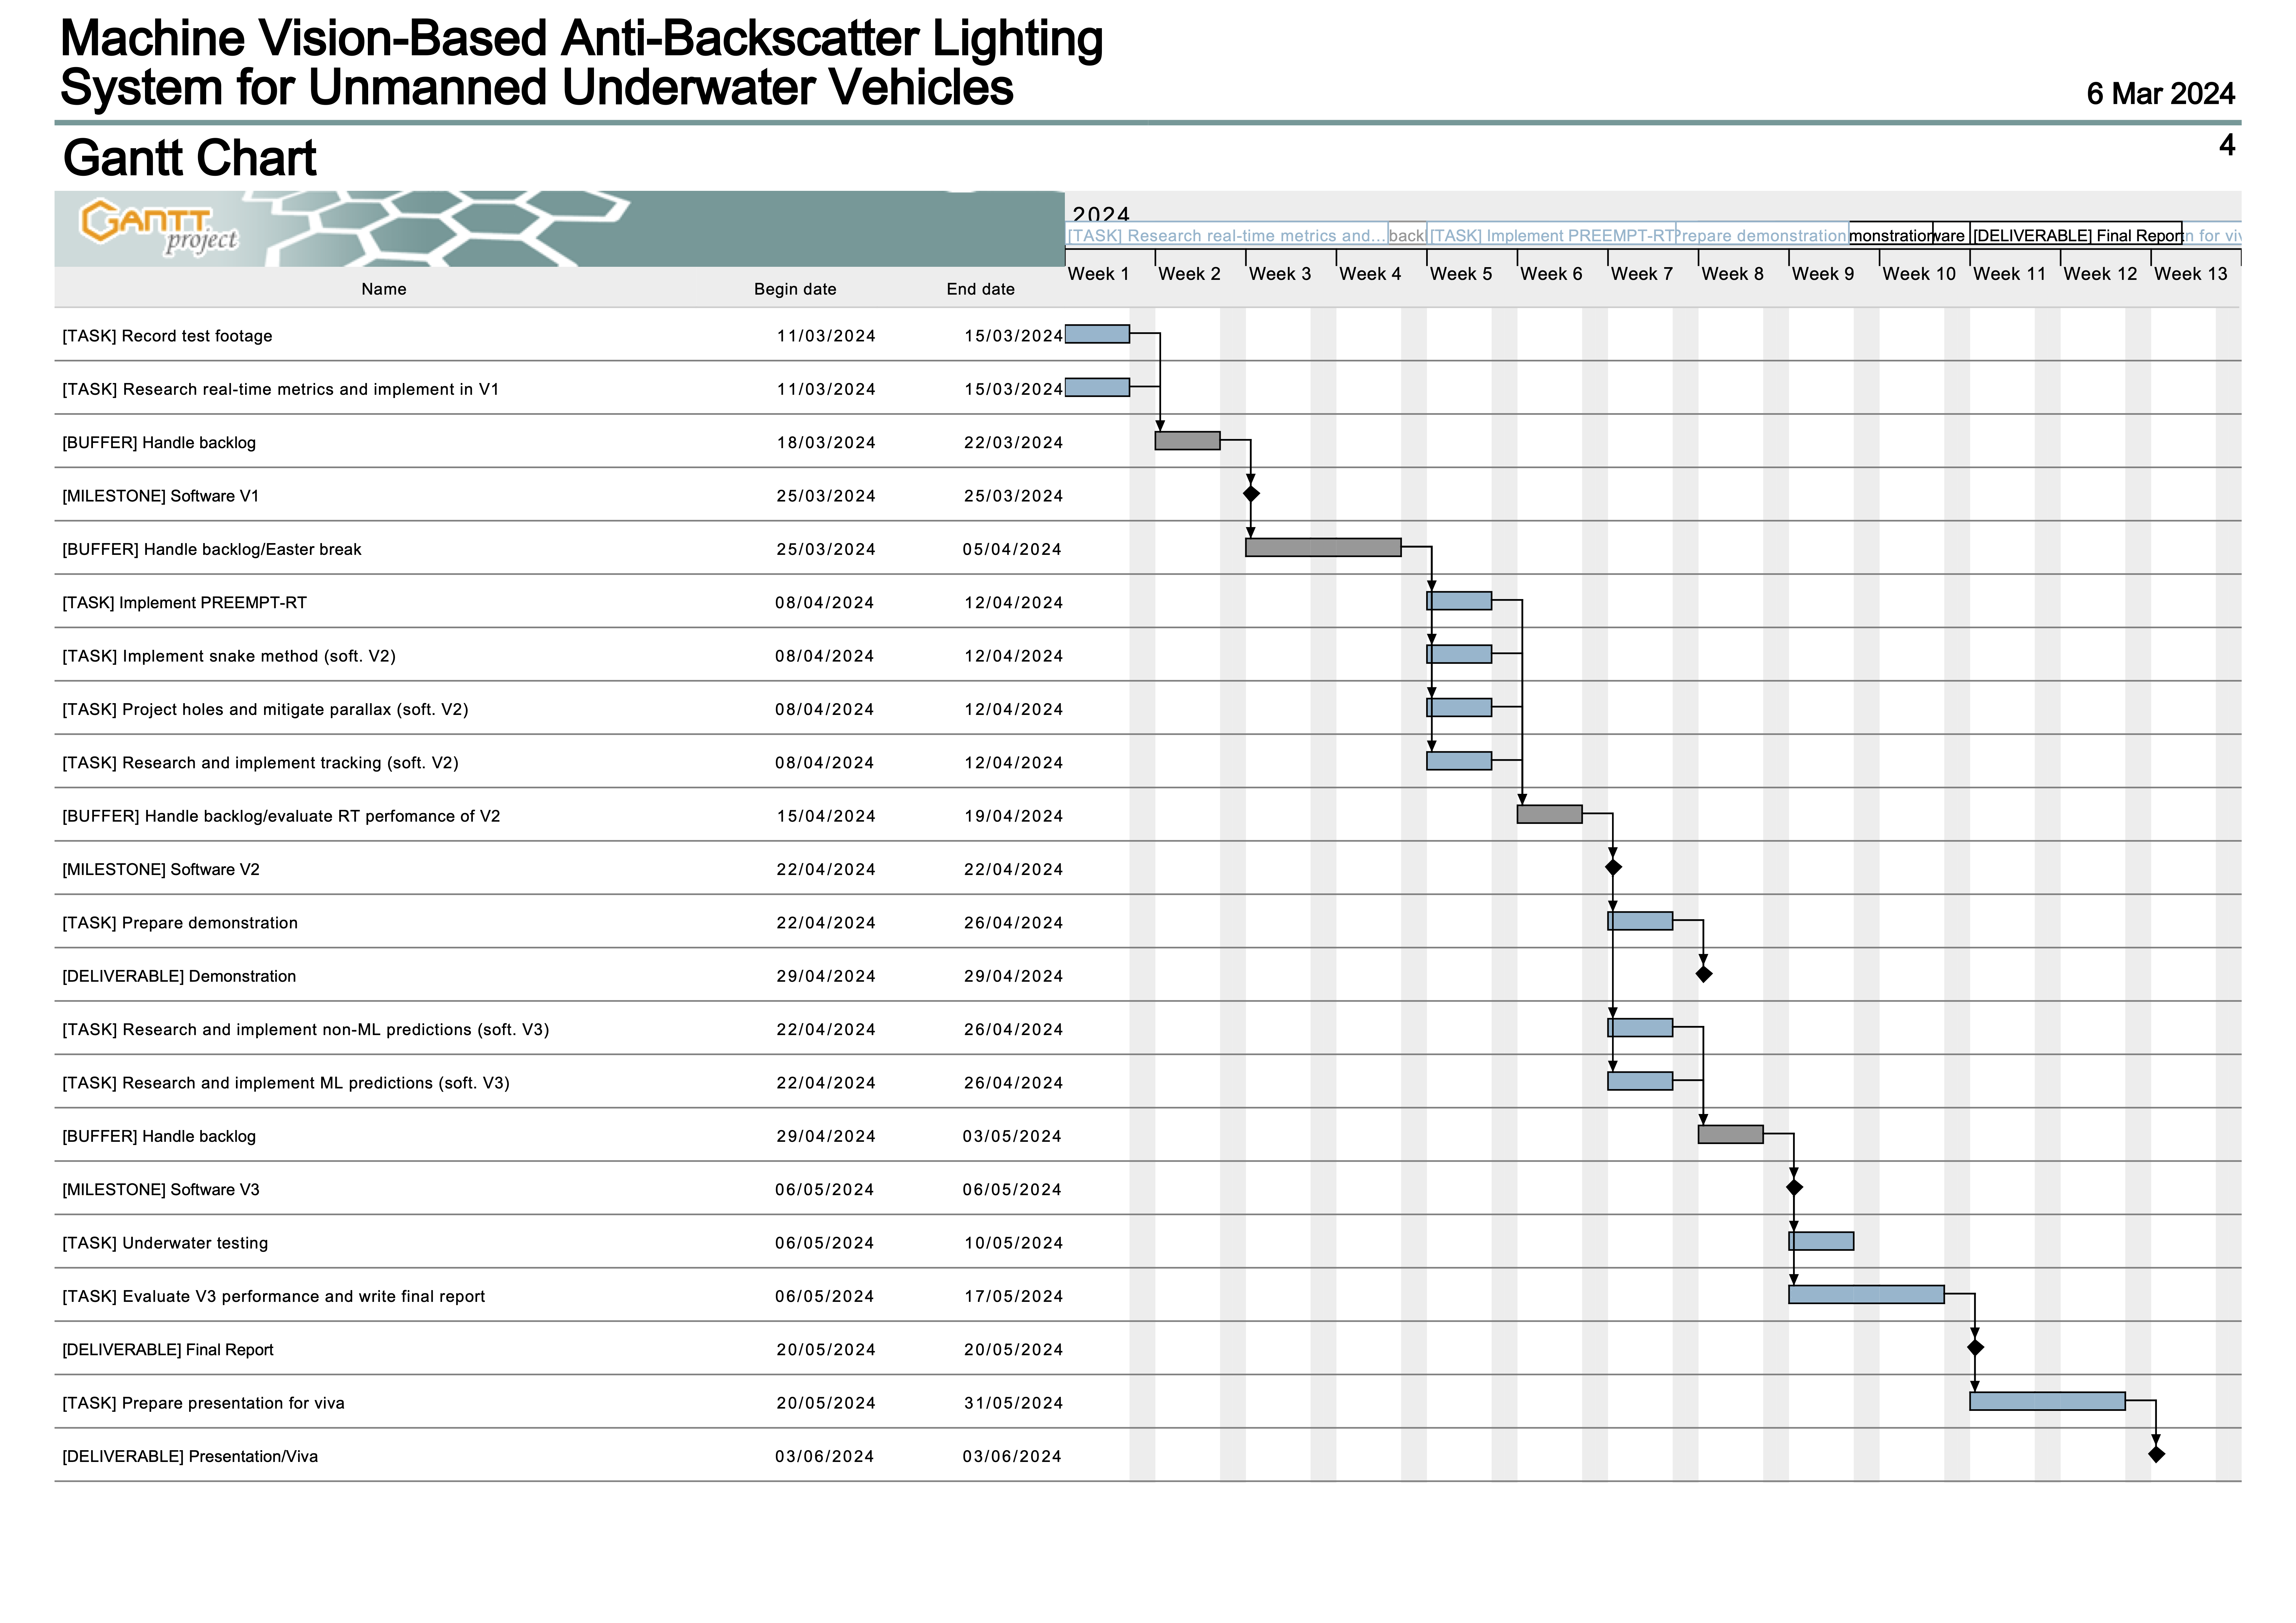
\includegraphics[width=1\textwidth]{assets/gantt1.png}
    \caption{Gantt chart schedule as of the 8\textsuperscript{th} of March, 2024.}
    \label{fig:gantt1}
\end{figure}

\subsection{15-03-2024}

\begin{figure}[H]
    \centering
    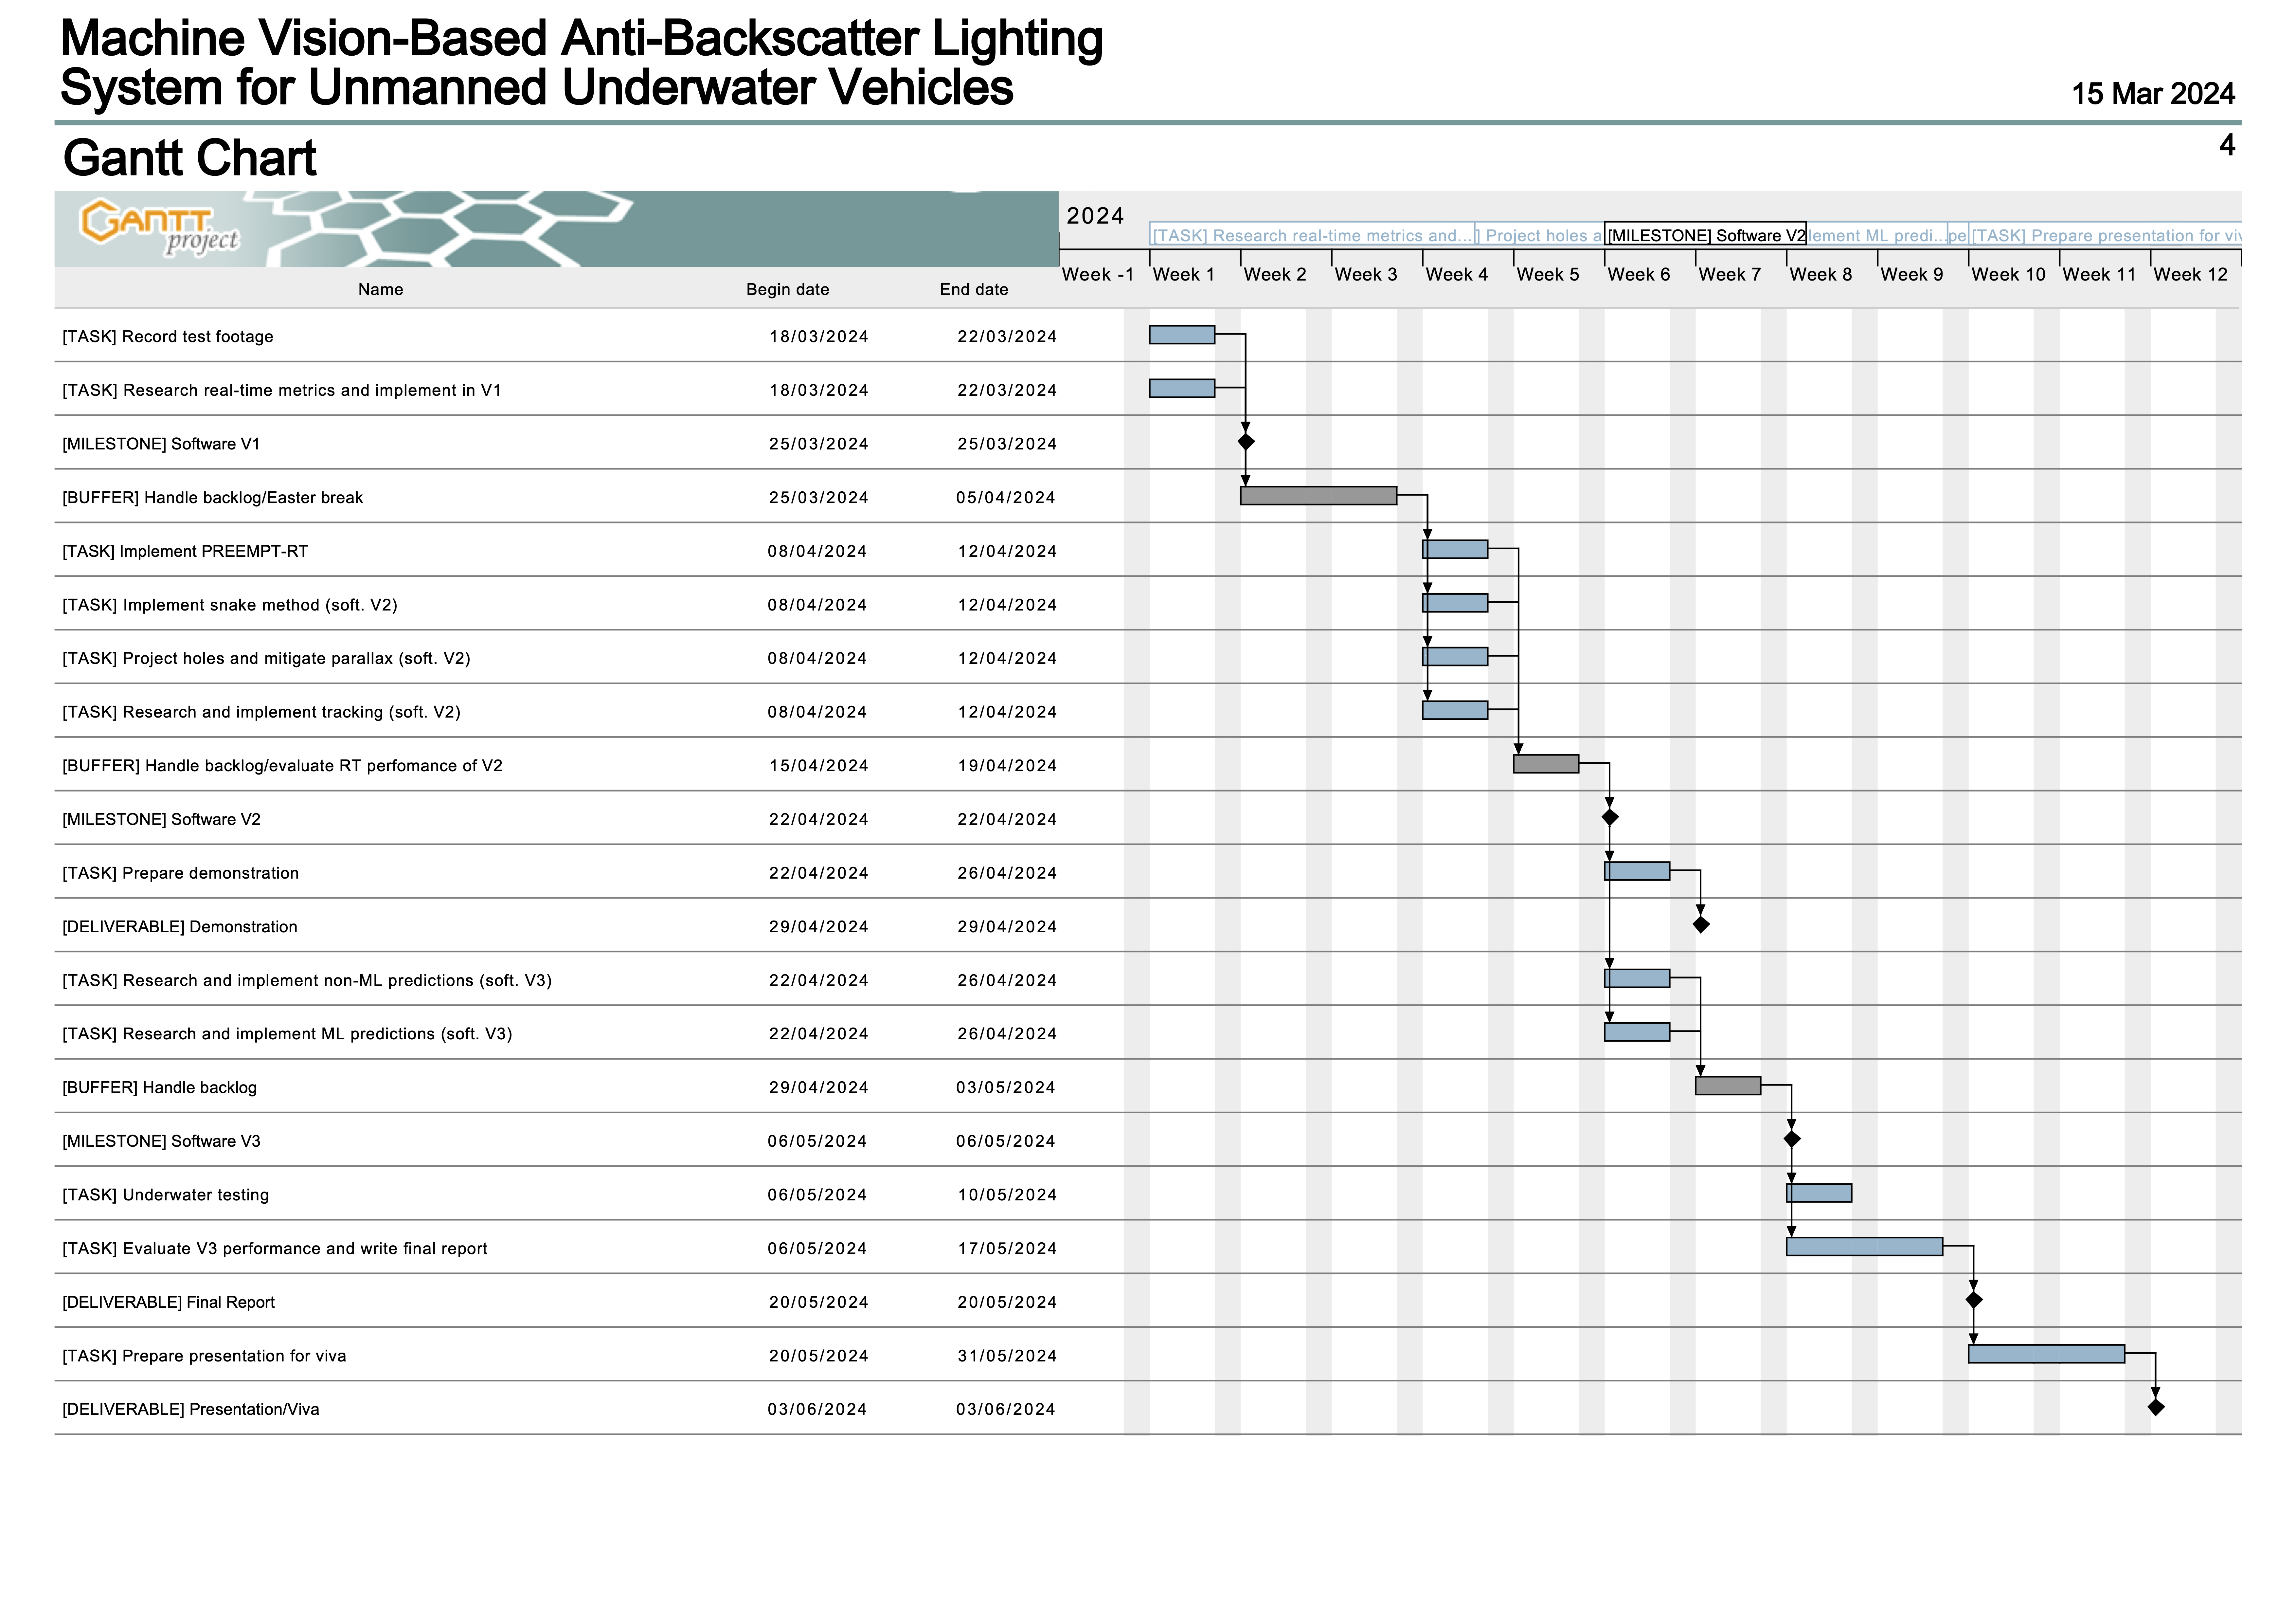
\includegraphics[width=1\textwidth]{assets/gantt2.png}
    \caption{Gantt chart schedule as of the 15\textsuperscript{th} of March, 2024.}
    \label{fig:gantt2}
\end{figure}

\subsection{12-04-2024}

\begin{figure}[H]
    \centering
    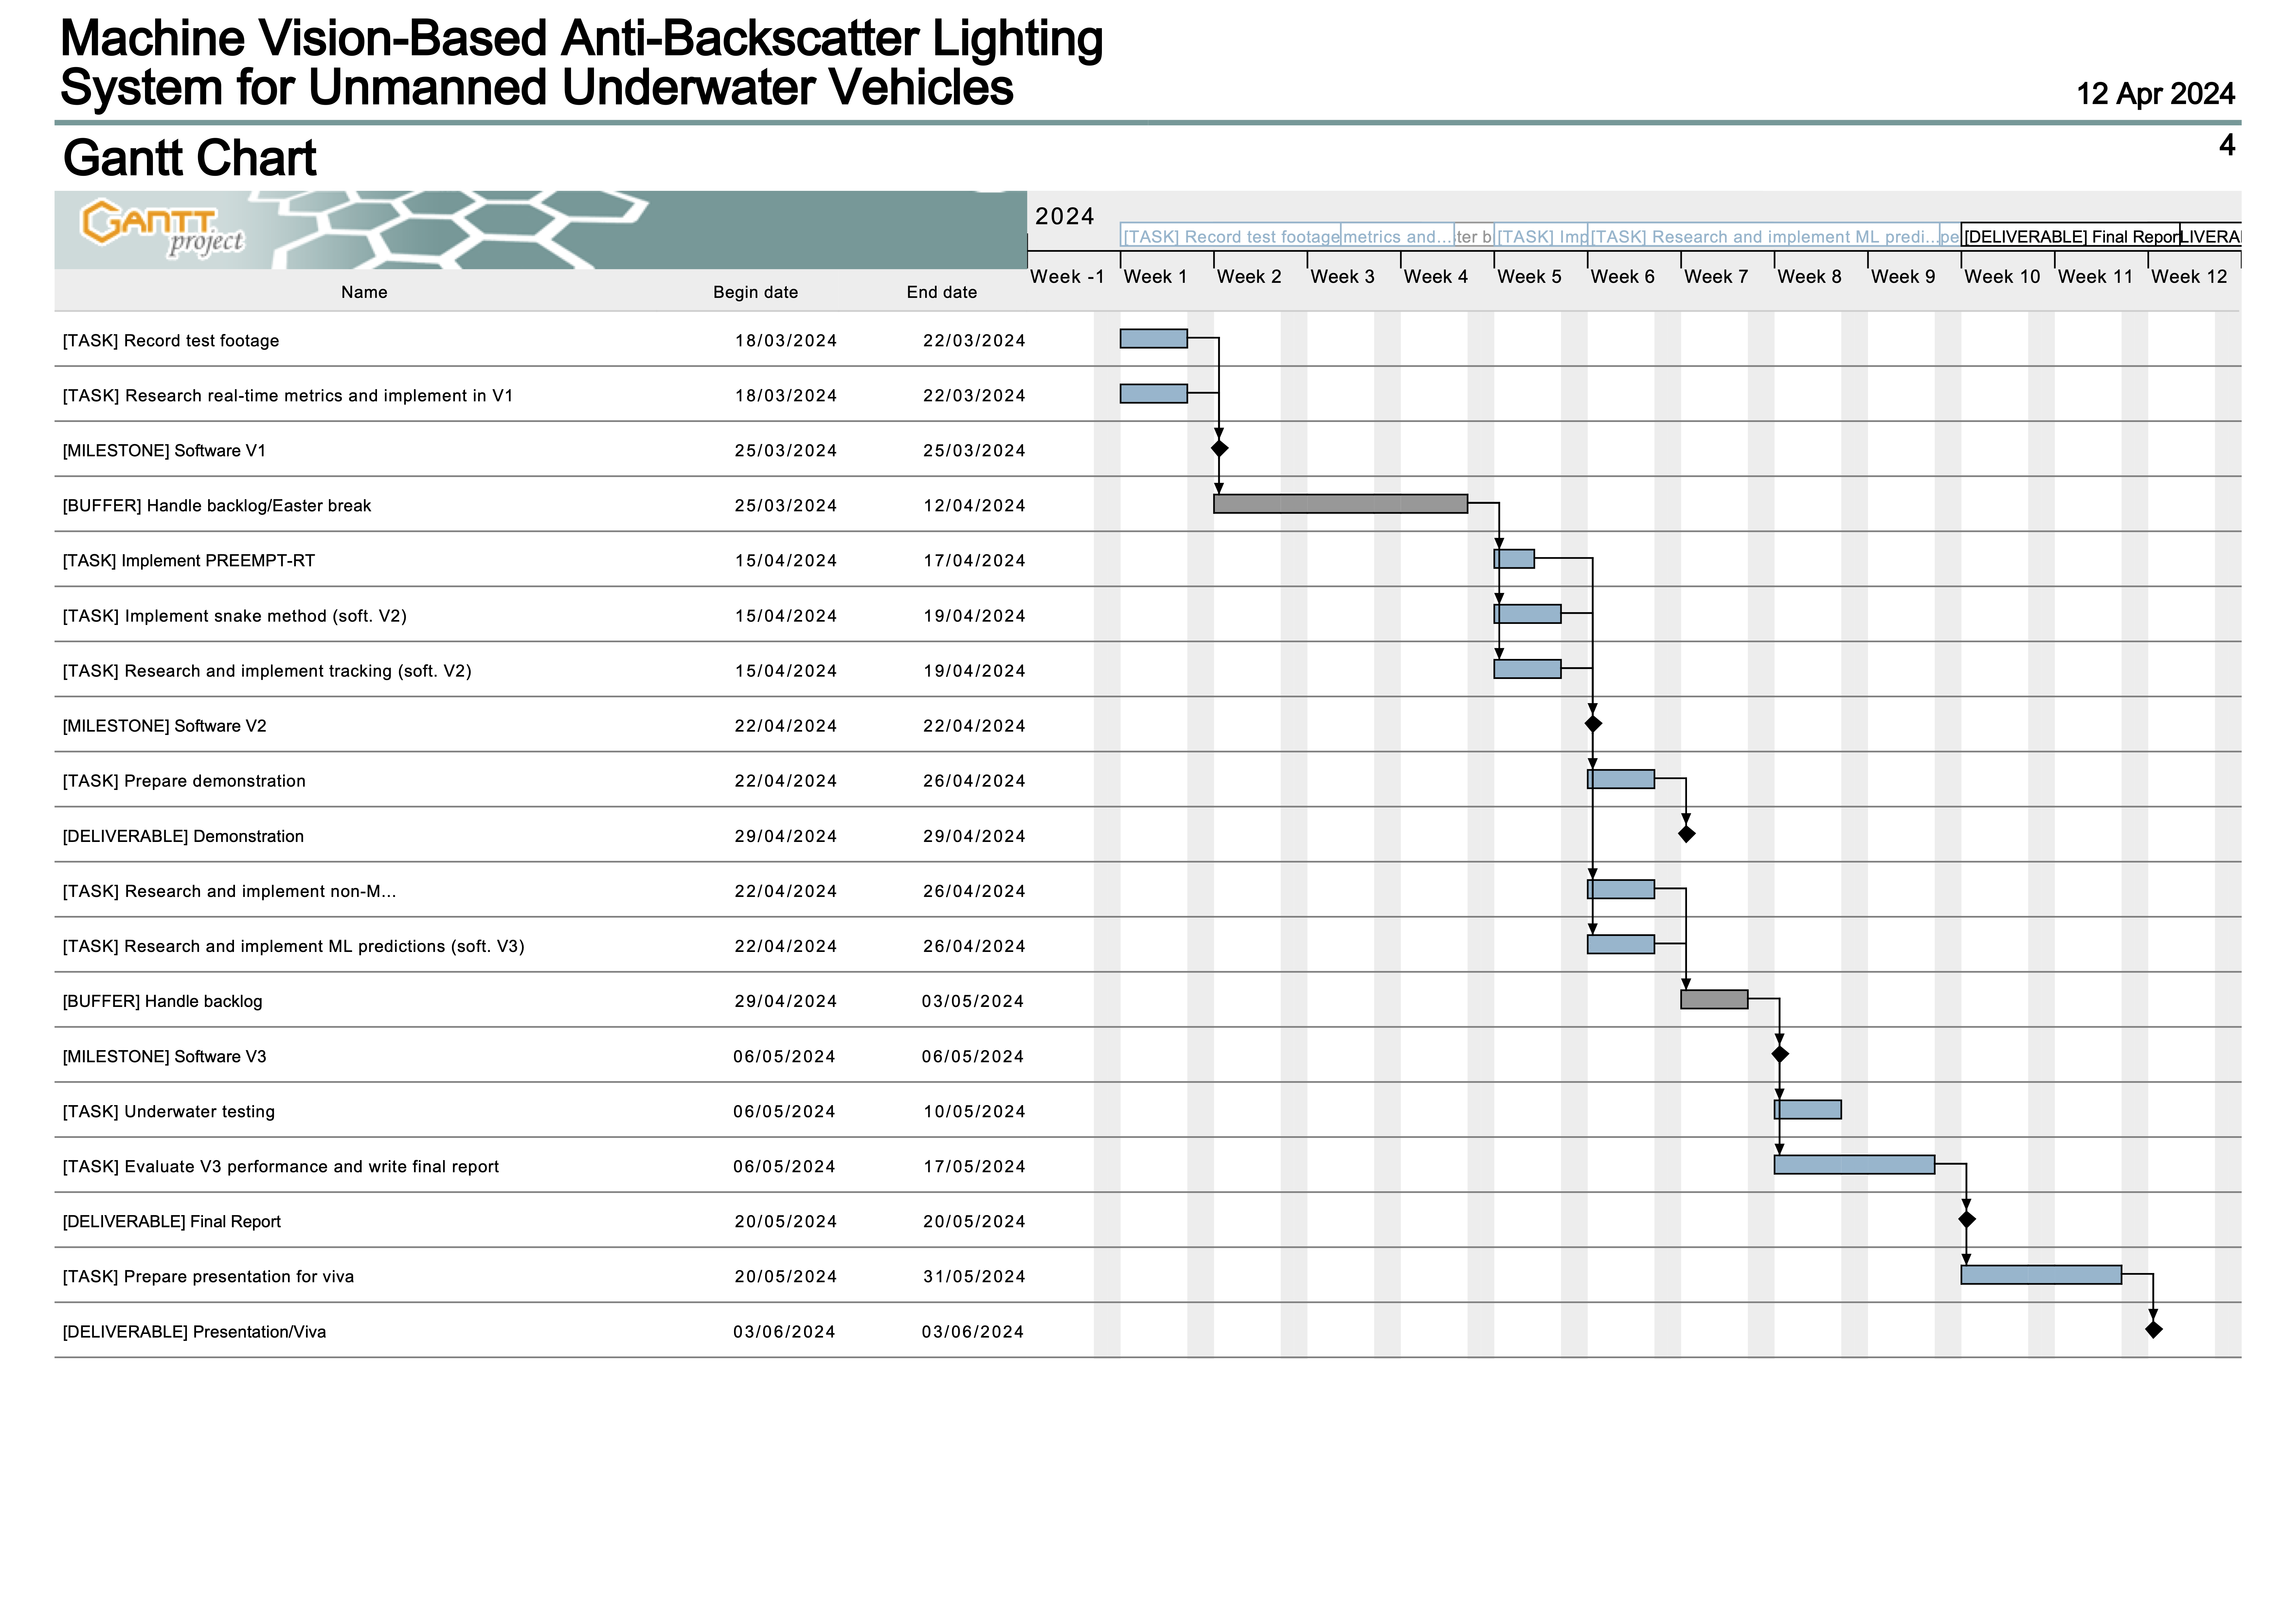
\includegraphics[width=1\textwidth]{assets/gantt3.png}
    \caption{Gantt chart schedule as of the 12\textsuperscript{th} of April, 2024.}
    \label{fig:gantt3}
\end{figure}

\subsection{03-05-2024}

\begin{figure}[H]
    \centering
    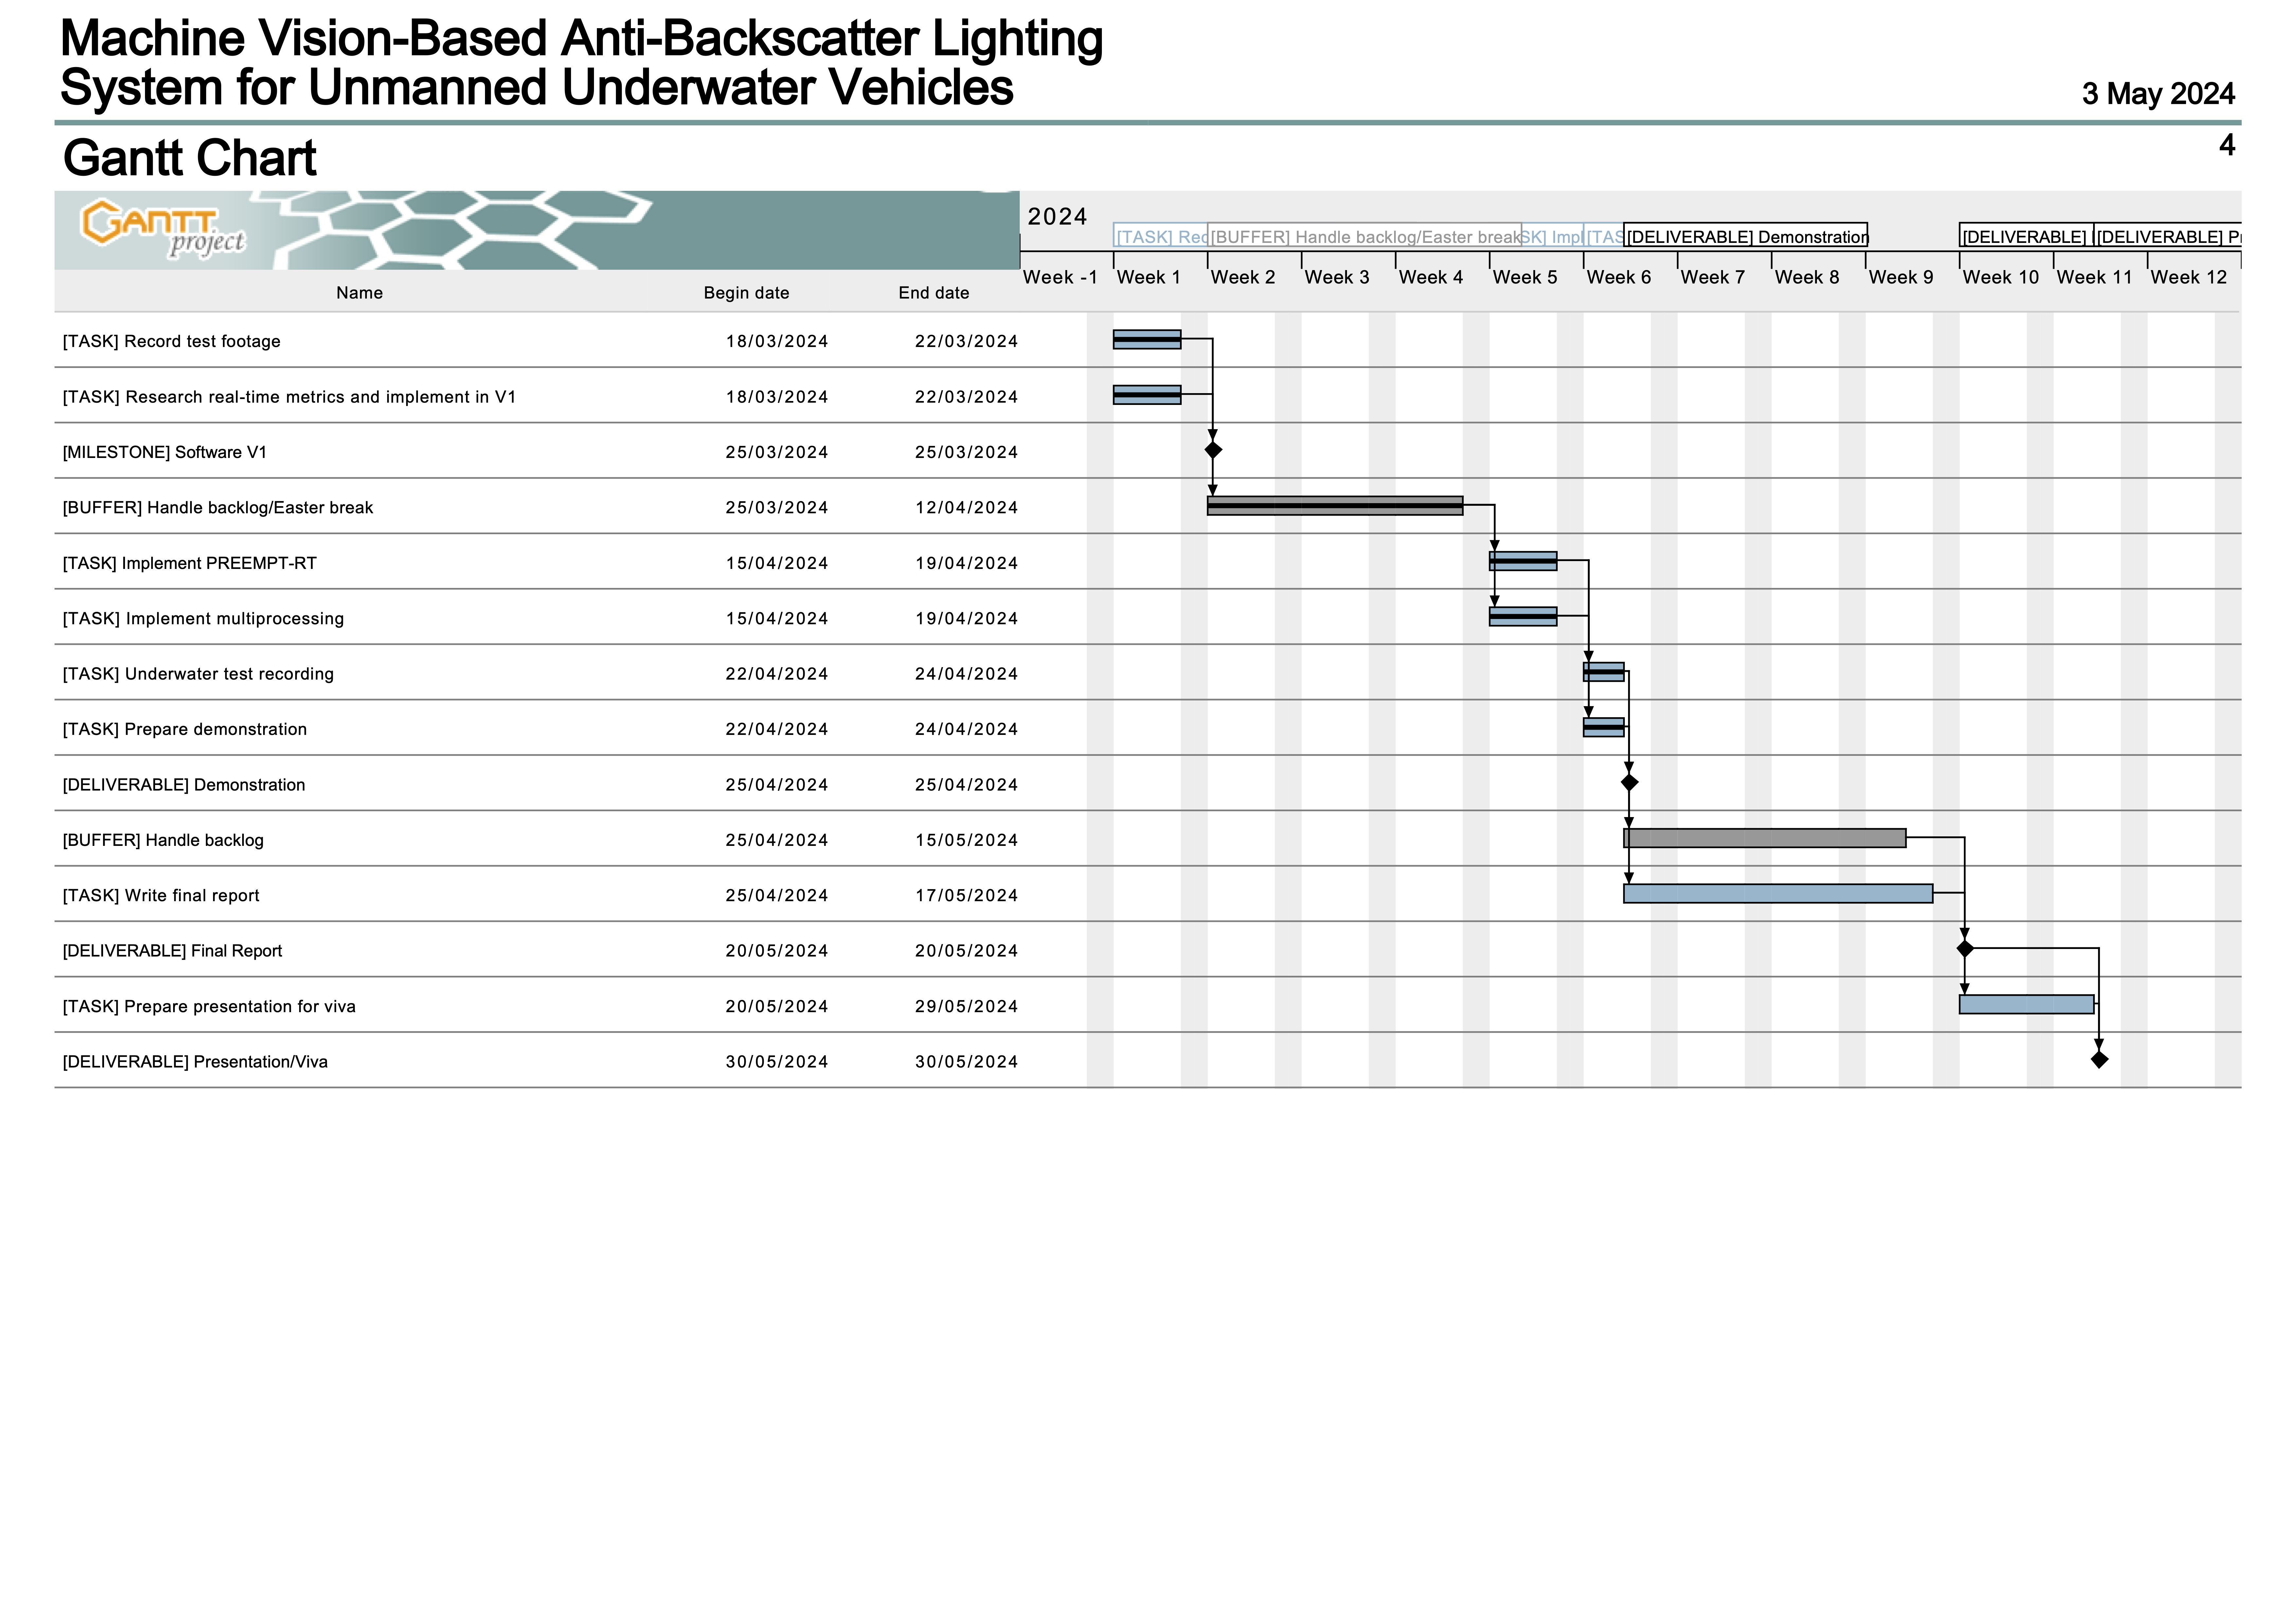
\includegraphics[width=1\textwidth]{assets/gantt4.png}
    \caption{Gantt chart schedule as of the 3\textsuperscript{rd} of May, 2024.}
    \label{fig:gantt4}
\end{figure}
\end{appendices}

\end{document}
